\documentclass[11pt,a4paper]{iopthsis}
\usepackage{alltt,chicago,float}
% \usepackage{chapterbib}
\usepackage{epsfig,graphicx}

%%% -*-TeX-*-
%%% ====================================================================
%%%  @TeX-file{
%%%     author          = "Tom Rokicki",
%%%     version         = "2.7.4",
%%%     date            = "14 February 2011",
%%%     time            = "15:44:06 MST",
%%%     filename        = "epsf.tex",
%%%     address         = "Tom Rokicki
%%%                        Box 2081
%%%                        Stanford, CA 94309
%%%                        USA",
%%%     telephone       = "+1 415 855 9989",
%%%     checksum        = "29223 653 3100 27123",
%%%     email           = "rokicki@cs.stanford.edu (Internet)",
%%%     codetable       = "ISO/ASCII",
%%%     copyright       = "This file is freely redistributable and
%%%                        placed into the public domain by Tomas
%%%                        Rokicki.",
%%%     keywords        = "PostScript, TeX",
%%%     license         = "public domain",
%%%     supported       = "yes",
%%%     abstract        = "This file contains macros to support the
%%%                        inclusion of Encapsulated PostScript files
%%%                        in TeX documents.",
%%%     docstring       = "This file contains TeX macros to include an
%%%                        Encapsulated PostScript graphic.  It works
%%%                        by finding the bounding box comment,
%%%                        calculating the correct scale values, and
%%%                        inserting a vbox of the appropriate size at
%%%                        the current position in the TeX document.
%%%
%%%                        To use, simply use
%%%
%%%                        \input epsf % somewhere early on in your TeX file
%%%
%%%                        % then where you want to insert a vbox for a figure:
%%%                        \epsfbox{filename.ps}
%%%
%%%                        Alternatively, you can supply your own
%%%                        bounding box by
%%%
%%%                        \epsfbox[0 0 30 50]{filename.ps}
%%%
%%%                        This will not read in the file, and will
%%%                        instead use the bounding box you specify.
%%%
%%%                        The effect will be to typeset the figure as
%%%                        a TeX box, at the point of your \epsfbox
%%%                        command. By default, the graphic will have
%%%                        its `natural' width (namely the width of
%%%                        its bounding box, as described in
%%%                        filename.ps). The TeX box will have depth
%%%                        zero.
%%%
%%%                        You can enlarge or reduce the figure by
%%%                        using
%%%
%%%                          \epsfxsize = <dimen> \epsfbox{filename.ps}
%%%                        or
%%%                          \epsfysize = <dimen> \epsfbox{filename.ps}
%%%
%%%                        instead. Then the width of the TeX box will
%%%                        be \epsfxsize and its height will be scaled
%%%                        proportionately (or the height will be
%%%                        \epsfysize and its width will be scaled
%%%                        proportionately).
%%%
%%%                        The width (and height) is restored to zero
%%%                        after each use, so \epsfxsize or \epsfysize
%%%                        must be specified before EACH use of
%%%                        \epsfbox.
%%%
%%%                        A more general facility for sizing is
%%%                        available by defining the \epsfsize macro.
%%%                        Normally you can redefine this macro to do
%%%                        almost anything.  The first parameter is
%%%                        the natural x size of the PostScript
%%%                        graphic, the second parameter is the
%%%                        natural y size of the PostScript graphic.
%%%                        It must return the xsize to use, or 0 if
%%%                        natural scaling is to be used.  Common uses
%%%                        include:
%%%
%%%                           \epsfxsize  % just leave the old value alone
%%%                           0pt         % use the natural sizes
%%%                           #1          % use the natural sizes
%%%                           \hsize      % scale to full width
%%%                           0.5#1       % scale to 50% of natural size
%%%                           \ifnum #1 > \hsize \hsize \else #1\fi
%%%                                       % smaller of natural, hsize
%%%
%%%                        If you want TeX to report the size of the
%%%                        figure (as a message on your terminal when
%%%                        it processes each figure), use
%%%                        `\epsfverbosetrue'.
%%%
%%%                        If you only want to get the bounding box
%%%                        extents, without producing any output boxes
%%%                        or \special{}, then use \epsfgetbb{filename}.
%%%                        The bounding box corner coordinates are saved
%%%                        in the macros \epsfllx, \epsflly, \epsfurx,
%%%                        and \epsfury in PostScript units of big
%%%                        points.
%%%
%%%                        Revision history:
%%%
%%%                        ---------------------------------------------
%%%                        epsf.tex macro file:
%%%                        Originally written by Tomas Rokicki of
%%%                        Radical Eye Software, 29 Mar 1989.
%%%
%%%                        ---------------------------------------------
%%%                        Revised by Don Knuth, 3 Jan 1990.
%%%
%%%                        ---------------------------------------------
%%%                        Revised by Tomas Rokicki, 18 Jul 1990.
%%%                        Accept bounding boxes with no space after
%%%                        the colon.
%%%
%%%                        ---------------------------------------------
%%%                        Revised by Nelson H. F. Beebe
%%%                        <beebe@math.utah.edu>, 03 Dec 1991 [2.0].
%%%                        Add version number and date typeout.
%%%
%%%                        Use \immediate\write16 instead of \message
%%%                        to ensure output on new line.
%%%
%%%                        Handle nested EPS files.
%%%
%%%                        Handle %%BoundingBox: (atend) lines.
%%%
%%%                        Do not quit when blank lines are found.
%%%
%%%                        Add a few percents to remove generation of
%%%                        spurious blank space.
%%%
%%%                        Move \special output to
%%%                        \epsfspecial{filename} so that other macro
%%%                        packages can input this one, then change
%%%                        the definition of \epsfspecial to match
%%%                        another DVI driver.
%%%
%%%                        Move size computation to \epsfsetsize which
%%%                        can be called by the user; the verbose
%%%                        output of the bounding box and scaled width
%%%                        and height happens here.
%%%
%%%                        ---------------------------------------------
%%%                        Revised by Nelson H. F. Beebe
%%%                        <beebe@math.utah.edu>, 05 May 1992 [2.1].
%%%                        Wrap \leavevmode\hbox{} around \vbox{} with
%%%                        the \special so that \epsffile{} can be
%%%                        used inside \begin{center}...\end{center}
%%%
%%%                        ---------------------------------------------
%%%                        Revised by Nelson H. F. Beebe
%%%                        <beebe@math.utah.edu>, 09 Dec 1992 [2.2].
%%%                        Introduce \epsfshow{true,false} and
%%%                        \epsfframe{true,false} macros; the latter
%%%                        suppresses the insertion of the PostScript,
%%%                        and instead just creates an empty box,
%%%                        which may be handy for rapid prototyping.
%%%
%%%                        ---------------------------------------------
%%%                        Revised by Nelson H. F. Beebe
%%%                        <beebe@math.utah.edu>, 14 Dec 1992 [2.3].
%%%                        Add \epsfshowfilename{true,false}.  When
%%%                        true, and \epsfshowfalse is specified, the
%%%                        PostScript file name will be displayed
%%%                        centered in the figure box.
%%%
%%%                        ---------------------------------------------
%%%                        Revised by Nelson H. F. Beebe
%%%                        <beebe@math.utah.edu>, 20 June 1993 [2.4].
%%%                        Remove non-zero debug setting of \epsfframemargin,
%%%                        and change margin handling to preserve EPS image
%%%                        size and aspect ratio, so that the actual
%%%                        box is \epsfxsize+\epsfframemargin wide by
%%%                        \epsfysize+\epsfframemargin high.
%%%                        Reduce output of \epsfshowfilenametrue to
%%%                        just the bare file name.
%%%
%%%                        ---------------------------------------------
%%%                        Revised by Nelson H. F. Beebe
%%%                        <beebe@math.utah.edu>, 13 July 1993 [2.5].
%%%                        Add \epsfframethickness for control of
%%%                        \epsfframe frame lines.
%%%
%%%                        ---------------------------------------------
%%%                        Revised by Nelson H. F. Beebe
%%%                        <beebe@math.utah.edu>, 02 July 1996 [2.6]
%%%                        Add missing initialization \epsfatendfalse;
%%%                        the lack of this resulted in the wrong
%%%                        BoundingBox being picked up, mea culpa, sigh...
%%%
%%%                        ---------------------------------------------
%%%                        Revised by Nelson H. F. Beebe
%%%                        <beebe@math.utah.edu>, 25 October 1996 [2.7]
%%%                        Update to match changes in from dvips 5-600
%%%                        distribution: new user-accessible macros:
%%%                        \epsfclipon, \epsfclipoff, \epsfdrafton,
%%%                        \epsfdraftoff, change \empty to \epsfempty.
%%%
%%%                        ---------------------------------------------
%%%                        Revised by Nelson H. F. Beebe
%%%                        <beebe@math.utah.edu>, 18 May 2002 [2.7.1]
%%%                        Add write statements to echo input file
%%%                        names.  Prior to that change, an error in
%%%                        such a file could be quite hard to track
%%%                        down: a long list of TeX page numbers could
%%%                        suddenly be followed by ``TeX buffer
%%%                        capacity'' exceeded, without any indication
%%%                        of the file that was responsible.
%%%
%%%                        ---------------------------------------------
%%%                        Revised by Nelson H. F. Beebe
%%%                        <beebe@math.utah.edu>, 16 May 2003 [2.7.2]
%%%                        Supply two critical percent characters that
%%%                        were mistakenly omitted in version 2.7.1,
%%%                        and resulted in a small amount of spurious
%%%                        horizontal space.
%%%
%%%                        ---------------------------------------------
%%%                        Revised by Nelson H. F. Beebe
%%%                        <beebe@math.utah.edu>, 14 Feb 2011 [2.7.3]
%%%                        Add previously-missing \space in rwi
%%%                        assignments (bug reported 14-Feb-2011 by
%%%                        Stefan Rueger <s.rueger@open.ac.uk>).
%%%
%%%                        ---------------------------------------------
%%%                        Revised by Nelson H. F. Beebe
%%%                        <beebe@math.utah.edu>, Karl Berry
%%%                        <karl@freefriends.org>, and Robin Fairbairns
%%%                        <Robin.Fairbairns@cl.cam.ac.uk>,
%%%                        23 July 2005 [2.7.3]
%%%                        Add critical \hbox{} wrapper in \epsfsetgraph
%%%                        so that \epsfbox{} does not conflict with
%%%                        LaTeX center environment when \epsfbox{} is
%%%                        surrounded by other horizonal objects.
%%%                        Improve macro readability by adding legal,
%%%                        but invisible-in-typeset-output, spaces.
%%%                        Ensure that verbose status reports come
%%%                        inside (filename ...) list.
%%%
%%%                        ---------------------------------------------
%%%                        The checksum field above contains a CRC-16
%%%                        checksum as the first value, followed by
%%%                        the equivalent of the standard UNIX wc
%%%                        (word count) utility output of lines,
%%%                        words, and characters.  This is produced by
%%%                        Robert Solovay's checksum utility.",
%%%  }
%%% ====================================================================

%\immediate \write16 {This is `epsf.tex' v2.0 <02 Dec 1991>}%
%\immediate \write16 {This is `epsf.tex' v2.1 <05 May 1992>}%
%\immediate \write16 {This is `epsf.tex' v2.2 <09 Dec 1992>}%
%\immediate \write16 {This is `epsf.tex' v2.3 <14 Dec 1992>}%
%\immediate \write16 {This is `epsf.tex' v2.4 <20 June 1993>}%
%\immediate \write16 {This is `epsf.tex' v2.5 <13 July 1993>}%
%\immediate \write16 {This is `epsf.tex' v2.6 <02 July 1996>}%
%\immediate \write16 {This is `epsf.tex' v2.7 <25 October 1996>}%
%\immediate \write16 {This is `epsf.tex' v2.7.1 <18 May 2002>}%
%\immediate \write16 {This is `epsf.tex' v2.7.2 <16 May 2003>}%
%\immediate \write16 {This is `epsf.tex' v2.7.3 <23 July 2005>}%
\immediate \write16 {This is `epsf.tex' v2.7.4 <14 February 2011>}%
%
\newread \epsffilein    % file to \read
\newif \ifepsfatend     % need to scan to LAST %%BoundingBox comment?
\newif \ifepsfbbfound   % success?
\newif \ifepsfdraft     % use draft mode?
\newif \ifepsffileok    % continue looking for the bounding box?
\newif \ifepsfframe     % frame the bounding box?
\newif \ifepsfshow      % show PostScript file, or just bounding box?
\epsfshowtrue          % default is to display PostScript file
\newif \ifepsfshowfilename % show the file name if \epsfshowfalse specified?
\newif \ifepsfverbose   % report what you're making?
\newdimen \epsfframemargin % margin between box and frame
\newdimen \epsfframethickness % thickness of frame rules
\newdimen \epsfrsize    % vertical size before scaling
\newdimen \epsftmp      % register for arithmetic manipulation
\newdimen \epsftsize    % horizontal size before scaling
\newdimen \epsfxsize    % horizontal size after scaling
\newdimen \epsfysize    % vertical size after scaling
\newdimen \pspoints     % conversion factor
%
\pspoints = 1bp        % Adobe points are `big'
\epsfxsize = 0pt       % default value, means `use natural size'
\epsfysize = 0pt       % ditto
\epsfframemargin = 0pt % default value: frame box flush around picture
\epsfframethickness = 0.4pt % TeX's default rule thickness
%
\def \epsfbox #1{%
    \global \def \epsfllx {72}%
    \global \def \epsflly {72}%
    \global \def \epsfurx {540}%
    \global \def \epsfury {720}%
    \def \lbracket {[}%
    \def \testit {#1}%
    \ifx \testit \lbracket
        \let \next = \epsfgetlitbb
    \else
        \let \next = \epsfnormal
    \fi
    \next{#1}%
}%
%
% We use \epsfgetlitbb if the user specified an explicit bounding box,
% and \epsfnormal otherwise.  Because \epsfgetbb can be called
% separately to retrieve the bounding box, we move the verbose
% printing the bounding box extents and size on the terminal to
% \epsfstatus.  Therefore, when the user provided the bounding box,
% \epsfgetbb will not be called, so we must call \epsfsetsize and
% \epsfstatus ourselves.
%
\def \epsfgetlitbb #1#2 #3 #4 #5]#6{%
   \epsfgrab #2 #3 #4 #5 .\\%
   \epsfsetsize
   \epsfstatus{#6}%
   \epsfsetgraph{#6}%
}%
%
\def \epsfnormal #1{%
    \epsfgetbb{#1}%
    \epsfsetgraph{#1}%
}%
%
\def \epsfgetbb #1{%
%
%   The first thing we need to do is to open the
%   PostScript file, if possible.
%
    \openin\epsffilein=#1
    \immediate \write16 {(#1}%
    \ifeof \epsffilein
        \errmessage{Could not open file #1, ignoring it}%
    \else                       %process the file
        {%                      %start a group to contain catcode changes
            % Make all special characters, except space, to be of type
            % `other' so we process the file in almost verbatim mode
            % (TeXbook, p. 344).
            \chardef \other = 12%
            \def \do ##1{\catcode`##1=\other}%
            \dospecials
            \catcode `\ = 10%
            \epsffileoktrue        %true while we are looping
            \epsfatendfalse        %[02-Jul-1996]: add forgotten initialization
            \loop                  %reading lines from the EPS file
                \read \epsffilein to \epsffileline
                \ifeof \epsffilein %then no more input
                \epsffileokfalse   %so set completion flag
            \else                  %otherwise process one line
                \expandafter \epsfaux \epsffileline :. \\%
            \fi
            \ifepsffileok
            \repeat
            \ifepsfbbfound
            \else
                \ifepsfverbose
                    \immediate \write16 {No BoundingBox comment found in %
                                         file #1; using defaults}%
                \fi
            \fi
        }%                      %end catcode changes
        \closein\epsffilein
    \fi                         %end of file processing
    \epsfsetsize                %compute size parameters
    \epsfstatus{#1}%
    \immediate \write16 {)}%
}%
%
% Clipping control:
\def \epsfclipon  {\def \epsfclipstring { clip}}%
\def \epsfclipoff {\def \epsfclipstring {\ifepsfdraft \space clip\fi}}%
\epsfclipoff % default for dvips is OFF
%
% The special that is emitted by \epsfsetgraph comes from this macro.
% It is defined separately to allow easy customization by other
% packages that first \input epsf.tex, then redefine \epsfspecial.
% This macro is invoked in the lower-left corner of a box of the
% width and height determined from the arguments to \epsffile, or
% from the %%BoundingBox in the EPS file itself.
%
% This version is for dvips:
\def \epsfspecial #1{%
     \epsftmp=10\epsfxsize
     \divide \epsftmp by \pspoints
     \ifnum \epsfrsize = 0%
       \relax
       \special{PSfile=\ifepsfdraft psdraft.ps\else#1\fi\space
		llx=\epsfllx\space
		lly=\epsflly\space
		urx=\epsfurx\space
		ury=\epsfury\space
		rwi=\number\epsftmp\space
		\epsfclipstring
               }%
     \else
       \epsfrsize=10\epsfysize
       \divide \epsfrsize by \pspoints
       \special{PSfile=\ifepsfdraft psdraft.ps\else#1\fi\space
		llx=\epsfllx\space
		lly=\epsflly\space
		urx=\epsfurx\space
		ury=\epsfury\space
		rwi=\number\epsftmp\space
		rhi=\number\epsfrsize
		\epsfclipstring
               }%
     \fi
}%
%
% \epsfframe macro adapted from the TeXbook, exercise 21.3, p. 223, 331.
% but modified to set the box width to the natural width, rather
% than the line width, and to include space for margins and rules
\def \epsfframe #1%
{%
 % method for detecting latex suggested by Robin Fairbairns, May 2005.
  \ifx \documentstyle \epsfundefined
    \relax
  \else
%    \leavevmode                   % so we can put this inside
                                  % a latex centered environment
    % The \leavevmode breaks under plain when this is inside a box,
    % because it forces the figure to be the entire \hsize.  On the
    % other hand, we need the \leavevmode for it to work in LaTeX,
    % because the {center} environment works by adjusting TeX's
    % paragraph parameters.
    %
    % Compare the LaTeX sequence
    % \begin{center}
    %   \epsfbox{tip.eps}q
    % \end{center}
    % (needs the \leavevmode to put the q right next to the image)
    %
    % with the plain TeX sequence:
    % \leftline{\vbox{\epsfbox{tip.eps}}q}
    % (had the q all the way over to the right, when \leavevmode was used)
  \fi
  %
  \setbox0 = \hbox{#1}%
  \dimen0 = \wd0                                % natural width of argument
  \advance \dimen0 by 2\epsfframemargin         % plus width of 2 margins
  \advance \dimen0 by 2\epsfframethickness      % plus width of 2 rule lines
  \relax
  \hbox{%
    \vbox
    {%
      \hrule height \epsfframethickness depth 0pt
      \hbox to \dimen0
      {%
	\hss
	\vrule width \epsfframethickness
	\kern \epsfframemargin
	\vbox {\kern \epsfframemargin \box0 \kern \epsfframemargin }%
	\kern \epsfframemargin
	\vrule width \epsfframethickness
	\hss
      }% end hbox
      \hrule height 0pt depth \epsfframethickness
    }% end vbox
  }% end hbox
  \relax
}%
%
\def \epsfsetgraph #1%
{%
   %
   % Make the vbox and stick in a \special that the DVI driver can
   % parse.  \vfil and \hfil are used to place the \special origin at
   % the lower-left corner of the vbox.  \epsfspecial can be redefined
   % to produce alternate \special syntaxes.
   %
   \ifvmode \leavevmode \fi
   \relax
   \hbox{% so we can put this in \begin{center}...\end{center}
     \ifepsfframe \expandafter \epsfframe \fi
     {\vbox to\epsfysize
     {%
        \ifepsfshow
            % output \special{} at lower-left corner of figure box
            \vfil
            \hbox to \epsfxsize{\epsfspecial{#1}\hfil}%
        \else
            \vfil
            \hbox to\epsfxsize{%
               \hss
               \ifepsfshowfilename
               {%
                  \epsfframemargin=3pt % local change of margin
                  \epsfframe{{\tt #1}}%
               }%
               \fi
               \hss
            }%
            \vfil
        \fi
     }%
   }}%
   \relax
   %
   % Reset \epsfxsize and \epsfysize, as documented above.
   %
   \global \epsfxsize = 0pt
   \global \epsfysize = 0pt
}%
%
%   Now we have to calculate the scale and offset values to use.
%   First we compute the natural sizes.
%
\def \epsfsetsize
{%
   \epsfrsize = \epsfury \pspoints
   \advance \epsfrsize by -\epsflly \pspoints
   \epsftsize = \epsfurx \pspoints
   \advance \epsftsize by -\epsfllx \pspoints
%
%   If `epsfxsize' is 0, we default to the natural size of the picture.
%   Otherwise we scale the graph to be \epsfxsize wide.
%
   \epsfxsize = \epsfsize{\epsftsize}{\epsfrsize}%
   \ifnum \epsfxsize = 0
      \ifnum \epsfysize = 0
	\epsfxsize = \epsftsize
        \epsfysize = \epsfrsize
	\epsfrsize = 0pt
%
%   We have a sticky problem here:  TeX doesn't do floating point arithmetic!
%   Our goal is to compute y = rx/t. The following loop does this reasonably
%   fast, with an error of at most about 16 sp (about 1/4000 pt).
%
      \else
	\epsftmp = \epsftsize
        \divide \epsftmp by \epsfrsize
	\epsfxsize = \epsfysize
        \multiply \epsfxsize by \epsftmp
	\multiply \epsftmp by \epsfrsize
        \advance \epsftsize by -\epsftmp
	\epsftmp = \epsfysize
	\loop
        \advance \epsftsize by \epsftsize
        \divide \epsftmp by 2
	\ifnum \epsftmp > 0
	   \ifnum \epsftsize < \epsfrsize
           \else
	      \advance \epsftsize -\epsfrsize
              \advance \epsfxsize \epsftmp
           \fi
	\repeat
	\epsfrsize = 0pt
      \fi
   \else
     \ifnum \epsfysize = 0
       \epsftmp = \epsfrsize
       \divide \epsftmp by \epsftsize
       \epsfysize = \epsfxsize
       \multiply \epsfysize by \epsftmp
       \multiply \epsftmp by \epsftsize
       \advance \epsfrsize by -\epsftmp
       \epsftmp = \epsfxsize
       \loop
	 \advance \epsfrsize by \epsfrsize
	 \divide \epsftmp by 2
       \ifnum \epsftmp > 0
	  \ifnum \epsfrsize < \epsftsize
          \else
	     \advance \epsfrsize by -\epsftsize
             \advance \epsfysize by \epsftmp
          \fi
       \repeat
       \epsfrsize = 0pt
     \else
       \epsfrsize = \epsfysize
     \fi
   \fi
}%
%
% Issue some status messages if the user requested them
%
\def \epsfstatus #1{% arg = filename
   \ifepsfverbose
     \immediate \write16 {#1: BoundingBox:
			  llx = \epsfllx \space lly = \epsflly \space
			  urx = \epsfurx \space ury = \epsfury \space}%
     \immediate \write16 {#1: scaled width = \the\epsfxsize \space
			  scaled height = \the\epsfysize}%
   \fi
}%
%
%   We still need to define the tricky \epsfaux macro. This requires
%   a couple of magic constants for comparison purposes.
%
{\catcode`\%=12 \global \let \epsfpercent=%\global \def \epsfbblit {%BoundingBox}}%
\global \def \epsfatend{(atend)}%
%
%   So we're ready to check for `%BoundingBox:' and to grab the
%   values if they are found.
%
%   If we find a line
%
%   %%BoundingBox: (atend)
%
%   then we ignore it, but set a flag to force parsing all of the
%   file, so the last %%BoundingBox parsed will be the one used.  This
%   is necessary, because EPS files can themselves contain other EPS
%   files with their own %%BoundingBox comments.
%
%   If we find a line
%
%   %%BoundingBox: llx lly urx ury
%
%   then we save the 4 values in \epsfllx, \epsflly, \epsfurx, \epsfury.
%   Then, if we have not previously parsed an (atend), we flag completion
%   and can stop reading the file.  Otherwise, we must keep on reading
%   to end of file so that we find the values on the LAST %%BoundingBox.
\long \def \epsfaux#1#2:#3\\%
{%
   \def \testit {#2}%           % save second character up to just before colon
   \ifx#1\epsfpercent           % then first char is percent (quick test)
       \ifx \testit \epsfbblit  % then (slow test) we have %%BoundingBox
            \epsfgrab #3 . . . \\%
            \ifx \epsfllx\epsfatend % then ignore %%BoundingBox: (atend)
                \global \epsfatendtrue
            \else               % else found %%BoundingBox: llx lly urx ury
                \ifepsfatend    % then keep parsing ALL %%BoundingBox lines
                \else           % else stop after first one parsed
                    \epsffileokfalse
                \fi
                \global \epsfbbfoundtrue
            \fi
       \fi
   \fi
}%
%
%   Here we grab the values and stuff them in the appropriate definitions.
%
\def \epsfempty {}%
\def \epsfgrab #1 #2 #3 #4 #5\\{%
   \global \def \epsfllx {#1}\ifx \epsfllx\epsfempty
      \epsfgrab #2 #3 #4 #5 .\\\else
   \global \def \epsflly {#2}%
   \global \def \epsfurx {#3}\global \def \epsfury {#4}\fi
}%
%
%   We default the epsfsize macro.
%
\def \epsfsize #1#2{\epsfxsize}%
%
%   Finally, another definition for compatibility with older macros.
%
\let \epsffile = \epsfbox
\endinput


\newcommand{\fig}[4]
{\begin{figure}\centerline{\epsfxsize=#1 \epsffile{#2}}
\caption{#3}\label{#4}
\end{figure}}

\newcommand{\ffig}[3]
{\begin{figure}\centerline{\epsfxsize=#1 \epsffile{#2}}\label{#3}
\end{figure}}

\newcommand{\fffig}[4]
{\begin{figure}[!bp]
\scalebox{#1}{\includegraphics{#2}}
\caption{#3}\label{#4}
\end{figure}}


\begin{document}
%\maketitle
%add customized cover page on 31-1-2001
\thispagestyle{empty}
\vskip 1.5cm
\begin{center}
{
\Large\bf
Statistical Power Analysis and Related Issues
in Human Genetic Linkage and Association
}

\vskip 2cm

{\large by}

\vskip 1cm

{
\Large
Jing Hua Zhao
}
\large\vskip 0.5cm
Bachelor of Medicine, Shandong Medical University (1985)\\
Master of Medicine, Shanghai Medical University (1988)\\

\vskip 1cm

{\large
A thesis submitted for the degree of Doctor of Philosphy of the University of
London}

\vskip 7cm

{
\Large
Division of Psychological Medicine\\
Institute of Psychiatry\\
King's College London\\ \vskip 0.3cm
The United Kingdom
\vskip 1cm
{\large May 2004}
}
\end{center}

% page showing dedication
% 3-6-2002
\newpage
\topmargin=2in
\thispagestyle{empty}
\begin{center}
{\bf\Large TO MY FAMILY}
\end{center}

\newpage
\topmargin=0in
% -*-latex-*-
% $Log: cover.tex,v $
% Revision 1.3  93/05/17  17:06:29  starflt
% Added acknowledgements section (suggested by tompalka)
%
%
% Revision 1.2  92/04/22  13:13:13  epeisach
% Fixes for 1991 course 6 requirements
% Phrase "and to grant others the right to do so" has been added to
% permission clause
% Second copy of abstract is not counted as separate pages so numbering works
% out
%
% Revision 1.1  92/04/22  13:08:20  epeisach

\title{Statistical Power Analysis and Related Issues in Human Genetic Linkage and Association}

\author{Jing Hua Zhao}
\department{Division of Psychological Medicine}
% If the thesis is for two degrees simultaneously, list them both separated by
%% \and like this:
% \degree{Doctor of Philosophy \and Master of Science}
\degree{Doctor of Philosophy}
\prevdegrees{Bachelor of Medicine, Shandong Medical University (1985)\\
            Master of Medicine, Shanghai Medical University (1988)}
\degreemonth{May}
\degreeyear{2004}
\thesisdate{May, 2004}

%% By default, the thesis will be copyrighted to MIT.  If you need to
%% copyright the thesis to yourself, just specify the `vi' documentstyle
%% option.  If for some reason you want to exactly specify the copyright
%% notice text, you can use the \copyrightnoticetext command.
%\copyrightnoticetext{\copyright ~King's College London, 2004}

% If there is more than one supervisor, use the \supervisor command once for
%% each.
\supervisor{Pak Chung Sham}{Professor}

% this is the department committee chairman, not the thesis committee chairman
\chairman{Faculty of Medicine}{Board of Studies Genetics}

% Make the titlepage based on the above information.  If you need something
% special and can't use the standard form, you can specify the exact text of
% the titlepage yourself.  Put it in a titlepage environment and leave blank
% lines where you want vertical space. The spaces will be adjusted to fill
% the entire page. The dotted lines for the signatures are made with the
% \signature command.
\maketitle

% The abstractpage environment sets up everything on the page except the
% text itself.  The title and other header material are put at the top
% of the page, and the supervisors are listed at the bottom.  A new page
% is begun both before and after.  Of course, an abstract may be more
% than one page itself.  If you need more control over the format of the
% page, you can use the abstract environment, which puts the word
% "Abstract" at the beginning and single spaces its text.

%% You can either \input (*not* \include) your abstract file, or you can put
%% the text of the abstract directly between the \begin{abstractpage} and
%% \end{abstractpage} commands.

% First copy: start a new page, and save the page number.
\newpage
\pagestyle{empty}
\setcounter{savepage}{\thepage}
\begin{abstractpage}
The difficulty with genetic study of complex traits has raised concerns over
optimal study design and statistical analysis.  The key statistical issues in
designing different studies are validity, power and robustness of relevant
statistical tests.  This thesis investigates several scenarios of power
analysis in linkage and association analysis, which include linkage tests in
small pedigrees, association tests for case-control data, marker polymorphism
and mutation detection, computer simulation methods and application.  It also
gives results of numerical experiments on family haplotype analysis and
discusses TDT and other association designs.  This thesis reveals that commonly
used parametric and nonparametric linkage statistics are comparable in power
for two point analysis with simple families, but nonparametric linkage
statistics are anticonservative in some families.  As for case-control data,
heterogeneity statistic nearly has power close to the true model without the
needs of disease model specification, and comparable to the ordinary likelihood
ratio test for contingency table.  In mutation detection, multiallelic marker
is usually more favourable than SNP.  While haplotype analysis has claimed
power for linkage and association, there may be numerical and analytical
difficulties when a likelihood approach using family data is adopted.  Finally,
correct sample sizes are obtained for TDT design as reported earlier in the
literature, and some computer routines performing these calculations are also
given.

\end{abstractpage}
\newpage

% Second copy: start a new page, and reset the page number.  This way,
% the second copy of the abstract is not counted as separate pages.
% \newpage
% \setcounter{page}{\thesavepage}
% \begin{abstractpage}
% The difficulty with genetic study of complex traits has raised concerns over
optimal study design and statistical analysis.  The key statistical issues in
designing different studies are validity, power and robustness of relevant
statistical tests.  This thesis investigates several scenarios of power
analysis in linkage and association analysis, which include linkage tests in
small pedigrees, association tests for case-control data, marker polymorphism
and mutation detection, computer simulation methods and application.  It also
gives results of numerical experiments on family haplotype analysis and
discusses TDT and other association designs.  This thesis reveals that commonly
used parametric and nonparametric linkage statistics are comparable in power
for two point analysis with simple families, but nonparametric linkage
statistics are anticonservative in some families.  As for case-control data,
heterogeneity statistic nearly has power close to the true model without the
needs of disease model specification, and comparable to the ordinary likelihood
ratio test for contingency table.  In mutation detection, multiallelic marker
is usually more favourable than SNP.  While haplotype analysis has claimed
power for linkage and association, there may be numerical and analytical
difficulties when a likelihood approach using family data is adopted.  Finally,
correct sample sizes are obtained for TDT design as reported earlier in the
literature, and some computer routines performing these calculations are also
given.

% \end{abstractpage}

\newpage

\section*{Acknowledgments}

I would like to thank Professor Pak Sham and Dr David Curtis for their support
and supervision, which makes it possible for me to conduct this project.  I am
also grateful of Professor Robin Murray for his support for the final year of
my work.

As a six-year tenant in \IoP\ I am indebted to many people.  I wish to
express special thanks to the former personnel manager Ms Catriona Urquart
for efficiently sorting out my visa several times, to Jenny Merchant,
Andrew Wallis, Muriel Walsh and Maureen Armstrong-Smith for their help
with departmental affairs, to Lee Wilding and Debbie Heavey for academic
information, to Malcolm Hart and Eric Glover for their help with
computing, to Professor Peter McGuffin for reading and supporting my
upgrade report, and to Ms Marion Cuddy for reading through final version
of the draft, and to all friends in the institute for their help on many
other matters.  Chapters 1-4 of he thesis were improved at suggestions
from Professors John Whittaker (Imperical College, London) and Tim Bishop
(Cancer Research UK, St James's University Hospital, Leeds). Occasional
revisions to Chapter 2 of the thesis were made while working as a
statistician in the Department of Epidemiology and Public Health,
University College London over a period of about two years, but due to my
new role in the Whitehall II study including more commitment to
longitudinal data analysis and social epidemiology, no more references
have been added since my viva in July 2002. I am grateful of Professor Sir
Michael Marmot and his Whitehall II team for making this possible.

I am grateful of Professors Zhaohuan Zhang and Fumin Shen of Shanghai (Fudan)
Medical University for igniting my interests in genetic epidemiology during my
master training between 1985 and 1988, Professor Xiping Xu of Harvard
University for resuming my work in this area from 1995, Professors Jin Ma and
Yuanli Liu of Harvard University, Professor Pihuan Jin of Shanghai Medical
University for supporting my coming to the UK.  Thanks also to my former
colleagues and friends in China for their concern over so many years.

Finally I would like to thank my special friend, Dr Wendi Qian, for reading
through my upgrade report as well as the first draft of this manuscript and
giving many helpful comments.  I wish to dedicate this thesis to my family for
their patience, love and care.

\pagenumbering{roman}
\renewcommand\contentsname{Table of Contents}
\setcounter{page}{0}
\tableofcontents
\listoftables
\listoffigures
\newpage
\pagestyle{plain}
{\bf\huge Abbreviations}

\begin{tabular}{ll}
\\
AFBAC & Affected family based-controls \\
ASP/APM & Affected sib pair/affected pedigree member \\
% BST & Binary search tree \\
% CLT & Central limit theorem \\
cM & CentiMorgan \\
% CPG & Condition on parental genotype \\
% DA & Data augmentation \\
DNA & deoxyribonucleic acid \\
ELOD & Expected lod score \\
EM/ECM & Expectation/Conditional-maximisation \\
FFT & Fast Fourier Transform \\
GAW & Genetic analysis workshop \\
GEE & Generalised estimating equations \\
HWE & Hardy-Weinberg equilibrium \\
IBD/IBS & Identity by descent/state \\
IML & Interactive matrix language (SAS) \\
LD & Linkage disequilibrium \\
MCMC & Markov chain Monte Carlo \\
MLE & Maximum likelihood estimate \\
MLS & Maximum lod score \\
MRCA & Most recent common ancestor \\
NCP & Noncentrality parameter \\
NPL & Nonparametric linkage statistic \\
QTL & Quantitative trait locus \\
RFLP & Restricted-fragment length polymorphism\\
SNP & Single nucleotide polymorphism \\
TDT & Transmission/disequilibrium test \\
\\
\\
\end{tabular}

\newpage
{\bf\huge References to computer programs}

\begin{tabular}{ll}
\\
APM & Weeks \& Lange (1988)\\
ASPEX & Hinds \& Risch (1996)\\
CHRSIM & Speer et al. (1992), Terwilliger et al. (1993)\\
EH/EHPLUS & Xie \& Ott (1993), Zhao J et al. (2000)\\
ESPA & Sandkuijl (1989)\\
FASTLINK & Cottingham et al. (1993)\\
GASP & Wilson et al. (1996)\\
GENEHUNTER & Kruglyak et al. (1996)\\
GENEHUNTER PLUS & Kong \& Cox (1997)\\
HAPLO & Hawley \& Kidd (1995)\\
LIPED & Ott (1974)\\
LINKAGE & Lathrop et al. (1994)\\
MENDEL & Lange et al. (1988) \\
MFLINK & Curtis \& Sham (1995)\\
MORGAN & Thompson (2001) \\
MULTTDT & Zhao et al. (2000)\\
PAP & Hasstedt \& Cartwright (1981), Hasstedt (1982, 1994)\\
PDT & Martin et al. (2000) \\
POINTER & Lalouel \& Morton (1981), Morton et al. (1983)\\
SIMLINK & Ploughman \& Boehnke (1989)\\
SLINK & Ott (1989), Weeks et al. (1990)\\
SOLAR & Almasy \& Blangero (1998)\\
SPLINK & Holmans (1993)\\
TRANSMIT & Clayton (1999)\\
VITESSE & O'Connell \& Weeks (1995), O'Connell (2001)\\
\\
\end{tabular}
%{\bf\Huge Mathematical symbols}
%\begin{tabular}{ll}
%\\
%$\alpha$& Type I error rate \\
%$\beta$ & Type II error rate \\
%$\gamma$& Genotypic relative risk \\
%$\delta$& Noncentrality paramter of $\chi^2$ distribution/disequilibrium parameter \\
%$\lambda_R$ &Ratio of reccurrence risk of type R relative of an affected individual \\
%& and the population prevalence \\
%$\theta$& Recombination rate between loci during meiosis \\
%$\rho$  & Proportion of linked families \\
%$K$     & Population disease prevalence \\
%\\
%\end{tabular}
\newpage
\setcounter{page}{0}
\pagenumbering{arabic}

\chapter{Preliminaries}

\section{Basic terminology}

There is a long history of interests in heritable characters.  In 1805, Gregor
Mendel discovered his laws of inheritance.  Later, Francis Galton and his
student Karl Pearson observed that family resemblance of many traits did not
show Mendelian patterns of inheritance, but that trait value of offspring
tended to be, on average, midway between the parents, with some variability.
In 1918, Ronald Fisher showed that continuous trait may be determined by small
effects of many genes.  By central limit theorem, a large number of such
effects would result in a normal distribution.  The concept of the gene was
finally materialised in 1953 by Watson and Crick who unveiled the duplex
structure of DNA (deoxyribonucleic acid).  Until early 1980s, the study of
association between genetic markers and human disorders was much limited by the
number of genetic markers available, but this has been rapidly changed by the
Human Genome Project, which has created an unprecedented opportunity and
multidisciplinary collaboration including biologists, medical doctors,
mathematicians and computer scientists.

The total amount of genetic information in individual possesses is called the
genome. Gene is the basic unit of inheritance.  Human genes are stored in 23
pairs of chromosomes -- 22 pairs of autosomes and 1 pair of sex chromosomes (XX
for females or XY for males) which are found in the cell nucleus.  The position
at a chromosome where a gene is located is called {\bf locus}.  A gene may have
two or more variant forms, each called {\bf allele}, and such a gene is called
biallelic or multiallelic.  An individual has two alleles (which may be the
same or different) for each gene, one on each of the two homologous
chromosomes, at the appropriate locus for that gene.  At the molecular level,
genes are specific DNA coding sequences.  There are approximately $3\times
10^9$ nucleotides in the human genome.  The lengths of human genes are variable
(Eyre-Walker \& Keightley 1999), and according to the estimate that a typical
genes is about 30,000 nucleotides long, these nucleotides form about
50,000$\sim$100,000 genes (Cantor 1994; Thompson 1996; Lange 1997; Ott 1999).
This estimate has been recently been refined to about 30,000. Although this
estimate is based on several sources, only some of them overlap (Hogenesch et
al.  2001).  In addition to nucleic DNA there is also mitochondrial DNA
(mtDNA).  The mitochondrion is a small haploid nonnucleic DNA organelle about
17,000 base pairs long, which is primarily maternally inherited.

A lot of current biomedical researches involves the characterisation of genes
and their functional roles, much of this research is possible due to
availability of {\bf genetic markers}, i.e., anonymous sequences of DNA that
shows polymorphic variation, such as restricted fragment-length polymorphism
(RFLP), simple sequence repeat (SSR), and single nucleotide polymorphism (SNP).
The {\bf human genome project} is a global effort towards understanding the
human genome and includes development of the following tools (Lander \&
Waterman 1995):  {\bf genetic maps}, to produce a genetic map showing the
location of 5,000 polymorphisms that can be used to trace inheritance of
diseases in families; {\bf physical maps}, to produce a collection of
overlapping pieces of DNA that cover all the human chromosomes; and {\bf DNA
sequence}, to sequence the entire genome.  In early 2001, the first complete
draft of human genome was produced.  As of October 2001, a total of 9,588 genes
or phenotypes had been established (Online Mendelian Inheritance in Man,
http://www.ncbi.nlm.nih.gov).

Simple traits such as cystic fibrosis, Huntington disease and diastrophic
dysplasia are controlled by a single gene and called {\bf monogenic}, as
compared to {\bf oligogenic} traits where several genes are involved.  Many
genes control some part of the developmental process, and are sometimes
referred to as `switch genes'.  The maternal and paternal alleles of an
individual at a locus define the {\bf genotype} of the individual at that
locus.  Alleles (at different loci) received from one parent are referred to as
{\bf haplotype}.  The {\bf phenotype} is an observable or measurable trait of
an individual.  The relationship between genotype and phenotype can be
characterised by {\bf penetrance}, the conditional probability of observing a
phenotype given a genotype.

Genetic analysis often involves {\bf pedigree}, which is a collection of
individuals who are genetically related.  Individuals in a pedigree are either
{\bf founders} whose parents are not in the pedigree or {\bf non-founders}
whose parents are in the pedigree.  A large pedigree may consist of many {\bf
nuclear families} each including parents and their offsprings (children).  {\bf
Mendel's first law} states that for any gene, each parent transmits one allele
chosen at random to its offspring.  {\bf Mendel's second law} declares that for
any two genes, the alleles transmitted by a parent are independent.  The
separation of the two members of a pair of alleles during the formation of
gametes is called {\bf segregation}, and is due to the separation of the two
homologous chromosomes during meiosis.  In fact, genes on the same chromosomes
tend to be inherited together, a phenomenon called {\bf linkage}, so the second
law generally turns out to be true only for non-syntenic loci.  In meiosis,
each member of a pair of homologous chromosomes replicates to form two sister
chromosomes known as chromatids.  The maternally and paternally derived
chromatids cross over to form chromosome of offspring.  {\bf Crossing-over} is
the reciprocal exchange of segments between non-sister chromatids during
meiosis.  A recombination is said to have occurred between two loci, if alleles
at those loci on a single offspring chromosome are of different grand-parental
origin.  {\bf Interference} is the lack of independence in recombinations at
different intervals on a chromosome.

The risk for developing many common diseases such as diabetes is influenced by
both genetic and environmental factors.  These diseases are called {\bf complex
traits} because of their complex aetiology (Lander \& Schork 1994).  Complexity
may take the form of:  {\bf incomplete penetrance}, the probability that
individuals inheriting the gene will have the disease phenotype may be less
than 1 and may depend on age or other factors; {\bf phenocopy}, a disease can
be due to nongenetic causes; {\bf genetic heterogeneity}, a disease may be due
to different genetic mutations in different individuals; and {\bf polygenic
inheritance}, the liability of disease is due to the additive or interactive
effects at multiple loci.  There are other phenomena such as {\bf imprinting},
the difference in function of an allele according to its parental origin.
Statistically, the term {\bf additive} refers to the accumulative effects of
individual alleles, {\bf dominance} refers to the interaction between alleles
at the same locus, and {\bf epistasis} refers to the interaction between
alleles at different loci.  {\bf Pleiotropic expression} is a situation in
which an allele has more than one distinct phenotypic effect.

Development of statistical and computational methods can be classified into two
broad categories:  the inference of underlying genetic mechanism assuming the
relationship structure of the observed individuals or population is known (in
both experimental and natural populations), and the inference of structure
assuming the underlying biological basis is known (usually human studies).  In
experiment where individuals of an organism can be chosen for breeding, design
is a major issue, and missing data are few.  In human genetic studies, problems
of missing data and sampling procedures are paramount (Thompson 1996).  While
the data necessary to understand different complex traits is disease-specific,
the underlying principles used to identify and dissect the genetic component
are applicable to a variety of diseases.  The {\bf positional cloning} approach
is to map and identify previously unknown loci, which involves two initial
types of studies.  First, a disease model is developed to approximate the mode
of inheritance of the disease.  Second, one or more of the relevant genes is
localised (mapped) to a chromosomal region by a systematic screening of the
whole genome.  The {\bf candidate gene} approach is to study loci which are
suspected to play a key role in the disease.  There are two major difficulties
in genetic study of human diseases:  (1) for human diseases, one cannot arrange
matings at will but rather must retrospectively interpret existing families;
and (2) for human diseases the trait may not be simply related to the genotype
at a single gene (although this may be true also for many traits in
experimental organism).  Even with a dense genetic map of {DNA} polymorphisms,
human genetic mapping confronts several special problems of incomplete
information (Lander 1995):  for individuals homozygous at a gene, one cannot
distinguish between the two homologous chromosomes based on the genotype at
the locus; for individuals heterozygous at a gene, one cannot tell which allele
is on the paternal chromosome and which is on the maternal chromosome unless
one can study the individual's parents; and information for deceased
individuals (or for those who choose not to participate in a genetic study) is
completely missing. For these reasons often one cannot simply count
recombinants directly to estimate recombination frequencies.

The theory of {\bf population genetics} is increasingly used in human genetics
(e.g.  Schork et al.  1998; Weeks \& Lathrop 1995).  For each generation there
is an element of chance in the drawing of gametes that will unite with other to
form the next generation.  Chance alone can result in changes in allele
frequency, and as this change does not follow any predetermined direction, it
is known as random genetic drift (Hartl \& Clark 1997).  Mutation is a change
in DNA sequence and provides new variation.  Migration among populations or
shared selection decreases divergence among them.  Selection (e.g.,
differential survival or fertility of genes of certain allelic types) in favour
of a specific allele may increase frequency of the haplotype containing that
allele.  Assuming random mating and absence of disturbing forces such as
migration, mutation, and selection for the gene of interest, the genotype
distribution is governed by Hardy-Weinberg equilibrium (HWE).  Therefore for a
gene with two alleles A and a, each with frequency $p$ and $q$, the frequencies
of genotypes AA, Aa and aa would be $p^2$, $2pq$ and $q^2$.  Under random
mating the genotype distribution remains in these Hardy-Weinberg proportions
from one generation to the next.  {\bf Assortative mating} refers to any system
of mating in which mate choice is influenced by genotype or phenotype.  In
positive assortative mating, mates are more like each other than they would be
by chance, and such mating tends to increase homozygosity.

To make inferences from genetic data, a statistical model is often required.
Essentially, {\bf statistical inference} is concerned with parameter
estimation and hypothesis testing.  The optimality of a statistical test is can
be assessed by many criteria:  the {\bf validity} of a test indicates if it
produces the correct type I error under the null hypothesis;  the probability
of rejecting the null hypothesis when an alternative is true is {\bf power};
the resistance to departures from the idealised assumptions is called {\bf
robustness}.

\section{Mean and variance of noncentral $\chi^2$ distribution}

Since statistical inference is often via likelihood ratio tests which are
asymptotically $\chi^2$, noncentral $\chi^2$ distribution is often used in
statistical power analysis.  Here we give the characteristic function, cumulant
generating function and conditional expectations.  The characteristic function
for a random variable $\xi$ with probability measure $P$ is the complex valued
function (Fourier transform) of the variable $t\in R^1$ given by $\phi(t) =
E(\exp(itx))=\int_{-\infty}^\infty\exp(itx)dP(x)$ where $i=\sqrt{-1}$.  If
$\xi$ has an absolute moment of order $k$, then $\phi(t)$ is $k$ times
continuously differentiable and $\phi^{(k)}(0)=i^kE\xi^k, k=0,1,\dots$ (Note
that the definition and result apply to both discrete and continuous random
variables).  Now let $X_i$, $i=1,\ldots,\nu$ be independent variables with
distribution and $N(\mu_i,1)$ characteristic function
$\exp({\mu_i^2it}/{(1-2it)})/\sqrt{1-2it}$ (Grimmett \& Stirzaker 1992), then
random variable $Y = \sum_{i=1}^\nu X_i^2$ has characteristic function $\phi(t)
= \exp[{(it\delta)}/{(1-2it)}]/[(1-2it)^{\nu/2}]$, where
$\delta=\sum{i=1}^\nu\mu_i^2$.  The random variable $Y$ is said to have a
noncentral $\chi^2$ distribution with $\nu$ degrees of freedom and
noncentrality parameter (NCP) $\delta$ ($\chi^2_{(\nu,\delta)}$).  Further we
have $\phi^{(1)}(t) = \phi(t){(i\nu+2t\nu+i\delta)}/{(1-2it)^2}$,
$\phi^{(2)}(t) = \phi^{(1)}(t){[(4i+i\nu)(1-2it)+i\delta]}/{(1-2it)^2}$ + ${(2
\nu)}/{(i\nu+2t \nu+i\delta)}$ so $E(Y) = \nu+\delta$, $E(Y^2) = -\phi^{(2)}(0)
= (\nu+\delta)(4+\nu+\delta)-2\nu$ and $V(Y) = 2\nu+4\delta$.  Similar
expressions for moments of arbitrary order can be obtained from
$\log(E(\exp(tx)))$ called cumulant.  The $r$th cumulant is $k_r =
2^{r-1}(r-1)!(\nu+r\delta)$ (Patnaik 1949).  The mean and variance can also be
derived in a hierarchical model setting (Casella \& Berger 1990, p157),
$Y|K\sim \chi^2_{n+2k}, K\sim Poisson(\delta/2)$ then $E(Y) = E(E(Y|K)) =
E(\nu+2K) = \nu+\delta$, similarly $V(Y) = V(E(Y|K)) + E(V(Y|K)) =
V(\nu+2K)+E(2(\nu+2K)) = 4V(K)+2\nu+4E(K) = 2\nu+4\delta$.  We have used the
fact that $E(K)=V(K)=\delta/2$.  Power of a $\chi^2$ statistic given
significance level $\alpha$ can be obtained as
$\int^\infty_{\chi_{\alpha(\nu,0)} d\chi^2(\nu,\delta)}$, where
$\chi_{\alpha(\nu,0)}^2$ is the $100(1-\alpha)$ percentage point of the central
$\chi^2$ with $\nu$ degrees of freedom, and $\delta$ is the NCP.


\section{Segregation analysis}

The inference of mode of inheritance from pedigree data is called segregation
analysis.  Complex segregation analysis (Elandt-Johnson 1971; Lalouel \& Morton
1981) is the statistical method used in handling family data when two or more
distinct and functionally independent segregation parameters are involved in
the analysis.  Traditionally it deals with the following situations
(Elandt-Johnson 1971, p497) ``{\em (a) There are two phenotypic forms of a
certain genetic character; neither form is rare, and both are controlled by one
(or more) loci.  (b) There are more than two phenotypic forms controlled by a
certain genetic system (e.g.  multiallelic inheritance or multilocus
inheritance with or without epistasis and/of with or without linkage).  (c)
Some of the models discussed in (a) or (b) can be complicated by incomplete
penetrance or different fitnesses of genotypes}''.

The likelihood of phenotypic data $X$ of a pedigree with size $n$ can be
written as follows
\begin{eqnarray}
L(X) &=& \sum_{g_1}\sum_{g_2} \ldots \sum_{g_n}
\Pi_{j=1}^nP(X_j|g_j)\Pi_{k=1}^fP(g_k)\Pi_{m=1}^{n_f}\tau(g_m|g_{m1},g_{m2})
\label{flike}
\end{eqnarray}
where $g_i$ is the multilocus genotype of individual $i$, $f$ the number of
founders, $n_f$ the number of nonfounders, $P(.)$ the genotypic frequency,
$P(.|.)$ the penetrance, $\tau(.|.,.)$ the transmission function, $m_1$ and
$m_2$ the parental indices of individual $m$.  The tranmission function (Elston
\& Stewart 1971) specifies the probabilities of the three major locus genotypes
(AA, Aa, aa) transmitting the normal allele (A), to be (1,0.5,0) in the
Mendelian case, and test of heterozygote transmission probability being 0.5 may
detect departure from Mendelian model, while setting the transmission
probabilities to be the same tests the transmission of major determinants
(Morton et al.  1983).  An algorithm for calculation of expression
(\ref{flike}) in general pedigree was developed by Elston and Stewart (1971).
Expression (\ref{flike}) can be extended to incorporate environmental factors
or covariates.  Given family data, likelihoods can be obtained under models
ranging from Mendelian, non-Mendelian to the general models, from which the
best-fitting model is selected (Elandt-Johnson 1970; Rao \& Elandt-Johnson
1971; Morton \& MacLean 1974; Boyle \& Elston 1979; Elston 1980; Morton et al.
1983).

Under a generalised single locus model in which the disease locus is biallelic
with disease allele a (with frequency $q$) and normal allele A (with frequency
$1-q$), there are three possible genotypes AA, Aa and aa.  The mode of
inheritance can be delineated by the frequency of a and penetrances for AA, Aa
and aa.  Therefore Mendelian dominant trait has mode of inheritance ($q$, 0, 1,
1) and Mendelian recessive trait as ($q$, 0, 0, 1), while non-Mendelian trait
has penetrances taking any values between 0 and 1.  Under a mixed model, a
phenotype of interest ($x$) is more appropriately assumed to be a result of
major locus, polygenic, common and random environmental effects (Morton \&
MacLean 1974).  Suppose the major locus is biallelic with alleles A and a,
genotypic effects of AA, Aa and aa can be characterised by $z$, $q$, $t$, $d$,
where $z$ is the mean effect of AA, $q$ is the allele frequency of a, $t$ is
the displacement between AA and aa and $d$ is the dominance.  The genetic
effects of genotypes AA, Aa and aa are $z$, $z+dt$ and $z+t$ with frequencies
$p^2$, $2pq$, and $q^2$ under HWE.  When the major locus effect has mean 0 and
variance 1, we have $z=-(tq^2+2pqdt)$ and
$t^2=1/[(pq)^2(q+2pd)^2+2pq(d-q^2-2pqd)^2+q^2(1-q^2-2pqd)^2]$, so that the only
$q$ and $d$ are free parameters.  Computer program {\bf POINTER} (Morton \&
MacLean, 1974; Lalouel \& Morton, 1981; Morton et al.  1983) incorporates male
and female mutations and X-linked case, and obtains maximum-likelihood
estimates (MLEs) by iterating upon the following:  $\mu$, mean of $x$; $V$,
variance of $x$; $d$, $t$, $q$, as above; $H$, polygenic heritability; and $B$,
relative variance due to common environment.  Phenotype specification may
concern a quantitative measurement, a dichotomous affection status, or both
(Morton et al.  1983).  Phenotypic liability to affection ${y}$, is related to
${x}$ by ${y}={x}+{w}$, where ${w}\sim N(0,W)$ and $cov({x},{w})=0$.
Individuals are affected whenever liability $x$ is greater than some threshold.
For such a specification to be independent of any particular model of
inheritance in segregation analysis, one must provide an estimate of the prior
probability of affection in the reference population.  {\bf POINTER} was
extended by {\bf PAP} (Hasstedt \& Cartwright 1981; Hasstedt 1982, 1994) which
parameterises total mean ($\mu$), the total standard deviation ($\sigma$), the
frequency ($q$), dominance ($d$) and displacement ($t$) at major locus and
polygenic heritability ($h^2$), and parent-to-offspring transmission
probabilities ($\tau_1, \tau_2, \tau_3$) for the three genotypes at one locus.
Major loci could be inferred sequentially, i.e., after one major locus is
inferred it is fixed with its estimated parameters and the second major locus
is tested, and so on (Hasstedt et al, 1997).  The relationship between {\bf
POINTER} and {\bf PAP} can be summarised in Table~\ref{segreg} (Khoury et al.
1993; Ziegler \& Hebebrand 1998).

\begin{table}[h]\centering
\caption{Relationship between parameters in the Mendelian ``mixed models''}
\label{segreg}
\begin{tabular}{lll}
\hline
{\bf PAP} & {\bf POINTER} & Conversion\\
\hline
p frequency of $A_1$ allele & q frequency of low allele & note if $\mu_1$ is "low" \\
$\mu_1$ mean of genotype $A_1A_1$ & $\mu$ population mean &$\mu=p^2\mu_1+2pq\mu_2+q^2\mu_3$\\
$\mu_2$ mean of genotype $A_1A_2$ &$V$ population variance &$V=\sigma_W^2+\sigma_{ML}^2$\ddag\\
$\mu_3$ mean of genotype $A_2A_2$ & $t$ displacement between & $t=\mu_3-\mu_1$\\
& homozygotes & \\
$\sigma_W^2$ within genotype & $d$ deviation due to&$d={\mu_2-{\left( {\mu_3-\mu_1}\over{2}\right)}}$\\
variance& dominance& \\
$H_p$ proportion of $\sigma_W^2$ &$h^2$ narrow sense &$h^2={H_p\left(\sigma_W^2\over{\sigma_W^2+\sigma_{ML}^2}\right)}$\\
attributed to additive&heritability=$\sigma_A^2 \over V$&\\
polygenes=$(\sigma_A^2/\sigma_W^2)$& &\\
\hline
\end{tabular}
\ddag Variance due to major locus,
$\sigma_{ML}^2={p^2(\mu_1-\mu)^2+2pq(\mu_2-\mu)^2+q^2(\mu_3-\mu)^2}$
\end{table}

Assuming Mendelian inheritance, genetic effects on a trait was traditionally
examined for multi-modalities of its distribution (e.g.  MacLean et al.  1976).
Genetic covariate effects on continuous and discrete traits can be examined via
regressive models (Bonney 1984, 1986) and implemented in {\bf SAGE}
(http://darwin.cwru.edu) modules REGD, REGC and REGTL.  Methods using
generalised estimating equation (GEE) were also proposed (e.g.  Lee et al.
1993; Zhao 1994; Lee \& Stram 1996; Tr\'{e}gou\"{e}t \& Tiret 2000).

Owing to ascertainment in affected individuals, segregation analysis may suffer
from bias if an ascertainment correction is not made (Ewens 1991).  The power
of segregation analysis was investigated by Konigsberg et al.  (1989), Borecki
et al.  (1994, 1995).  Genetic marker can in principle be incorporated into a
formal combined segregation and linkage analysis (e.g.  Borecki et al.  1994).
Such models have also been extended to consider polygenic and multifactorial
effects.


\section{Linkage analysis}

The study of cosegregation of genetic markers with putative disease genes in
families is called {\bf linkage analysis}.  Alternatively, it ``{\em refers to
the ordering of genetic loci on a chromosome and to estimating genetic
distances among them}'' (Ott 1999).  It requires specification of the
relationship between map distance and recombination.  The simplest case assumes
there is no interference so crossovers occur as a Poisson process.  In this
case, map function $M(x)$ is obtained from the probability that a Poisson
random variable with mean $x$ is odd, that is, $\sum_{k=odd}\exp(-x){x^k}/{k!}
= \exp(-x)/2 \sum_{k}\left({x^k}/{k!}-{(-x)^k}/{k!}\right) = (1-\exp(-2x))/2$.
It can also be derived from $M(x+\delta x)=M(x)(1-\delta x)+(1-M(x))\delta x$,
${dM(x)}/{dx}=(1-2M(x))$, $\ln(1-2M(x))=-2x$, $M(x)=(1-\exp(-2x))/2$ since
$M(0)=0$.  Recent discussions of models for recombination include Zhao et al.
(1995a, 1995b), Lange (1997), Speed (1997), Ott (1999), Broman \& Weber (2000),
and Thompson (2000c).

Equation (\ref{flike}) underlies the Elston-Stewart method for linkage analysis
(Elston \& Stewart 1971; Cannings et al.  1978).  Methods based on hidden
Markov model (Baum et al.  1970, 1972), was developed by Lander \& Green
(1987).  The Elston-Stewart algorithm is linear on number of individuals while
the Lander-Green algorithm is linear on the number of markers.  The
Lander-Green algorithm is based on the notion of inheritance vectors, indicator
arrays with element taking values 0 or 1 to indicate whether paternal or
maternal allele is transmitted.  Consider a pedigree with $N$ meiosis and three
loci A, B and C with inheritance vectors $\alpha$, $\beta$ and $\gamma$, the
probability of observing phenotype data can be expressed in terms of these
inheritance vectors.  For loci A and B, the probability of observing phenotype
data $a$ and $b$ can be expressed as follows (Idury \& Elston 1997)
\begin{eqnarray}
p(a,b)&=&\sum_{\alpha,\beta}p(a,b|\alpha,\beta)p(\alpha,\beta) \cr
      &=&\sum_{\alpha,\beta}p(\alpha,\beta)p(a|\alpha)p(b|\beta) \cr
&=&\sum_{\alpha}p(\alpha)p(a|\alpha)\sum_{\beta}p(\beta|\alpha)p(b|\beta) \cr
      &=&2^{-N}P_aT_1P_b \label{lg1}
\end{eqnarray}
where $T_1$ is $2^N\times 2^N$ transmission matrix with elements
$t_{\alpha,\beta}=\theta_1^p(1-\theta_1)^{N-p}$, $\theta_1$ is the reombination
rate, $p$ being determined by $\alpha$ and $\beta$.  When the third locus C is
included we have.
\begin{eqnarray}
p(a,b,c)&=&\sum_{\alpha,\beta,\gamma}
p(a,b,c|\alpha,\beta,\gamma)p(\alpha,\beta,\gamma) \cr
&=&\sum_{\alpha,\beta,\gamma}p(\alpha,\beta,\gamma)
p(a|\alpha)p(b|\beta)p(c|\gamma) p(\gamma|\beta,\alpha)p(\beta|\alpha)p(\alpha) \cr
&=&\sum_{\alpha}p(\alpha)p(a|\alpha)\sum_{\beta}p(\beta|\alpha)p(b|\beta)
\sum_{\gamma}p(\gamma|\beta)p(c|\gamma) \cr &=&2^{-N}P_aT_1P_bT_2P_c
\label{lg2} \end{eqnarray}
where $T_2$ is defined similarly to $T_1$.  This yields an algorithm faster
than the original Lander-Green algorithm.  Kruglyak \& Lander (1998) made
further improvement to (\ref{lg1}) and (\ref{lg2}) by fast Fourier transform
(FFT).  Strauch et al.  (2000) extended it to incorporate imprinting and
two-locus model.  With the limitations of both Elston-Stewart and Lander-Green
algorithms, Markov chain Monte Carlo (MCMC) methods and associates become
important alternatives (Lange \& Sobel 1991; Thomas \& Cortessis 1992; Thompson
et al.  1993; Kong et al.  1993; Thompson 1995; Lin 1996; Heath 1997; Thompson
2000a, 2000c; Lee \& Thomas 2000).

The test of linkage is via the ratio of likelihoods assuming linkage and no
linkage.  The base-10 logarithm of the ratio is termed the lod score (Morton
1955), so that $2\ln 10$ lod is approximately $\chi^2$ distributed with one
degree of freedom.  The {\bf location score} is the natural log of likelihood
raio assuming linkage and no linkage, closer to $\chi^2$ without the need to
multiply $\ln 10$.  The alternative hypothesis of linkage is restricted to
$0<\theta<0.5$, therefore the test turns out to be one-tailed, the pointwise
significance can be determined by 0.5 ($\chi^2>2\ln10$ lod), since $2\ln 10$
lod is a 50:50 mixture of a point mass at 0 and $\chi_1^2$ (Self \& Liang 1987;
Nyholt 2000).  A lod score of 3, or a likelihood ratio of 1,000, is commonly
used to indicate significant linkage, which can be translated into the odds of
$\sim$20:1 in favour of linkage, or a significance level of 0.05 (Ott 1991).
In the context of genome scanning using pedigree data, the genomewide
significance of 0.05 is achieved at a pointwise significance of $4.9\times
10^{-5}$, or lod score of $\sim$ 3.3 (Lander \& Kruglyak 1995; Ott 1999; Nyholt
2000).  A lod score of less than $-2.0$ is customarily accepted as conclusive
evidence for the exclusion of linkage.  Genetic heterogeneity can be allowed
for using the admixture model for heterogeneity (Smith, 1963).  Under this
model, the probability of the trait being linked in a given pedigree is
$\alpha$; with probability $1 - \alpha$ the trait is unlinked.  This model
assumes that while different pedigrees may have different genetic forms of the
disease, within a pedigree only a single genetic form is present.  If genetic
heterogeneity is allowed for, two different lod scores are calculated:  the
standard lod score which assumes genetic homogeneity, and a lod score which
allows for maximisation of the likelihood function over both the recombination
fraction and the linked fraction $\alpha$.  For rare recessive disorders,
affected individuals in inbred families tend to have more homozygosity by
descent at the disease locus, this leads to the method of homozygosity mapping
(Smith 1953; Lander \& Bostein 1987).

Power for a traditional linkage study is the probability of obtaining a maximum
lod score $\geq 3$ for a linked marker (Morton 1955).  If the number of
recombinants and nonrecombinants can be obtained directly (in the so-called
direct method of linkage, say offsprings in a family of a phase-known double
backcross mating can be scored recombinants and nonrecombinants, Ott 1985),
this could be particularly simple.  For a given true recombination fraction,
$\theta$, significance level $\alpha$, and a power $1-\beta$ (e.g.
$\alpha=0.0001$, $z_{1-\alpha}=3.7$; $\beta=0.2, 0.1$, $z_{1-\beta}=0.84,
1.28$), the required sample size is approximately
$N=\left[{(z_{1-\alpha}/2+z_{1-\beta}\sqrt{\theta(1-\theta))}}/{(\theta-1/2)}
\right]^2$ (Elandt-Johnson 1971, expression [13.69]).  For $z_\alpha=3$,
$\beta=0.80$, $\theta=0.05$, one finds $N=20$, with $N$ being the total number
of recombinants and nonrecombinants (Ott 1991, Table 5.8).  A rough guide is as
follows (Ott 1991, pp257-8):  a good picture of the properties of the disease
including its phenotype, mode of inheritance, population frequency is obtained
first.  For a quantitative phenotype, an analysis of mixture of distributions
may be required.  The number of families (e.g.  N=20) required to find linkage
to a hypothetical marker in phase-known meioses needs one offspring to each
sibship to be added for phase-unknown.  To adjust for incomplete marker
informativeness, the number of families required is multiplied by the inverse
of the marker's heterozygosity.  With incomplete penetrance, $N$ must be
multiplied by the inverse of the relative expected lod score (ELOD).
Heterogeneity may be allowed for by further multiplying the number of offspring
by the inverse of the relative efficiency (ratio of variances).  When 20\% of
families are of the unlinked type ($\alpha=0.80$), with $\theta=0.05$, the
number of offspring must be multiplied by the inverse of the ratio of the
variances, that is, by $(0.075/0.042)^2=3.2$ (0.075 and 0.042 being the
standard errors of $\theta$ for $\alpha$=1 and 0.8 when there are 10 families
with 3 phase-known meioses each.  Ott 1991, Table 9.7).  Errors in marker
typing may be allowed for under a simple misclassification model.  For example,
with $\theta=0.05$ and a misclassification rate of 0.05, the number of
offspring has to be increased by a factor of 1/0.77=1.3 (0.77 being the
relative ELOD of the recombination fraction estimate in the presence of
missclassification.  Ott 1991, Table 10.3).  Therefore $N=20$ meioses are
increased to $20 \times 3 \times 3.2 \times 1.3 \approx 250$ meioses by a
penetrance of 50\%, a proportion of linked families of 80\%, and a
misclassification rate of 5\%.  Power calculation of a proposed linkage study
can be formally done using {\bf SIMLINK} (Ploughman \& Boehnke 1989), {\bf
SLINK} (Ott 1989; Weeks et al.  1990) and more recently {\bf Allegro}
(Gudbjartsson et al.  2000), more details and practical examples will be given
in Chapter 5.

Lod score analysis is most powerful when parameters of the genetic model are
known.  Misspecification of these parameters not only decreases power to detect
linkage but also introduces bias in recombination estimate, especially when
wrongly specified the dominance (Clerget-Darpoux et al.  1986).  A
traditionally model-free approach is the allele-sharing method, in which excess
in allele sharing between affected members in a pedigree is used to test for
linkage between a marker locus and a disease locus, in the hope that
aggregation in such families tend to be more genetic and less heterogeneous.
The simplest allele-sharing method is affected sib-pair method originated from
Penrose (1935).  Genes shared by relatives from common ancestor are called {\bf
IBD}, or identity by descent.  The IBD probabilities for sib pairs were derived
by Suarez et al.  (1978) and a more comprehensive derivation was given by Guo
(2000).  Allele-sharing is most successfully applied when the marker locus is
extremely polymorphic.  The so-called affected pedigree member (APM) method
(Lange \& Weeks 1988) examines allele-sharing in extended pedigree based on
identity-by-state (IBS) relationships, $Z_{ij} =
{1/4}\sum^2_{a=1}\sum^a_{b=1}\delta(A_a,B_b)f(A_a)$ where $\delta(.,.)$ is the
Kronecker delta function with $\delta(s,s')$ taking values 1 or 0 according to
whether or not $s$ and $s'$ shares alleles IBS; $f(A_a)$ is a weight function
taking forms of $1$,$1/\sqrt{p_{A_a}}$, $1/\sqrt{p_{A_a}}$, the latter two give
more weight to rare-allele sharing.  Several limitations of APM method have
been raised (Shih \& Whittemore 2001).  First, it is sensitive to
misspecification of marker allele frequencies.  Second, the null distribution
of the test statistic may be skewed, leading to a potential anticonservative
test.  Third, it ignores IBD information available and is thus less powerful
than methods based on IBD sharing.  A nonparametric linkage statistic (NPL) is
based on IBD configurations between pairs of relatives (NPLpair) or all
relatives (NPLall) (Whittemore \& Halpern 1994a, 1994b; Kruglyak et al.  1996).
Davis et al.  (1997) proposed to use IBD information and implemented their
method in computer program {\bf SimIBD}.  A summary of power of allele-sharing
method was given by Shih \& Whittemore (2001).

Variance component analysis is the study of continuous traits and their
variation due to genetic and environmental factors (Hopper \& Mathews 1982;
Goldgar 1990; Goldgar \& Oniki 1992; Schork 1993; Fulker et al.  1995; Beaty
1997; Lange 1997; Almasy \& Blangero 1998; Williams et al.  1999; Pratt et al.
2000).  Under this model, the variance of a quantitative trait is partitioned
into various genetic and environmental components, which may include additive,
dominance, shared and nonshared environment.  The genetic component may be
further partitioned into a QTL (quantitative trait locus) component and
residual genetic compoent, when genetic marker data is available.  Denote the
$k$th allele at the QTL locus to be $a_k$, individuals with genotype $a_k/a_l$
has average trait value $\mu_{kl}=\mu_{lk}$, Statistical inference is based on
the covariance structure of the quantitative traits between individuals, which
is expressed in terms of several components and their correlations.  The
correlation of additive genetic component is determined by {\bf kinship
coefficient} ($\phi_{ij}$, the probability of randomly drawing an allele in
individual $j$ being IBD to an allele at the same locus randomly drawn from
individual $i$).  The correlation of dominance is $\Delta_{7ij}$ (Jacquard
1974, the probability that both alleles at the locus being IBD).  The
correlation of environmental factor is $\gamma_{ij}$ (the probability of
sharing a particular environmental factor).  Values for $\phi_{ij}$ and
$\Delta_{ij}$ for common pairs of relatives are known, e.g., 1/4 and 1/8, for
sibs, and $1/2^{(k+1)}$ and 0 for most other outbred relationships, where $k$
is the degree of relationship.  The covariance between relatives $i$ and $j$
with traits $X_i$ and $X_j$ can be expressed as
$Cov(X_i,X_j)=2\phi_{ij}\sigma_a^2
+\Delta_{7ij}\sigma_d^2+\gamma_{ij}\sigma_c^2+\delta_{ij} \sigma_e^2$, where
$\sigma_a^2$ and $\sigma_d^2$ are the additive and dominance effects of the
determining locus, and $\delta_{ij}$ is the Kronecker symbol, i.e.  1 if $i=j$
and 0 otherwise.  The $N\times N$ expected variance-covariance matrix for an
entire family of $N$ individuals with data $X=(X_1,...,X_N)$ can be written as
$ \Omega=2\Phi\sigma_a^2+\Delta\sigma_d^2+\Gamma\sigma_c^2+I \sigma_e^2$, where
$\Phi=\{\phi_{ij}\}$, $\Delta=\{\delta_{ij}\}$, $\Gamma=\{\gamma_{ij}\}$ are
written in matrix forms.  Assuming $X$ follows multivariate normality, the
likelihood function for the pedigree is
$(2\pi)^{-\frac{N}{2}}|\Omega|^{-1/2}\exp[(X-E(X))'\Omega^{-1}(X-E(X))]$,
where $E(X)$ may be a constant or a linear function of covariates.  The total
likelihood is the product of all the likelihoods of individual families.
Likelihood ratio test can be applied to nested hypotheses about these
parameters.  Genetic markers can also be incorporated into the model to infer
the quantitative trait locus (QTL), say $q$.  Regardless of the dominance and
environmental effects, the variance-covariance matrix $\Omega$ is given by
$\Omega=\hat\Pi\sigma_q^2+2\Phi\sigma_a^2+I\sigma_e^2$, where $\hat\Pi$ is a
matrix whose elements $\hat\pi_{ij}$ are the estimated proportion of genes
shared IBD at the QTL by individuals $i$ and $j$, $\sigma_q^2$ being the
genetic variance due to QTL, $\Phi$ being the kinship matrix for the pedigree,
$\sigma_a$ being the residual additive genetic variance, $I$ being identiy
matrix, and $\sigma_e^2$ being the variance due to individual-specific random
environmental effects.  For the model with $n$ QTLs the first term of the right
hind side is the sum of similar terms from the $n$ QTLs (Almasy \& Blangero
1998).  Method of QTL linkage analysis in sib pairs was discussed by by Haseman
\& Elston (1972), Wright (1997), Elston et al.  (2000), Sham \& Purcell (2001).
A GEE approach was proposed by Amos (1994, 1996).

Power of variance component analysis was investigated by Fulker \& Cherny
(1996), Wijsman \& Amos (1997), Williams \& Blangero (1999), Page et al.
(1999), Amos et al.  (2001).  Exact expression for sib pairs was given by
Williams \& Blangero (1999), in which a test of $\sigma_q^2=0$ has
noncentrality parameter $\hat\delta=q^2(h^4+4)/2/(h^4-4)^2$, where
$q^2=\sigma_q^2/\sigma^2$, $h^2=(\sigma_q^2+\sigma_a^2)/\sigma^2$, $\sigma^2$
being the total phenotypic variance.  For a test of linkage having 80\% power
and a size of 0.001 (a lod score of 3), the critical value of the $\chi^2$ test
statistic is 20.78, so that the number of sib pairs required is
$N=20.78/\hat\delta$, i.e., $2N$ individuals.  One of the major concerns of
both the variance components model and the Haseman-Elston regression methods is
the robustness.  For example, the result of linkage analysis could depend on
families with extreme scores (Amos \& de Andrade 2001, Dr Tao Li personal
communication).

Computer implementation of linkage analysis has drawn considerable attetion.
Following the work of Haldane \& Smith (1947), Smith (1953) and Morton (1955),
Elston and Stewart (1971) formulated an algorithm for general pedigrees without
loops.  This was subsequently generalised by Ott (1974) and implemented in {\bf
LIPED}, Lange \& Boehnke (1975), Lange et al.  (1988) in {\bf MENDEL/FISHER},
Lathrop et al.  (1984) in {\bf LINKAGE}, and (Cottingham et al.  1993) in {\bf
FASTLINK}.  Both {\bf LINKAGE} and {\bf FASTLINK} have modules {\bf ILINK},
{\bf MLINK} and {\bf LINKMAP}.  Lander-Green algorithm was implemented in {\bf
MAPMAKER} and associates {\bf GENEHUNTER} (Kruglyak et al.  1996), {\bf
GENEHUNTER PLUS} (Kong \& Cox 1997), {\bf Allegro} (Gudbjartsson et al.  2000),
{\bf GENEHUNGER/IMPRINTING} and {\bf GENEHUNTER/TWOLOCUS} (Strauch et al.
2000).  Likelihood based methods for affected sib pairs incorporating the
possible triangle constraint are implemented in {\bf SPLINK} (Holmans 1993).
{\bf ESPA} (Sandkuijl 1989) uses {\bf MLINK} to infer incomplete information
and does $\chi^2$ test for increased allele sharing among affected sib pairs.
{\bf APM} implements affected pedigree member method (Weeks \& Lange 1988).
Variance component linkage analysis has been implemented in {\bf MIM} (Goldgar
1990), {\bf SOLAR} (Almasy \& Blangero 1998), {\bf ACT} (Amos 1994).  Lange
(1997) described method for two quantitative traits.  Haseman-Elston method has
been implemented in {\bf SAGE}, which also includes Bonney's regressive model
and IBD calculation of a general pedigree using an extended Lander-Green
algorithm.

Owing to the limited number of meioses the resolution of linkage from family
data is usually no finer than 1cM (Boehnke 1994).  Therefore there is a need
(1) to redefine disease and increase the relative risk among relatives.  (2) to
fine-structure LD mapping using allelic or haplotype association (Kruglyak \&
Lander 1995; Nevanlinna et al.  1980; de la Chapelle 1993, 1998).


\section{Association analysis}

Association analysis is the search for genetic markers that occur at a
different frequency between cases and controls.  An allele is said to be
positively associated with the disease if it is more frequent in affected
probands than in unaffected controls.  This could occur for many reasons
(Lander \& Schork 1994), for example, (1) the allele itself is a cause of the
diseases; (2) the allele is in linkage disequilibrium (LD) with a disease
causing gene; and (3) the association is an artifact due to population
admixture.  The simplest test of allele frequency differences between cases and
controls is $\chi^2$ test (Sham \& Curtis 1995b).  If more than one locus is
involved this could be extended to haplotype analysis (Xie \& Ott 1993;
Terwilliger \& Ott 1994; Zhao, Curtis \& sham 2000).  Considerable attention
has been focused on case-control design (Morton \& Collins 1998; Pritchard \&
Rosenberg 1999; Pritchard et al.  2000; Long \& Langley 1999; Devlin \& Roeder
1999; Risch 2000).  Successful examples of case-control studies include the
human leukocyte antigen (HLA) associations and a number of diseases including
insulin-dependent diabetes melitus (IDDM), multiple sclerosis, rheumatoid
arthritis, psoriasis and celiac disease.  Risch (2000) pointed out the
possibility that the high false positive rate from case-control designs may be
due to a low prior probability of gene polymorphisms causally related to the
disease outcomes.

Population admixture or substructure has been the major concern of association
study, as allele or haplotype frequency differences between populations may
lead to spurious association (e.g.  Mckeigue 1997; Pritchard et al.  2000a,
2000b; Pritchard \& Przeworski 2001).  For nuclear families with a single
affected child, Rubinstein et al.  (1981), Falk \& Rubinstein (1987) proposed
forming controls with parental marker alleles that have not been transmitted to
the child.  Thomson (1988) proposed a similar method called ``affected family
based controls (AFBAC)'' (implemented in computer program AFBAC).  Further
investigations were made by Ott (1989), Terwilliger \& Ott (1992), Spielman et
al.  (1993), Knapp et al.  (1993).  The popular transmission/disequilibrium
test (TDT) was coded by Spielman et al.  (1993).  The TDT method can be applied
to large pedigrees with many affected subjects or to a simplex family with an
affected subject and his/her parents.  However a simplex family is informative
for linkage only when linkage disequilibrium exists, i.e., when the likelihoods
of the coupling and repulsion linkage phases are unequal.  Therefore TDT can be
considered as a test for linkage in the presence of linkage disequilibrium.
Methods of Schaid \& Sommer (1993, 1994) allow one to estimate separately the
magnitude of the relative risks of disease for individuals being homozygous and
those being heterozygous at the candidate-gene locus.  The first is a HWE
likelihood method, and the second is a conditional (on parental genotype, CPG)
likelihood method, appropriate when HWE is absent.  Knapp et al.  (1995) showed
HWE method to be asymptotically at least as efficient as the CPG method,
irrespective of the mode of inheritance.  They also obtained the analytical
MLEs for the parameters of HWE method and showed the MLEs of CPG method to be
the solution of a simple cubic equation.  The original TDT has been extended to
multiallelic marker by Bickeb\"{o}ller (1995), Sham \& Curtis (1995a), Spielman
\& Ewens (1996), Morris et al.  (1997a, b), Wilson (1997), Martin et al.
(1997), Lazzeroni \& Lange (1998).  Schaid (1996) and Sham (1997) both proposed
score statistics from logistic regression.  Koeleman et al.  (2000) proposed
variation based on Sham \& Curtis (1995a).  When information from one parent is
unavailable the use of parent-offspring pair may induce bias (Curtis \& Sham
1995b; Sun et al.  1999).  In the absense of parental information, inference
can be based on extra siblings (Curtis 1997; Spielman \& Ewens 1998; Boehnke \&
Langefeld 1998; Horvath \& Laird 1998; Schaid \& Rowland 1998; Whittaker \&
Lewis 1999; Siegmund et al.  2000), which is a ``horizontal'' approach in
contrast to ``vertical'' approach by reconstruction from missing parents
(Clayton 1999) or both (Knapp 1999b).  Reconstruction of parental information
has been extensively discussed (Chiano \& Clayton 1998; Weinberg et al.  1998;
Weinberg 1999a,b; Umbach et al.  2000).  Other developments include the Monte
Carlo simulation (Cleves et al.  1997; Zhao, Sham \& Curtis 1999; Whittaker \&
Thompson 2000), the handling of arbitrary family structures or missing data
patterns (Martin et al.  2000; Monks \& Kaplan 2000), Whittemore \& Tu 2000;
Rabinowitz \& Laird 2000), haplotype methods (Clayton \& Jones 1999; Clayton
1999; Xiong \& Jin 2000; Zhao et al.  2000; Dudbridge et al.  2000), and
quantitative traits (Allison 1997; Rabinowitz 1997; Fulker et al.  1999; George
et al.  1999; Allison et al.  1999; Van den Oord 2000; Waldman 1999; Abecasis,
Cardon \& Cookson 2000; Rabinowitz \& Laird 2000; Laird et al.  2000; Lake et
al.  2000; Monks \& Kaplan 2000; Zhu \& Elston 2001; Zhu et al.  2001).
Lunetta et al.  (2000) considered general association models for an arbitrary
phenotype and score statistics.

An elaboration of Clayton (1999) as in the the computer program {\bf TRANSMIT}
is given here.  It is ``{\em for estimating genetic associations from
probabilities of haplotype transmission to affected offspring when there may be
uncertain marker haplotype assignment}''.  Based on CPG likelihood, the
(log)haplotype relative risk parameters with respect to multiplicative model
for genotype risk, a score test $U^{T}V^{-1}U$ is constructed.  For known
parental haplotypes, $U$ is the difference between the vector of observed
marker haplotype frequencies in affected offspring and the frequencies expected
under Mendelian transmission, and $V$ is the variance of $U$ (assuming
Mendelian transmission).  When transmission is fully observed, this test
reduces to the usual Pearson $\chi^2$ test.  When parental haplotype is
uncertain, the observed transmission frequency is averaged over all the
possible assignments consistent with the observed data, weighting by their
posterior probabilities.  The population haplotype frequencies are estimated
from the data by EM, while the score test is justified using profile likelihood
argument.  The information matrix involving all parameters is
$I=\pmatrix{A&B\cr B^{T}&C}$, then $V=A-BC^{-1}B^{T}$ where $A$ and $C$
correspond to haplotype relative risks and haplotype frequencies, respectively.
A robust ``information sandwich'' estimator for the score avoids the need to
assume independence of the information from two affected siblings, an
assumption viable with large sample size and asymptotic behaviour is unreliable
with rare haplotypes, which may be user-controlled.  The estimator is derived
by assuming the variance of $U$ at the correct model to be $J=\pmatrix{D & E
\cr E^{T} & F}$, the variance for $U$ is then obtained from estimating
equations as $V=D+BC^{-1}FC^{-1}B^{T}-BC^{-1}E^{T}-EC^{-1}B^{T}$.  For the
correct model, $J=I$.  How common a haplotype must be in order to use the
$\chi^2$ tests is argued as follows.  Since difference between observed and
expected transmission $O-E$ $\sim (n/2,n/4)$, in order for $n/2>5$, then $n=10$
or $n/4=2.5$ is needed.  For rare haplotypes it offers aggregation but no
simulation options.  ``{\em The program works by imputation of the missing
information concerning parental genotypes and haplotype phase.  Inevitably,
this brings in a population model and it has been necessary to assume HWE model
and no population-admixture...}''

The power to detect association using a marker depends on many factors such as
the strength of the linkage disequilibrium between the marker and disease, the
age and frequency of the disease mutation, the recombination fraction between
the disease and marker, the increase in risk attributatble to the particular
disease-susceptibility locus under consideration, and the penetrances of the
different disease-locus genotypes.  (Terwilliger \& Ott 1992; Schaid \&
Sommer 1993; Weeks \& Lathrop 1995; Ott \& Rabinowitz 1997; Chapman \&
Wijsman 1998; Sham, Zhao \& Curtis  2000).

Many computer programs have been developed for association analysis.  {\bf
ASPEX} (Hinds \& Risch 1996) contains several programs to perform sib-pair
analysis and TDT in nuclear families.  For TDT it provides adjustment for
multiple testing, while {\bf GENEHUNTER} also provides TDT tests for up to 5
loci.  {\bf ETDT} implements Bradley-Terry logistic model for multiallelic
marker, and a module {\bf MCETDT} (Zhao, Sham \& Curtis 1999) for Monte Carlo
simulation.  Another associate {\bf LAMBDAA} is written for TDTmax test (Morris
et al.  1997).  {\bf SIBASSOC} is a derivation of {\bf ETDT} (Curtis 1997).
{\bf SDT} implements Spielman-Ewens (1997).  {\bf GASSOC} implements
multiallelic TDT of Schaid (1996).  {\bf XDT} and {\bf FBAT} implements methods
by Horvath \& Laird (1998), Rabinowitz \& Laird (2000), Lake et al.  (2000),
and Laird et al.  (2000).  {\bf PDT} implements pedigree disequilibrium test of
Martin et al.  (2000).  {\bf QTDT} implements several quantitative TDTs
(Abecasis et al.  2000).  A SAS program is available for obtaining
Spielman-Ewens, Bickeb\"{o}ller, Stuart statistics (Sham 1997) and for
evaluating power of {\bf ETDT}.  Combination of TDT and the measured haplotype
method has recently been proposed by Seltman et al.  (2001).  {\bf TRANSMIT}
(Clayton 1999) and {\bf MULTDT} (Zhao et al.  2000) were developed for
transmission/disequilibrium tests involving multiple marker loci.

The high resolution of association analysis relies on abundance of genetic
markers, especially with the availability of SNP (Wang et al.  1998;
Lindblad-Toh et al.  2000), which has advantages and disadvantages over
traditional markers (Kwok \& Gu 1999):  First, the mean density of SNPs is
approximately one per kilobase in the human genome, so that a SNP library will
be sufficient for various study designs.  Second, the mutation rate per
generation of SNPs is low, which makes it the best choice for association
studies.  Third, it is likely that a subset of SNPs are functionally important
in etiology of complex traits, given that many Mendelian disorders result from
single nucleotide change.  Fourth, low-cost, high-throughput, automatic
genotyping methods are available for efficient genotyping, making it possible
to conduct large population studies.  In contrast, microsatellite markers are
rare, with higher mutation rate and less amenable to high-throughput
genotyping.  However, methods that could handle massive data sets are not yet
well-developed.  Without a priori knowledge of genotyping errors the conclusion
may be biased.  SNP haplotypes will have to be constructed to match the
information content of microsatellites in association studies.  As illustrated
by Nickerson et al.  (1998) and Clark et al.  (1998) in their study of
lipoprotein lipase (LPL) gene, 9.7kb of genomic DNA within this gene reveals 88
variable sites among 71 healthy individuals.  Most of the variability occurs in
noncoding regions, with a high rate of interlocus recombination and a complex
pattern of linkage disequilibrium.  It was not possible to assume any SNP would
`{\em give reliable information about flanking sites}' and that a random
sampling of three of four SNPs in the 10kb analysed `would not be a reliable
method of detection of nearby causal variation'.  If these effects are typical,
they will result in considerable loss of power to detect any predisposing
disease alleles.  The characterisation of sequence variation across genomic
regions in general is far from over (Subrahmanyan et al.  2001).


\section{Coalescent models}

The completion of DNA sequencing should help to understand the biological
mechansims underlying human traits and offer opportunities to decipher enigmas
of evolution.  Coalescent theory (Felsenstein 1981; Kingman 1982, 2000; Hudson
1990; Lange 1997; Hartl \& Clark 1997) in particular is recognised as a
cornerstone for various statistical analyses of molecular population data (Fu
\& Li 1999):  First, it is a sample-based theory, proposing that description of
a sample is more relevant than that of a whole population.  Second, it is
efficient and motivates many algorithms for simulating population samples under
various population genetics models.  Third, it is particularly suitable for
molecular data, such as DNA sequence samples.

Consider a sample of $n$ sequences of DNA region from a population, and assume
there is no recombination between sequences.  These sequences are connected by
a single phylogenetic tree or genealogy, the root of the tree is the most
recent common ancestor (MRCA).  Under the assumption of neutrality and when $n$
is small relative to the total population size $N$, Kingman (1982) showed that,
to a first approximation, only two lineages coalesce at each event and that the
distribution of times between successive coalescent events has a geometric
distribution $P(t|i)=[1-i(i-1)/4N]^{t-1}[i(i-1)/4N]
\approx\exp[-i(i-1)t/4N][i(i-1)/4N]$, where $i$ is the number of lineages
remaining and $t$ is the number of generations until the next coalescent event.
The probability of any topology of the gene genealogy can be generated from the
assumption that when $i$ lineages remain, any of the $i(i-1)/2$ possible
coalescent events is equally likely to occur.  This process for two sequences
of diploid organisms under the neutral Wright-Fisher model can be described as
follows (Fu \& Li 1999; Slatkin 1999; Hartl 2000).  Looking backward in time,
the probability of two alleles in the present generation having distinct
ancestors in the previous generation is $1-1/(2N)$.  The probability of a third
allele having an ancestor distinct from the first two is $1-2/(2N)$.  The
overall probability that $i$ distinct alleles present in any generation have
$i$ distinct ancestors in the previous generation is
$[1-1/(2N)][1-2/(2N)]\ldots [1-(i-1)/(2N)]\approx 1-(1+2+\ldots+i-1)/(2N)$=
$1-i(i-1)/(4N)$, so that the probability of the presence of a coalescence is
$i(i-1)/(4N)$.  Therefore for $i$ alleles, the probability of no coalescence
for the first $t-1$ generations followed by coalescence in the $t$th generation
is $[i(i-1)/(4N)](1-[i(i-1)/(4N)])^{t-1}$, and the mean of this geometric
distribution is $4N/[i(i-1)]$.  In a given time period the number of mutations
that have occurred on a sequence is a Poisson variable, implying that the mean
number of mutation in the two sequences is $\theta=4N\mu$, where $\mu$ is the
mutation rate per sequence per generation.  Now consider the effect of mutation
by sample size of $n=2$, for which the distribution of times until they
coalesce is a geometric distribution with mean $2N$ and $i=2$ given above.  For
two alleles to be the same state, either there is no mutation before the
coalescence or mutations have occurred in such a way that the two copies are in
the same site.  For an infinite alleles model in which every mutation destroys
genetic identity and no mutation can recover it, the probability of no mutation
occurring before coalescence at $t$ is $\exp(-2\mu t)$, where the 2 is due to
two lineages on which mutation can occur.  So the probability of identity is
obtained by averaging over the distribution of $t$,
$P=(1/2N)\int\exp(-t/2N-2\mu t)dt= 1/(1+4N\mu)$ (Hudson 1990).  Alternatively
assuming the stepwise mutation model (Ohta \& Kimura 1973), two copies of the
locus will be in the same state if the mutations on the two branches joining
them yield no net change in allele size.  Let $j_+$ and $j\_$ be the number of
mutations increase or decrease allele size by one, both with Poisson($\mu t$)
distribution because the total length of the genealogy is $2t$, but only half
of the mutations will increase or decrease allele size.  Given $t$, the
probability that $j_+=j\_$ is the probability of two draws from Poisson($\mu
t$), $P(j_+=j\_|t)=\sum_{j=0}^\infty [(\mu t)^j/j!  \exp(-\mu
t)]^2=I_0(2\sqrt{\mu t})$, where $I_0(.)$ is a modified Bessel function, thus
the total probability of identity is obtained by averaging over $t$,
$P=1/\sqrt{1+8\mu t}$.  Variations in population size will change the
distribution of coalescent times, but can be absorbed into a transformation of
time scale in the coalescent process for a population of constant size.

The original form by Kingman (1982) for a neutral locus in a large, random
mating population with constant population size has been well extended for
variable population size, population structure including island model, stepping
stone model, island-continent model, selection (Neuhauser \& Krone 1997; Krone
\& Neuhauser 1997), recombination (Griffiths \& Marjoram 1996), and conditional
coalescent.  The inference concerns the topology of the evolutionary tree, as
effect of different evolutionary forces such as mutation, recombination,
selection and migration (Tavar\'{e} et al.  1997; Wilson \& Balding 1998) as in
their programs {\bf micsat} and {\bf BATWIN}.  Computational methods involve
recursive equations or importance sampling (Griffiths \& Tavar\'{e} 1994a,b;
Felsenstein et al.  1999), MCMC (Kuhner et al.  1995, 1998), among others
(Bahlo \& Griffiths 2000; Nielsen 1997, 2000; Wiuf 2000).  Stephens \& Donnelly
(2000) suggested an improved importance sampling scheme for histories of
mutation and coalescence events.  These methods have been implemented in {\bf
genetree} (ftp://ftp.monash.edu.au), and {\bf lamarc} (Likelihood Analysis with
Metropolis Algorithm using Random Coalescence:  {\bf coalesce}, {\bf
fluctuate}, {\bf migrate}, {\bf recombine},
http://evolution.genetics.washington.edu/).  Many applications of coalescent
theory have been to samples from the control region of human mtDNA.  Since
mtDNA is haploid with recombination, DNA polymorphism is available naturally in
haplotypes.  Similar application is to non-recombining region of human Y
chromosome (Cooper et al.  1996, Wilson \& Balding 1998).  The study on the
$\beta$-globin gene tree by Harding et al.  (1997) represents a notable example
of human population study using a nuclear locus.  Again due to high mutation
rate of microsatellite marker it is less ideal for evolutionary studies.  The
relative importance of various evolutionary forces such as recombination,
natural selection, migration and population growth are not well understood.
Molecular evolution, protein and {DNA} sequence analysis are now within the
framework of bioinformatics.  See Searls (2000) for an overview, Pietro \&
Goldman (1998), Fortna \& Gardiner (2001), Whelan et al.  (2001) for
discussions of computer programs.


\section{Outline of thesis}

This thesis will focus on several scenarios of statistical power analyses.  For
linkage analysis this includes several test statistics and the use of
homozygosity mapping via computer simulation.  For association analysis this
includes model-free statistics for case-control design and tests of marker
polymorphism and mutation detection.  A closely related investigation is the
combined linkage and association under likelihood framework.  Power analysis of
both linkage using affected sib-pairs and association using TDT as in Risch and
Merikangas (1996) is also given.  Chapter 2 presents power comparison of
parametric and nonparametric linkage test statistics for small families.
Chapter 3 investigates power of model-free statistics in case-control
association design.  Chapter 4 studies effect of marker characteristics on
mutation detection.  Chapter 5 describes a simulation program for oligogenic
traits, which is compared with simulation methods with conditioning and
homozygosity mapping analyses.  Chapter 6 collects some numerical experiments
on haplotype analysis in nuclear families.  Chapter 7 examines power of TDT as
compared to other designs.  Chapter 8 is a discussion of the main results,
remaining work and some general issues.  Most chapters consist of introduction,
methods, results, discussion, and bibliographic notes.  The basic of gene
counting method and computer programs used in relevant chapters are given in
the Appendix.

\section{Bibliographic notes}

The major reference for the background materials is Thompson (1996).  Some
definitions of statistical genetics were also given by Elston (2000).  A
historical review of genetics was given by Crow (2000).  Other references
included Elandt-Johnson (1971), Morton et al.  (1983), Khoury et al.  (1993),
Weiss (1993), Pawlawitzki et al.  (1994), Lander \& Waterman (1995), Thompson
(1995), Speed \& Waterman (1996), Weir (1996), Hartl \& Clark (1997), Lange
(1997), Gillespie (1998), Sham (1998), Ott (1999) and Hartl (2000).  Other
reviews include Lander \& Schork (1994), Thompson (1995), Weeks \& Lathrop
(1995), Schork et al.  (1998), Olson et al.  (1999), Thomson \& Esposito
(1999), Morton (2000), Risch (2000), Guo \& Lange (2000).  Methods for
experimental genetics have been discussed in Doerge et al.  (1997), Darvash
(1998), Moore \& Nagle (2000).  General strategy has been discussed in Zhao et
al.  (1997).  Literature concerning other commonly used study designs, such as
migration, twin and adoption studies is not elaborated here.  A comprehensive
bibliography and list of computer programs for linkage and association anlaysis
are available via http://linkage.rockefeller.edu.

The thesis is a summary of several papers (e.g.  Sham, Lin et al.  2000,
Chapter 2; Zhao \& Sham 1997, Zhao, Curtis \& Sham 2000, Chapter 3; Sham, Zhao
\& Curtis 2000, Chapter 4; Ohadi et al.  1999, Chapter 5) and personal
communications (Dr Anthony D.  Long, Chapter 7; Dr Mark Layton, Dr Duncan
Thomas and GAW12 RFA, Chapter 5; Dr Momiao Xiong, Chapter 6; Dr Carlos Zapata,
Appendix A).  Notes elaborating MCMC linkage analysis, affected sib pair (Sham
\& Zhao 1998), QTL analysis, and a number of computer programs are available
from Section of Genetic Epidemiology and Biostatistics via
http://web1.iop.kcl.ac.uk/IoP/Departments/PsychMed/GEpiBSt/index.shtml and my 
personal web pages http://www.hgmp.mrc.ac.uk/$\sim$jzhao and 
http://www.ucl.ac.uk/$\sim$rmjdjhz.

A brief description of work other than my own is given as follows.

\begin{itemize}

\item Chapter 2.  This is a continuing work of Lin et al.  (1997) at a
referee's suggestion of looking at a fully informative marker.  The formal
definitions and distributions of statistics MLOD, MFLOD, MALOD are due to
Professor Sham and Dr Curtis.  Dr Curtis also helped to clarify 1-sided versus
2-sided of these tests.

\item Chapter 3.  The use of Equation (\ref{gendist}) for simulation is due to
professor Sham. The power calculation is a joint work with Professor Sham.

\item Chapter 4. Equation (\ref{eqn1}) is due to Professor Sham.

\item Chapter 5. Program {\bf SIM} is a joint work with Professor Sham.

\item Chapter 6.  The possibility to use haplotypes in {\bf LINKAGE} to explore
LD was suggested by Dr Curtis.  Professor Sham also suggested Equation
(\ref{gendist}) for model selection and reparametrisation of the optimisation
procedure.

\end{itemize}

% 26-06-00 start collecting notes for this chapter
% 28-06-00 in shape

\chapter{Linkage tests for small pedigrees}

\section{Introduction}

Linkage analysis of complex traits is commonly performed using parametric lod
score method and nonparametric allele-sharing method.  Parametric tests
generalise the traditional lod score method by maximising over recombination
parameters while treating allele frequencies and mode of inheritance as
nuisance parameters (Risch 1984; Clerget-Darpoux et al.  1986; Elston 1994;
Hodge \& Elston 1994).  The MOD score is defined as the maximum lod score over
mode of inheritance.  Minor misspecification of mode of inheritance can affect
estimation of recombination parameters but not seriously reduce lod score
(Clerget-Darpoux et al.  1986).  However, it has the undesirable property that
its distribution is unknown under the null hypothesis, with penetrance playing
a role in the alternative hypothesis but not defined under the null.  Curtis \&
Sham (1995a) attempted to amend this by introducing MFLOD (model-free lod
score), obtained via the computer program MFLINK, where maximised lod score and
maximised admixture lod score were also calculated.  Interestingly both were
observed approximately proportional to $\chi^2$ statistics and occasionally
larger than MFLOD.  Lin et al.  (1997) therefore named them as MLOD (lod score
maximised over disease models) and MALOD (admixture lod score maximised over
disease models).  Nonparametric allele-sharing statistics are mostly
generalisation of sib-pair statistics (Suarez et al.  1978, Blackwelder \&
Elston 1985) by using IBS (Weeks \& Lange 1988) and IBD information among all
affected relative pairs (Whittemore \& Halpern 1994a, 1994b; Kruglyak et al.
1996).

The performance of these statistics depends on family structure, number of
affected individuals, mode of inheritance, location and informativeness of
markers (e.g., Boehnke 1991; Ott 1992; Terwilliger \& Ott 1994).  In addition
to mode of inheritance and recombination rate between markers and the disease
genes, power of allele-sharing methods also depends on how allele-sharing
within a pedigree is scored and how these scores are weighted across pedigrees.
These have generated considerable interests (Durner et al.  1992; Risch \&
Zhang 1995; Davis et al.  1996; Sham et al.  1997; Davis \& Weeks 1997; Hodge
1997; Hodge 1998; Goldin, Greenberg et al.  1998; Durner et al.  1999; McPeek
1999; Blackwelder \& Elston 1985; Risch 1990a,b,c; Holmans 1993; Kruglyak \&
Lander 1995; Hauser et al.  1996; Whittemore 1996; Kruglyak et al.  1996; Kong
\& Cox 1997; Hauser \& Boehnke 1998; McCarthy et al.  1998; Abreu et al.  1999;
Teng \& Siegmund 1998; Dudoit \& Speed 2000; Dupuis \& van Eerdewegh 2000;
Liang et al.  2001; Shih \& Whittemore 2001).  Unfortunately, Sengul et al.
(2001) noted that it is hard to make direct comparison of these investigations,
owing to differences in these study designs.

Lin et al.  (1997) used computer simulation and simple family types to evaluate
the performance of parametric and NPL statistics under single gene models with
linkage homogeneity and heterogeneity and concluded that, under a model with a
major gene effect, likelihood-based methods tend to be more powerful.  For a
minor gene effect, the NPL statistics were generally superior to the other
tests.

\subsection*{Chapter aims}

This chapter concerns the comparison of power of parametric and nonparametric
linkage tests under complete marker information.  The parametric and
non-parametric linkage test statistics include MLOD, MALOD, MFLOD, and NPLs.
Four types of simple pedigrees and their mixture and several modes of
inheritance are used to examine behaviour of these statistics under both
linkage homogeneity and heterogeneity.  In contrast to Lin et al.  (1997), the
power comparisons will be based on exact calculations.


\section{Methods}

\subsection*{Definition of test statistics}

We restrict ourselves to the usual generalised single locus model, in
which the disease locus is biallelic consisting of both a disease allele
and a normal allele. Note there are other single locus models, for
instance those with multiple alleles (Nielsen, Ehm \& Weir 1998; Nielsen
\& Weir 1999, 2001). We also allow for mixture of families exist in the
study sample, in which linkage only occurs in a subset of families. We
study several two-point linkage statistics under these assumptions.

Let $q$ = the frequency of the disease allele; $f_i$ = the penetrances,
namely the conditional probabilities of the disease given $i$ copies of
the disease allele, $i=0, 1, 2$; $\theta$ = the recombination fraction
between the disease locus and the marker locus; $\alpha$ = the proportion
of families with linkage. The lod score and admixture lod score under this
disease model are denoted as {\bf LOD} and {\bf ALOD}, respectively.  To
calculate MLOD, MALOD and MFLOD, disease model parameters are constrained
to produce the correct population disease prevalence ($K$),
\begin{eqnarray}
f_0 = f_1, f_2 = 1-f_1(1-K)/K  &\mbox{when}& f_1\leq K \cr
f_2 = f_1, f_0 = (1-f_1)K/(1-K)  &\mbox{when}& f_1>K\label{f1}
\end{eqnarray}
which implies that only $f_1$ is free, and that and $q$ is given by
solving $q^2f_2+2q(1-q)f_1+(1-q)^2f_0 = K$ (Curtis \& Sham, 1995).  
Specifically, $f_1$ is restricted to vary along the sides of the triangle
of $(0,0,1)$, $(K,K,K)$ and $(0, 1, 1)$, so that all the parameters are
well characterised by $f_1$ and $K$.  By using marker data (M) and disease
phenotype ($D$), MLOD, MALOD and MFLOD can be evaluated as a function of
$f_1$ and $\alpha$ at a test position $\theta=t$, as follows (Sham, Lin et
al.  2000).

{\bf MLOD}:  the maximum lod score obtained over all feasible transmission
models, i.e. for a given value of $\theta=t$,
\begin{eqnarray*}
~ &~&\max\limits_{f_1}
\log_{10}(P(D,M;\theta=t,f_1)/P(D,M;\theta=0.5,f_1)) \cr
&=&\max\limits_{f_1}\log_{10}(P(M|D;\theta=t,f_1)/P(M)) \cr
&=&\max\limits_{f_1}\log_{10}(P(M|D;\theta=t,f_1)/P(M|D;\theta=t;f_1=K))
\end{eqnarray*}
with $\alpha$ being fixed to be 1.  For instance, the second step holds since
under no linkage (i.e., $\theta=0.5$) the disease locus and the marker are
independent.  The only free parameter associated with MLOD is $f_1$, which is
allowed to vary between 0 and 1, with the null hypothesis value being $f_1=K$.
MLOD is therefore the logarithm of ratio of the likelihoods of two nested
models, and $(2\ln 10)$MLOD is asymptotically distributed as $\chi_1^2$
(2-sided, since $f_1$ can be greater or less than $K$).

{\bf MALOD}:  the maximum admixture lod score (maximum over these transmission
models and $\alpha$), i.e,
\begin{eqnarray*}
~&~&\max\limits_{\alpha,f_1} \log_{10}(P(D,M;\theta=t,\alpha,f_1)/P(D,M;\theta=0.5,
~\mbox{or}~ \alpha=0,f_1))\cr
&=&\max\limits_{\alpha,f_1} \log_{10}(P(M|D;\theta=t,\alpha,f_1)/P(M))\cr
&=&\max\limits_{\alpha,f_1} \log_{10}(P(M|D;\theta=t; \alpha, f_1)/P(M|D;
\theta = t, \alpha=0 ~\mbox{or}~f_1=K))
\end{eqnarray*}
MALOD statistic is characterised by two free parameters, $f_1$ and $\alpha$,
which are fixed and completely confounded under the null hypothesis (which can
be specified by either $f_1=K$ or $\alpha=0$), therefore $(2\ln 10)$MALOD is
somewhat conservative for an asymptotic distribution of a $50:50$ mixture of
$\chi_0^2$ and $\chi_2^2$, under the null hypothesis that linkage is absent,
and that it would be more unfavourable to refer MALOD to $\chi^2$ distribution
with two degrees of freedom and would yield a conservative test.

{\bf MFLOD}:  the lod score obtained from the difference between likelihood
maximising over $f_1$, $\alpha$ and likelihood maximising $f_1$ but setting
$\alpha$ to be zero, i.e.,
\begin{eqnarray*}
\max\limits_{\alpha,f_1}
\log_{10}(P(D,M|\alpha,\theta=t,f_1)/\max\limits_{f_1}P(D,M|\alpha=0,\theta=0,f_1))
\end{eqnarray*}
Asymptotically, $(2\ln10)$MFLOD is $\chi^2$ with one degree of freedom as the
only parameter (free in the numerator likelihood but fixed to 0 in the
denominator likelihood) is $\alpha$, which differs from MLOD and MALOD in that
it is the logarithm of a ratio of the joint likelihoods of marker and disease
phenotypes, rather than the logarithm of a ratio of the conditional likelihoods
of marker phenotypes given disease phenotypes.

{\bf NPL statistics}:  which include NPLpair and NPLall and are based on normal
approximations of score functions $S_{pair}$ and $S_{all}$.  Let $n_A$ be the
number of affected relatives in a pedigree, $h$ a collection of alleles
generated by taking one allele from each affected individuals (there are
$2^{n_A}$ possible collections), $2f$ the total number of founder alleles
(total number of IBD alleles) in the pedigree, $b(h)$ the total number of
appearances of a founder allele in the collection $h$, the two score functions
assign numerical values to all possile IBD configurations,
\begin{eqnarray*}
S_{pair} &=&{2}/{[n_A(n_A-1)]}\sum_{1\leq k\leq l\leq n_A}
\left[\frac{1}{4}\sum_{a=1}^2\sum_{b=1}^2\delta(s_{ka},s_{lb})\right]
\end{eqnarray*} and
\begin{eqnarray*}
S_{all}&=&2^{-n_A}\sum_h \left[\Pi_{i=1}^{2f}b_i(h)!\right]
\end{eqnarray*}
where $\delta(.,.)$ is the Kronecker delta function with $\delta(s,s')=1$ or
$0$ according to whether or not alleles $s$ and $s'$ are IBD, and $(s_{11},
s_{12},\ldots,s_{n1},s_{n2})$ is the inheritance vector indicating which of the
$2f$ founder alleles the nonfounders inherit.  With score function $S_i$ thus
defined, NPL is then obtained as $Z=\sum_{i=1}^mZ_i/\sqrt{m}$,
$Z_i=(S_i-\mu_i)/\sigma_i$, with $m$ being number of pedigrees in the sample,
$\mu_i$ and $\sigma_i$ being the null mean and null standard deviation of
$S_i$.  In words, NPLpair is based on number of pairs of alleles from distinct
pedigree members are IBD.  NPLall is based on the average number of
permutations that preserve a collection $h$ (Kruglyak et al.  1996; Sham 1998;
Shih \& Whittemore 2001).

\subsection*{Genetic models}

Four models of major genes with minor effects are considered (see
Table~\ref{models2}).  For each model, the table gives the penetrance ($f_i$),
prevalence ($K$), and the conditional probabilities ($c_i$) of having $i$
copies, $i=0, 1, 2$, of the disease alleles among affected individuals.  Two
of the models have high penetrance genes.  These are common recessive (CR) and
common dominant (CD).  The use of common recessive and dominant models
conforms to the notion that in linkage analysis of complex traits it is
preferable to consider both dominant and recessive models (Clerget-Darpoux et
al.  1986; Hodge et al.  1997).  The other two models are multiplicative (MM1
and MM2) with genotypic relative risks 4 and 3, respectively. The first 
model, MM1, has been used in Sham \& Curtis (1995a); it also gives the same 
prevalence as MM2. 

\begin{table}[h]
\centering
\caption{The four genetic models\label{models2}}
\begin{tabular}{lcccccccc}
\\
\hline
Model             & $f_2$ & $f_1$ & $f_0$ & $q$ & $K$ & $c_2$ & $c_1$ & $c_0$\\
\hline
\\
Common recessive (CR) & .50 &  .005 & .005 & .100 & .01 &  .503 & .090 & .407\\
Common dominant (CD) & .50 &  .500 & .005 & .005 & .01 &  .001 & .501 & .498\\
Multiplicative model 1 (MM1) &   .80 &  .200 & .050 & .130 & .10 &  .140 & .468 & .392\\
Multiplicative model 2 (MM2) &   .45 &  .150 & .050 & .207 & .10 &  .193 & .493 & .315\\
\hline
\end{tabular}
\end{table}

\subsection*{Pedigree configurations and marker information}

Four typical family types (Figure~\ref{f4}) and their mixture are examined.
This allows for factors such as number of affected/unaffected individuals in a
family and the availability of distant relatives to be examined.  Families 1-3
are nuclear families, each containing an affected sib pair, with an extra
affected sib in family 2 and an extra unaffected sib in family 3.  Family 4 is
extended to have a affected cousin with an unaffected sib, the trait phenotypes
of unaffected individuals in this family are assumed to be unknown.  The
proportions of four families in the family mixture are 0.5, 0.2, 0.2, 0.1,
respectively.

To control for effect of allele frequencies, a fully informative marker is
assumed.  To focus on comparison of test statistics, the recombination rate
($\theta$) is assumed to be 0.  Marker phenotypes are assumed to be available
to all members of the families.  There are 4, 16, 16, and 256 possible marker
genotype configurations ($n$, shortened for genotype configurations below) for
family types 1-4.

\subsection*{Method of computing asymptotic distributions}

Under no linkage, each genotype configuration occurs with equal probability
$(1/n)$, compared to $p_i^1$ under linkage and $(p_i^1+1/n)/2$ under admixture
of $\alpha$=0.5, $i=1, \ldots, n$.  These probabilities are used to calculate
the expected values of the log-likelihoods, LOD scores and ALOD scores, over
fine grid values of $f_1$ and $\alpha$.  Appropriate values maximised over
these grids provide estimate of noncentrality parameter estimates per pedigree
for MLOD ($f_1$), MALOD ($f_1$ and $\alpha$) and MFLOD (difference between
log-likelihoods maximised over $f_1$, $\alpha$ and over $f_1$).  The means and
standard deviations of all statistics over all possible genotype configurations
are calculated under the null hypothesis of no linkage and under alternatives
of linkage and linkage heterogeneity.

\begin{figure}[h]
\centering
\epsfig{figure=f4.ps,width=6.2in,height=2.5in}
%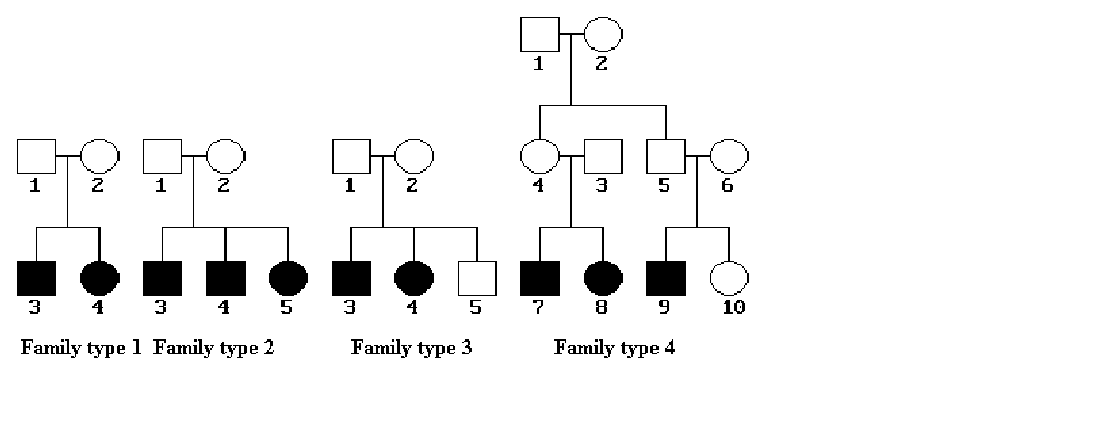
\includegraphics[width=6.2in,height=2.5in]{f4.bmp}
\caption{The four family types\label{f4}}
\end{figure}

For a normally distributed test statistic with mean 0 and variance 1 under the
null hypothesis and mean $m$ and variance $v$ under the alternative, the sample
size required based on 1-sided normal approximation for type I and type II
error rates $\alpha=0.0001$ and $\beta=0.1$ is $N=\lceil {[(3.719+1.282
\sqrt{v})}/{m}]^2\rceil$, where the ceiling function $\lceil.\rceil$ always
rounds fractional argument up by 1.  This has been used for NPL, so has been
for LOD and ALOD, as they are calculated directly without maximisation while
Central Limit Theorem would justify its use given large number of families.
For MLOD, MALOD and MFLOD the required sample sizes are calculated according to
their noncentrality parameters per pedigree.  The required sample sizes are
obtained for type I error rates $\alpha$=0.0001, 0.00001 and 90\% power.  The
noncentrality parameters for $\chi^2$ distribution with degrees of freedom of 1
and 2 are 26.76 and 29.92 for 2-sided tests (25.00 and 28.11 for 1-sided).

%The corresponding deviates are 3.09, 3.72 for normal, 10.83, 15.14 for $\chi^2$
%with degree of freedom 1 and 13.82, 18.42 for $\chi^2$ with degrees of freedom
%2.

The mean and variance of a statistic for family mixture can be obtained from
means and variances of individual families over all genotype configurations, as
$\sum_{j=1}^4 \tau_j m_j$ and $\sum_{j=1}^4 \tau_j (v_j+m_j^2) - (\sum_{j=1}^4
\tau_j m_j)^2$, where $\tau$ is the proportion of family type $j$ in the
mixture, and $m_j$ and $v_j$ are the mean and variance of a statistic for
family type $j$, respectively.

\subsection*{Simulation studies}

Empirical distributions for these statistics under the null hypothesis were
obtained via computer simulation.  Replicates are obtained from multinomial
distributions of genotype configurations given different family types and
transmission models under the null hypothesis.  The numbers of replicates are
determined by LOD and ALOD such that according to asymptotic theory, a
LOD score or a ALOD score test should have 90\% power at significance 0.0001.
Test statistics are calculated for 10,000 simulated samples in order to provide
their empirical distributions.  These distributions are compared with the
normal or $\chi^2$ distributions at the critical value for a significance
level of 0.001, to see if the tests produce correct p values.

%As an example, the means and variances for model 1 and family mixture under the
%null are -0.353, 0.281 for LOD and -0.074, 0.051 for ALOD, after
%standardisation they become 1.287, 0.908 for LOD and 0.720, 1.738 for ALOD, the
%required sample sizes for LOD and ALOD are 15 and 57, respectively.  Thresholds
%used in simulation for LOD and ALOD are thus $3.0 \sqrt{15 \times 0.281} + 15
%\times (-0.353)=0.864$ and $ 3.0 \sqrt{57 \times 0.051} + 57 \times
%(-0.074)=0.896$.

We shall illustrate the calculations with family 1, which has four possible
genotype configurations.  If the parental genotypes are (12, 34) and the first
offspring is assigned genotype 13, then the four configurations are specified
by the second offspring (13, 14, 23, 24).  We denote these configurations are
denoted as $i=1,\ldots,4$, so that the following quantities can be obtained,

$l_i$ - likelihood of linkage under a true model

$u_i$ - likelihood of no linkage

$p_i^0$ - probability of genotype configuration under no linkage

$p_i^\alpha$ - probability of genotype configuration under admixture

$p_i^1$ - probability of genotype configuration under full linkage

$lod_i$ - lod score for a given genotype configuration

$alod_i$ - admixture lod score for a given genotype configuration

\noindent
We use {\bf VITESSE} (O'Connell \& Weeks 1995; O'Connell 2001) to obtain the
quantities $\log_{10}(l_i)$ and $\log_{10}(u_i)$. Then
\begin{eqnarray*}
p_i^0 &=& 1/4 \cr
p_i^1 &=& l_i/\sum_{j=1}^4l_j=10^{\log_{10}(l_i)+M}/\sum_{j=1}^410^{\log_{10}(l_j)+M},\quad i=1, \ldots, n\cr
p_i^\alpha &=& (1-\alpha)p_k^0+\alpha p_k^1
\end{eqnarray*}
where $M$ is a large number used to avoid underflow. As usual,
$lod_i=\log_{10}(l_i/u_i)$, $alod_i=\log_{10}((\alpha
l_i+(1-\alpha)u_i)/u_i)=\log_{10}(\alpha 10^{lod_i}+(1-\alpha))$.
Further we have under no linkage
\begin{eqnarray*}
\mbox{E(LOD)}  &=& \sum_{j=1}^4p_j^0lod_j\cr
\mbox{V(LOD)}  &=& \sum_{j=1}^4p_j^0lod_j^2-[\mbox{E(LOD)}]^2\cr
\mbox{E(ALOD)} &=& \sum_{j=1}^4p_j^0alod_j \cr
\mbox{V(ALOD)} &=& \sum_{j=1}^4p_j^0alod_j^2-[\mbox{E(ALOD)}]^2
\end{eqnarray*}
and under linkage
\begin{eqnarray*}
\mbox{E(LOD)}  &=& \sum_{j=1}^4p_j^1lod_i \cr
\mbox{V(LOD)}  &=& \sum_{j=1}^4p_j^1lod_j^2-[\mbox{E(LOD)}]^2 \cr
\mbox{E(ALOD)} &=& \sum_{j=1}^4p_j^\alpha alod_j \cr
\mbox{V(ALOD)} &=& \sum_{j=1}^4p_j^\alpha alod_j^2-[\mbox{E(ALOD)}]^2
\end{eqnarray*}

Using these quantitities the required sample size at significance level of
0.0001 and 90\% power can be calculated for LOD and ALOD, which will be
used in setting their thresholds in simulations under the null hypothesis
and for calculation of MLOD, MALOD and MFLOD.  Note that under the null
hypothesis means and variances of LOD and ALOD may deviate slightly from 0
and 1, the calculation of sample sizes takes into account of this fact by
appropriate standardisation according to their means and variances under
the null.  Also note that calculations for LOD and ALOD are carried out
under true models of linkage and no linkage and we assume $\alpha=0.5$.  
The calculations of NPLpair and NPLall are similar to LOD and ALOD as they
do not need model assumption, while calculations of MLOD, MALOD, MFLOD
allow for variation of $f_1$ (by keeping prevalence $K$ constant) and
$\alpha$.  To compensate for the observation that the maximised
log-likelihood for MFLOD often deviates from the true model, a finer grids
for $f_1$ are used either around $K$, or near 0 and 1 with an exponential
degradation, and MLOD and MALOD are obtained accordingly using this grids.  
MFLOD and MALOD are obtained by modifying {\bf MFLINK}, while NPL
statistics are based on {\bf GENEHUNTER} routines {\em score\_pairs} and
{\em score\_all}.  Indeed the probabilities of genotype configurations for
family 1 can be compared to IBD distribution of affected sib pair derived
by Suarez et al (1978).  The thresholds used in simulation under the null
hypothesis for MLOD, MALOD, MFLOD and NPLs are according to $\chi^2$ and
normal deviates, respectively.

The whole procedure is implemented in a C computer program.  In the
implementation, mean $\overline X_k$ and variance $V_k$ are iteratively
calculated.  Start from $\overline X_k=X_1$ and $V_k=0$ for k=1, we have for
the $k$th iteration $\overline X_k={[(k-1)\overline X_{k-1}+X_k]}/{k}$,
$(k-1)V_k-(k-2)V_{k-1} = {X_k^2-k\overline X_k^2+(k-1)\overline
X_{k-1}^2}\equiv T$, $V_k=[(k-2)V_{k-1}+T]/{(k-1)}$.  Results are obtained
under DEC Alpha and Sun SPARC stations.


\section{Results}

Estimated sample sizes required for significance level $\alpha=0.0001$,
power $1-\beta=90\%$ at complete linkage ($\theta=0$) are given in
Table~\ref{lall}. As expected LOD needs the smallest sample size, although
sample sizes required by other statistics are not much larger.  The
patterns of sample sizes are also as expected.  Sample sizes required by
multiplicative models MM1 and MM2 may be many folds of models CR and CD.  
NPL statistics have better performance than MLOD under the multiplicative
models considered.  Both NPLs and MLOD outperform MALOD and MFLOD.

\begin{table}[h]
\caption{Estimated sample sizes required under linkage homogeneity\label{lall}}
\centering
\begin{tabular}{cccccccc}
\multicolumn{8}{c}{(100\% families are linked)}\\
\\
\hline
Model&  Family &LOD   & NPLpair&NPLall& MLOD &  MALOD & MFLOD \\
\hline
\\
CR   &  1      &18    & 20     &20    & 22   &  24    & 32\\
     &  2      &10    & 10     &10    & 13   &  15    & 17\\
     &  3      &16    & 19     &19    & 20   &  22    & 42\\
     &  4      &13    & 14     &14    & 15   &  17    & 48\\
     &  mixed  &15    & 16     &17    & 18   &  20    & 34\\
\\
CD   &  1      &50    & 52     &52    & 51   &  57    & 51\\
     &  2      &16    & 18     &18    & 20   &  22    & 20\\
     &  3      &44    & 52     &52    & 45   &  50    & 72\\
     &  4      &7     & 9      &7     & 10   &  11    & 13\\
     &  mixed  &28    & 32     &31    & 29   &  32    & 39\\
\\
MM1  &  1      &285   & 285    &285   & 312  &  348   & 311\\
     &  2      &80    & 80     &80    & 91   &  102   & 94 \\
     &  3      &245   & 312    &312   & 275  &  307   & 352\\
     &  4      &124   & 131    &132   & 145  &  162   & 280\\
     &  mixed  &173   & 192    &192   & 195  &  218   & 264\\
\\
MM2  &  1      &626   & 626    &626   & 677  &  755   & 675\\
     &  2      &199   & 199    &199   & 224  &  250   & 224\\
     &  3      &582   & 641    &641   & 636  &  710   & 1022\\
     &  4      &300   & 309    &315   & 342  &  382   & 771\\
     &  mixed  &405   & 437    &438   & 449  &  502   & 666\\
\hline
\\
\multicolumn{8}{c}{(``mixed'' refers to 50\%, 20\%, 20\% and 10\% mixture of
family types 1-4)} \\
\end{tabular}
\end{table}

Table~\ref{l50} gives estimated sample sizes under admixture with 50\% of
families demonstrating linkage.  More families are required compared to full
linkage, in a similar pattern with respective to pedigree types and disease
models.  The sample size required is more than doubled relative to complete
linkage.  ALOD will need the smallest sample size over all models and family
types.  Again NPL statistics perform very closely to but better than MLOD,
except for model CR.  Overall, all five statistics yield comparable power.

\begin{table}[h]
\caption{Estimated sample sizes required under linkage heterogeneity\label{l50}}
\centering
\begin{tabular}{cccccccc}
\multicolumn{8}{c}{(50\% families are linked)}\\
\\
\hline
Model&  Family &ALOD  & NPLpair& NPLall&  MLOD  & MALOD &  MFLOD\\
\hline
\\
CR   &  1      &74    & 92     & 92    &  84    & 94    &  119  \\
     &  2      &35    & 45     & 45    &  44    & 48    &  63   \\
     &  3      &65    & 87     & 87    &  77    & 84    &  172  \\
     &  4      &44    & 57     & 57    &  56    & 58    &  157  \\
     &mixed    &57    & 73     & 73    &  72    & 74    &  131  \\
\\
CD   &  1      &227   & 228    & 228   &  241   & 270   &  241  \\
     &  2      &79    & 80     & 80    &  88    & 99    &  88   \\
     &  3      &191   & 228    & 228   &  224   & 228   &  284  \\
     &  4      &26    & 40     & 33    &  35    & 37    &  47   \\
     &mixed    &111   & 138    & 133   &  133   & 134   &  149  \\
\\
MM1  &  1      &1139  & 1151   & 1151  &  1245  & 1390  &  1243 \\
     &  2      &305   & 315    & 315   &  345   & 379   &  357  \\
     &  3      &965   & 1258   & 1258  &  1105  & 1206  &  1376 \\
     &  4      &468   & 512    & 509   &  538   & 599   &  1008 \\
     &mixed    &663   & 764    & 763   &  755   & 841   &  1041 \\
\\
MM2  &  1      &2503  & 2515   & 2515  &  2701  & 3018  &  2703\\
     &  2      &771   & 781    & 781   &  864   & 960   &  860\\
     &  3      &2317  & 2577   & 2577  &  2514  & 2806  &  4036\\
     &  4      &1159  & 1212   & 1224  &  1288  & 1439  &  2887\\
     &mixed    &1585  & 1739   & 1740  &  1761  & 1964  &  2675\\
\hline
\\
\multicolumn{8}{c}{(``mixed'' refers to 50\%, 20\%, 20\% and 10\% mixture of
family types 1-4)} \\
\end{tabular}
\end{table}

Simulation result under the null hypothesis is shown in Table~\ref{lnull}.
Since the significant level has been set to 0.001, we expect 10 of the
10,000 replicates would yield values as extreme under the null hypothesis
(above or below this level reveals anticonservative or conservative test).  
The normal approximations by LOD and ALOD seem acceptable except for model
CR.  NPL statistics seem to be more anticonservative, especially for
family type 4 under models CR and CD, although it is less serious for MM2.  
For larger pedigrees, NPLpair seems less liberal than NPLall.  
Unsatisfactory behaviour under the null hypothesis would make it difficult
to compare power, especially for model CR.  Although model CR needs
smaller sample size than model CD, it is somewhat liberal.  MALOD and
MFLOD are too conservative overall.  This suggests we should choose MLOD
over all models.

\begin{table}[h]
\caption{Proportion of replicates (out of 10,000) simulated under the null
hypothesis reaching threshold of 0.001\label{lnull}}
\centering
\begin{tabular}{ccccccccc}
\\
\hline
Model & Family & LOD  &  ALOD &  NPLpair& NPLall&  MLOD &  MALOD & MFLOD\\
\hline
\\
CR    & 1      & 21   &  13   &  7      & 7     &  18   &  3     & 14\\
      & 2      & 25   &  26   &  41     & 41    &  10   &  2     & 6\\
      & 3      & 20   &  14   &  11     & 11    &  14   &  6     & 7\\
      & 4      & 16   &  35   &  21     & 25    &  10   &  3     & 11\\
\\
CD    & 1      & 4    &  8    &  10     & 10    &  8    &  1     & 7\\
      & 2      & 7    &  9    &  11     & 11    &  5    &  0     & 3\\
      & 3      & 5    &  10   &  10     & 10    &  10   &  3     & 5\\
      & 4      & 37   &  43   &  35     & 57    &  15   &  9     & 4\\
\\
MM1   & 1      & 5    &  6    &  5      & 5     &  2    &  0     & 1\\
      & 2      & 22   &  14   &  22     & 22    &  8    &  1     & 6\\
      & 3      & 8    &  12   &  7      & 7     &  5    &  2     & 5\\
      & 4      & 12   &  12   &  12     & 17    &  9    &  1     & 7\\
\\
MM2   & 1      & 6    &  15   &  6      & 6     &  6    &  1     & 5\\
      & 2      & 9    &  9    &  9      & 9     &  3    &  1     & 3\\
      & 3      & 8    &  13   &  12     & 12    &  5    &  5     & 5\\
      & 4      & 5    &  20   &  9      & 9     &  6    &  2     & 3\\
\hline
\end{tabular}
\end{table}


\section{Discussion}

The power of the MLOD, MALOD, NPLall and NPLpairs statistics appears to be
similar for the types of families considered, which suggests uncertain
mode of inheritance is not a serious issue for linkage analysis of genes
with minor effects.  Compared to findings of Lin et al.  (1997), NPLpair
and NPLall seem to have better performance but at the same time be more
anticonservative.  One aspect not revealed by assuming full marker
informativeness in this investigation was pointed out elsewhere
(Whittemore 1996; Kong \& Cox 1997), i.e., NPL statistics could be
conservative between markers and more appropriate statistics could be
used.  In general, to constrain the disease models by the prevalence ($K$)
may be necessary but not sufficient.  For MM1 and MM2 models, the search
over $f_1$ as in (\ref{f1}) ignores their multiplicativity and is only a
matter of convenience and may tend to underestimate the power of MLOD,
MALOD and MFLOD. This highlights the difficulty in practical data
analysis, for the disease models are often not known with certainty. It is
thus desirable to relax the recessive and dominant constraint in
(\ref{f1}), and resort to an optimisation involving the larger penetrance
space under the prevalence constraint, which would be numerically more
difficult. The poor performance of MALOD under locus heterogeneity is
likely due to the fact that penetrances and admixture parameter are
confounded in small pedigrees, an extra degree of freedom is unnecessary.

A possible limitation of the power comparisons performed here is that we
assumed that all the test statistics conformed to their asymptotic
distributions under the null hypothesis. If this is not true and some of
the test statistics give anticonservative significance level when
asymptotic distributions are used, then the power comparison may unfairly
favour these tests. Indeed, we showed that LOD, ALOD and the two NPL
statistics are somewhat anticonservative.

In principle this work can be generalised to more complicated family types
and disease models but then a complete list of all possible genotype
configurations will be computer-intensive since it could be very large.  
The generalisation of findings with respect to multiplicative models
remains to be explored.  In this study, a single fully informative marker
has been used to focus on different maximisation schemes, which enables
exact calculation of the distribution of the test statistics and to some
extent approximate multipoint analysis but will lead to two consequences.  
First, the power will be lower for marker with incomplete information.  
However, our main concern is the relative performance of these tests, we
do not expect it change dramatically. Second, the direct extension of the
finding from two-point to multipoint analysis is problematic (Risch \&
Giuffra 1992) since recombination ceases to be an effective parameter.  
Moreover, since NPL statistics assess the evidence of allele sharing among
affected relative pairs at a test position are more suitable for
multipoint analysis.

Other assumptions of this study include HWE of founder trait and marker
phenotypes, no interference, ascertainment/selection of small families (Badner
et al.  1998, 1999).


\section{Bibliographic notes}

Risch (1989) showed that for simple genetic models and nuclear family
data, ignoring heterogeneity and calculating the standard lod score tends
to be the more powerful choice unless for small linked fraction $\alpha$,
large pedigrees and small recombination fraction. Davis et al.  (1996),
Davis \& Weeks (1997) examined a variety of statistics for linkage
analysis with different genetic models and family structures and showed
that NPL had lower power compared to other methods when there was
heterogeneity in the data and when families were ascertained through two
or more affected children. MOD score is also called MMLS (maximising the
maximum lod score, or LOD score maximised over disease models) (Greenberg
1989).  In Hodge et al.  (1997), the lod score was calculated twice, once
assuming a simple dominant model and once assuming a simple recessive
model.  The maximum over the two models was then reported as result and
the type I error rate was corrected for multiple testing.  Greenberg et
al.  (1998) found the power of MMLS method to be robust, with its power
ratio to that of the simulated model greater than 0.8 over a range of
models.  Abreu et al.  (1999) compared MMLS and NPL.  They simulated 100
data sets with 20 families each, using 26 generating models:  (1) 4
intermediate models (penetrance of heterozygote between that of the two
homozygotes); (2) 6 two-locus additive models; and (3) 16 two-locus
heterogeneity models (admixture $\alpha$ = 1.0,.7,.5, and .3; $\alpha$ =
1.0 replicates simple Mendelian models).  For LOD scores, they assumed
dominant and recessive inheritance with 50\% penetrance and took the
higher of the two maximum LOD scores and subtracted 0.3 to correct for
multiple tests (MMLS-C). They compared expected maximum LOD scores and
power, using MMLS-C and NPL as well as the true model.  Since NPL uses
only the affected family members, they also performed an affecteds-only
analysis using MMLS-C.  The MMLS-C was both uniformly more powerful than
NPL for most cases they examined, except when linkage information was low,
and close to the results for the true model under locus heterogeneity.  
They still found better power for the MMLS-C compared with NPL in
affecteds-only analysis.  The results show that use of two simple modes of
inheritance at a fixed penetrance can have more power than NPL when the
trait mode of inheritance is complex and when there is heterogeneity in
the data set.  Nyholt (2000) gave a summary of critical values for lod
scores obtained under a variety scenarios including MMLS.  Further
discussion of allele-sharing statistics was given by Shih \& Whittemore
(2001).

\chapter{Case-control allelic association}

\section{Introduction}

Allelic association or haplotype analysis of a set of markers is commonly done
on samples of unrelated individuals from one or more populations (Hawley \&
Kidd 1995; Kidd et al.  2000; Schneider et al.  1997; Terwilliger \& Ott 1994;
Cox 1998; Zhao, Curtis \& Sham 2000).  These are also used to study
associations between a putative disease locus and marker(s) in samples of cases
and controls (Ott 1999; Zhao, Curtis \& Sham 2000).

When a single marker is involved, allele frequency differences between cases
and controls can be detected using a Pearson contingency table $\chi^2$ (Woolf
1955; Workman \& Niswander 1970; Sham \& Curtis 1995; Sasieni 1997; Hirotsu et
al.  2001) or a log-likelihood ratio statistic.  When more markers are
involved, it is more appropriate to use a likelihood framework based on
haplotype frequencies.  The likelihood of observing a given sample is expressed
as a function of unknown haplotype frequencies, to be maximised by numerical
method such as the EM (Expectation-Maximisation) algorithm.  This is called
gene counting since the EM steps only involve counting genes.  Some simple
scenarios including a small number of markers are illustrated in
Appendix~\ref{genecount}.  The general situation of a putative disease locus
and multiple multiallelic markers has been implemented in early version of {\bf
EH} (Xie \& Ott 1993; Terwilliger \& Ott 1994) and its successor {\bf fehp}
(Zhao \& Sham 2002).

For complex traits with uncertain disease model, it is natural to adapt
model-free statistics similar to those used in linkage analysis.  Assuming a
generalised single locus model, its parameters can be constrained to yield the
same population disease prevalence ($K$) as considered by Curtis \& Sham
(1995).  The parameters of the disease model are treated as nuisance parameters
in the likelihood function, and a likelihood ratio test is constructed in which
the likelihood under the null hypothesis is maximised over only the nuisance
parameters, while the likelihood under the alternative hypothesis is maximised
over both the nuisance parameters and the association parameters.  Similarly
the heterogeneity statistic in linkage analysis can be obtained from separate
marker-marker analyses of cases only, controls only and combined case-control
data.

It is then necessary to address issues concerning about validity and power of
such statistics.  In general, with its simple, well-known, practical and
economic advantages compared to others it is of great interest to fully
characterise and apply such design while avoiding spurious association (Long
\& Longley 1999; Risch \& Teng 1998; Devlin \& Roeder 1999; Risch 2000).  A
power analysis using the approach of Long et al.  (1997) will be given in
Chapter 7.


\subsection*{Chapter aims}

This chapter presents a power study of model-free tests in case-control
association analysis.  Similar study has been reported in Zhao \& Sham (1997),
Zhao, Curtis \& Sham (2000) but current investigation includes ordinary
contingency table $\chi^2$ and likelihood ratio tests.


\section{Methods}

Following Xie \& Ott (1993), we start by assuming a generalised single locus
model, in which a disease locus with one disease allele and one normal allele.
Under this model, the allele frequency of the disease allele $q$ and penetrance
$f_i$, $i=0,1,2$ for genotype with $i$ disease allele(s) are similarly defined
as in Chapter 2.  Contingency table Pearson $\chi^2$ (P) and LRT (G) statistics
are also used for comparison.  We consider also a haplotype model involving a
multiallelic marker B with $n$ ($n\ge 2$) alleles $B_1, B_2, \ldots, B_n$ and
allele frequencies $p_1, p_2,\ldots, p_n$.  The genotypic probabilities, based
on a subject being a case (A) or a control (U), are as follows,

\begin{eqnarray}
P(B_i B_i | A) &=& \frac{f_0 h_{1i}^2+f_1 (2h_{1i}h_{2i})+f_2 h_{2i}^2} {K}\cr
P(B_i B_j | A) &=& \frac{f_0 (2h_{1i}h_{1j})+f_1 (2h_{1i}h_{2j}
+2h_{1j}h_{2i})+f_2 (2h_{2i} h_{2j})} {K} \cr
P(B_i B_i | U) &=& \frac{s_0 h_{1i}^2+s_1 (2h_{1i}h_{2i})+s_2 h_{2i}^2} {1-K} \cr
P(B_i B_j | U) &=& \frac{s_0
(2h_{1i}h_{1j})+s_1(2h_{1i}h_{2j}+2h_{1j}h_{2i})+s_2(2h_{2i}h_{2j})}{1-K}
\label{gendist}
\end{eqnarray}
where $h_{11}, h_{12}, \ldots, h_{1n}, h_{21}, h_{22}, \ldots, h_{2n}$ are the
haplotype frequencies, and $s_i=1-f_i$.  The likelihood of the data is a
product of these probabilities, and the parameters of this likelihood function
are therefore the disease model parameters and the haplotype frequencies (Sham
1998, p159).  The maximum log-likelihood under both linkage equilibrium and
linkage disequilibrium are obtained from {\bf fehp} (Zhao \& Sham 2002).  Since
these constitute nested models, twice the difference in log-likelihood should
be asymptotically $\chi^2$ with $n-1$ degrees of freedom.  Four log-likelihood
ratio test (LRT) $\chi^2$ statistics, a heterogeneity statistic, contingency
table $\chi^2$ and log-likelihood ratio statistic are considered
(Table~\ref{brief}).

\begin{table}[h]\centering
\caption{Description of test statistics\label{brief}}
\begin{tabular}{llllllll}
\\
\hline
Statistics & Descriptions & $q$ && $f_0$&$f_1$&$f_2$\\
\hline
\multicolumn{2}{l}{Model-based}\\
T & True model & \multicolumn{4}{c}{$q$, $f_0, f_1, f_2$ are user specified}\\
R & Mendelian recessive model & $\sqrt{K}$&&0&0&1\\
D & Mendelian dominant model & $1-\sqrt{1-K}$&&0&1&1\\
F & Maximised over $f_1$ given $K$ &$q$ &&\multicolumn{4}{c}{$f_0=f_1$ or $f_1=f_2$}\\
  & (see description below)\\
\multicolumn{2}{l}{Model-free}\\
H & Heterogeneity statistic& \multicolumn{4}{c}{model not needed}\\
P & Pearson contingency table $\chi^2$&\multicolumn{4}{c}{model not needed}\\
G & LRT $\chi^2$ for contingency table&\multicolumn{4}{c}{model not needed}\\
\hline
\end{tabular}

\end{table}

These statistics are briefly described as follows.

{\bf T}:  This is the statistic one would obtain under a user-specified model,
which yields the correct population disease prevalence.

{\bf R}:  This is obtained with disease model parameters being set at Mendelian
recessive values ($q=\sqrt{K}$, $f_0=f_1=0$, $f_2=1$) in the case-control
option of {\bf fehp}.

{\bf D}:  This is obtained with disease model parameters being set at Mendelian
dominant values Mendelian penetrances ($1-\sqrt{1-K}$, $f_0=0$, $f_1=f_2=1$) in
the case-control option of {\bf fehp}.

{\bf F}:  This is obtained with disease model parameters being treated as
nuisance parameters.  The maximum likelihood is obtained from multiple runs of
{\bf fehp} with models that are constrained to produce the correct population
risk $K$ similar to {\bf MFLINK} (Curtis \& Sham 1995, see also Chapter 2),
which implies that only $f_1$ is free, and that $f_0 = f_1$, $f_2 =
1-f_1(1-K)/K$ when $f_1\leq K$, $f_2 = f_1$, $f_0 = (1-f_1)K/(1-K)$ when
$f_1>K$.  Specifically, $f_1$ is restricted to vary along the sides of the
triangle of $(0,0,1)$, $(K,K,K)$ and $(0, 1, 1)$.  Given $f_0$, $f_1$,
$f_2$, $q$ is obtained by solving $q^2f_2+2q(1-q)f_1+(1-q)^2f_0 = K$, namely
$$q=\frac{-2(f_1-f_0) + \sqrt{[2(f_1-f_0)]^2 - 4(f_0-2f_1+f_2)(f_0-K)}}
{2(f_0-2f_1+f_2)}$$ and $q=0.5(K-f_0)/(f_1-f_0)$ if $(f_0-2f_1+f_2)=0$ and 1 if
$f_2=K$.  Unlike {\bf MFLOD}, this statistic does not maximise $f_1$ in the
denominator of the likelihood ratio, the likelihood under the null is always
the likelihood assuming linkage equilibrium. To allow for an extra degree
of freedom maximising $f_1$, this should have $n$ degree of freedom.

{\bf H}:  This is a heterogeneity test in allele frequencies between cases and
controls.  As described above, the {\bf fehp} program is used three times, once
for cases alone, controls alone, and once for the cases and controls pooled
together.  In each analysis, allele frequencies are estimated and the maximum
log-likelihood calculated.  The likelihood of an individual is simply the
probability of the genotype assuming HWE.  Denoting these maximum
log-likelihoods as $l_{case}$, $l_{control}$ and $l_{combine}$, the test
statistics -$2(l_{case}+l_{control}-l_{combine}$) is asymptotically $\chi^2$
with $[(n-1) + (n-1) + (n-1)]=n-1$ degree of freedom.  The EM algorithm
requires at least two loci, but now only one marker is involved, so a
monomorphic marker is used for these individual marker-marker analyses.  This
statistic tests allele frequency differences between cases and controls
assuming Hardy-Weinberg equilibrium.

Statistics {\bf G} and {\bf P} are based on $2\times n$ contingency table in
this case; both are asymptotically $\chi^2$ with $n-1$ degrees of freedom.
Pearson $\chi^2$ statistic is more familiar while likelihood ratio test
statistic is more comparable to the model-based statistics above.  Note both G
and P use alleles rather than genotypes, so they require HWE to be valid tests
of association (Sasieni 1997).  P and G can also be based on the genotypes but
their degrees of freedom will be much larger for comparison with statistics
given above.  Hence subsequent calculations are based on allele counts.

Haplotype frequencies from Oudet et al.  (1993) on fragile X Syndrome are used
to evaluate power of model-free tests against correctly or incorrectly
specified parametric tests.  The frequencies of the seven alleles at DXS548 are
0, 42, 32, 1, 1, 29, 1 on fragile X chromosomes and 2, 117, 23, 1, 1, 15, 2 on
normal chromosomes.  The frequency of the disease allele is set arbitrarily to
be 0.001 for both R and D.  For each single gene disease models given
Table~\ref{model}, 500 replicate samples of 1,000 subjects (500 cases and 500
controls) and 500 replicate samples of 10,000 subjects (5,000 cases and 5,000
controls), are simulated in order to investigate the accuracy of the asymptotic
$\chi^2$ distribution as a function of sample size.

Five Mendelian models (Table~\ref{model}) with reduced penetrances and
phenocopies are used to simulate data in order to examine the performances of
test statistics.  They vary from simple Mendelian to recessive and dominant
models, both rare and common.  The choice of these models follows similar
argument in Chapter 2.  A minor gene model specifies a multiplicative model
with genotype relative risk of 4, as has been used earlier for Alzheimer's
(Sham \& Curtis 1995a, see also Chapter 2).

\begin{table}[h]\centering
\caption{The five genetic models\label{model}}
\begin{tabular}{lrrrcc}
\\
\hline
 Model                 & $f_0$ & $f_1$ & $f_2$ &  $q$     &   $K$\\
\hline
0 Null ($H_0$)         &   0.5 &  0.5  & 0.5   &0.5000    &0.500\\
1 Rare recessive (RR)  &     0 &    0  &   1   &0.0316    &0.001\\
2 Rare dominant (RD)   &     0 &    1  &   1   &0.0005    &0.001\\
3 Common recessive (CR)& 0.005 &0.005  & 0.5   &0.1000    &0.010\\
4 Common dominant (CD) & 0.005 &0.500  & 0.5   &0.0050    &0.010\\
5 Minor gene (MG)      & 0.050 &0.200  & 0.8   &0.1300    &0.100\\
\hline
\end{tabular}
\end{table}

The properties of each statistic under each model are investigated using
simulated samples.  The mean value of the test statistics of the replicates is
an estimator of its theoretical expectation (which is the sum of the
noncentrality parameter and degree of freedom).  This allows the noncentrality
parameter to be estimated.  Under the null hypothesis ($H_0$), the
noncentrality parameter should be 0.  A value greater than 0 implies an
increase in the false positive rate, while a value less than 0 indicates that
the test is conservative.  Under an alternative hypothesis, the non-centrality
parameter determines the power of the test.  At 5\% significance level, the
values of non-centrality parameter required for 90\% power are 17.4 and 18.3
for degrees of freedom 6 and 7, respectively.  The required sample size can be
extrapolated from the estimate of noncentrality parameter of the simulated
samples for any desired level of power.  Here the empirical means obtained from
simulated samples of size 10,000 are used as approximate estimates of
noncentrality parameters so the required samples sizes can be obtained (90\%
power at 5\% significance, assuming equal number of cases and controls).  An
exception is specifying null model ($H_0$) as in Table~\ref{model} would result
in zero log-likelihood.


\section{Results}

The results for 500 replicates of 500 cases and 500 controls are given in
Table~\ref{mf1}.  Under $H_0$, the empirical means exceed the theoretical means
(6) for R, D, and H, the reverse is true for F (7).  Interestingly, H and G are
very close to R.  While P and G compare fairly well, the mean of P as a
$\chi^2$ statistic is fairly close to its asymptotic value (6) but G tends to
be larger.  The likelihood-based statistics R, D, H are at least as good as
ordinary log-likelihood ratio statistic G, so their inflation under $H_0$ is
acceptable considering the wide use of G.  The statistics under the remaining
models provide estimates of noncentrality parameters of the associated $\chi^2$
distribtion, which can be used for obtaining sample size given certain
significance level and power (data not shown).  We expect that under
alternative hypotheses the empirical means from simulated samples of size
10,000 are approximately 10 times the corresponding values from that of size
1,000, as demonstrated below.

\begin{table}[h]\centering
\caption{Mean and standard deviation of $\chi^2$ statistics from
1,000 subjects\label{mf1}} (500 replicates of 500 cases and 500 controls)\\
\begin{tabular}{crrrrrrr}
\\
\hline
Model   &    T &      R &       D &        F &       H &       P &       G\\
\hline
$H_0$&         &   6.15 &    6.08 &     6.38 &    6.17 &    6.03 &    6.18\\%5.39
     &         &   3.33 &    3.22 &     3.42 &    3.37 &    3.22 &    3.38\\%2.80
RR   &  327.22 & 327.22 &  242.03 &   327.30 &  327.22 &  312.99 &  327.17\\
     &   33.96 &  33.96 &   23.16 &    33.98 &   33.96 &   31.83 &   33.92\\
RD   &  109.64 &  96.63 &  109.64 &   109.79 &   96.63 &   95.05 &   96.64\\
     &   19.16 &  18.02 &   19.16 &    19.23 &   18.02 &   17.46 &   18.03\\
CR   &   85.21 &  77.09 &   59.31 &    86.31 &   77.09 &   76.04 &   77.08\\
     &   18.62 &  17.87 &   13.34 &    18.81 &   17.87 &   17.40 &   17.87\\
CD   &   30.57 &  30.37 &   31.40 &    32.02 &   30.37 &   30.05 &   30.37\\
     &   10.17 &  10.21 &   10.32 &    10.43 &   10.20 &   10.04 &   10.20\\
MG   &   31.88 &  32.88 &   31.94 &    33.84 &   32.90 &   32.56 &   32.90\\
     &   10.88 &  11.14 &   10.73 &    11.30 &   11.13 &   10.98 &   11.14\\
\hline
\end{tabular}
\end{table}

The results for 500 replicates of 5,000 cases and 5,000 controls are given in
Table~\ref{mf2}.  Under $H_0$, the empirical means are slightly closer to their
theoretical values with the exception of F, which has an empirical mean of 6.24
while the theoretical mean is 7.  This indicates that the asymptotic
distribution of this statistic is closer to $\chi^2$ with 6 degrees of freedom
than $\chi^2$ with 7 degrees of freedom.  Again H and G are fairly close.

\begin{table}[h]\centering
\caption{Mean and standard deviation of $\chi^2$ statistics from
10,000 subjects\label{mf2}} (500 replicates of 5,000 cases and 5,000 controls)\\
\begin{tabular}{crrrrrrr}
\\
\hline
Model   &    T &      R &       D &        F &       H &       P &       G\\
\hline
$H_0$&         &   6.15 &    6.16 &     6.24 &    6.16 &    6.14 &    6.16\\%6.09
     &         &   3.55 &    3.56 &     3.60 &    3.55 &    3.53 &    3.55\\%3.48
RR   & 3199.29 &3199.29 & 2356.60 &  3199.29 & 3199.28 & 3063.71 & 3198.00\\
     &  111.16 & 111.11 &   77.51 &   111.11 &  111.12 &  104.43 &  110.95\\
RD   & 1041.95 & 907.50 & 1041.95 &  1041.95 &  907.50 &  895.77 &  907.54\\
     &   57.35 &  52.20 &   57.35 &    57.36 &   52.21 &   50.89 &   52.22\\
CR   &  804.95 & 716.72 &  541.28 &   805.37 &  716.69 &  710.20 &  716.74\\
     &   60.35 &  57.13 &   42.14 &    60.39 &   57.13 &   56.10 &   57.13\\
CD   &  261.98 & 252.31 &  262.59 &   262.73 &  252.31 &  251.13 &  252.35\\
     &   31.54 &  30.54 &   31.63 &    31.62 &   30.53 &   30.25 &   30.53\\
MG   &  268.79 & 270.35 &  261.75 &   270.98 &  270.23 &  269.16 &  270.26\\
     &   32.16 &  32.49 &   31.32 &    32.45 &   32.49 &   32.23 &   32.50\\
\hline
\end{tabular}
\end{table}

The required sample sizes based on 500 replicates of 5,000 cases and 5,000
controls are given in Table~\ref{mfn} (by a SAS program in Appendix).  It is
clear that rare disorders, RR in particular, require less subjects than common
disorders.  The number of subjects as required by CD is several folds that of
CR.  The number of subjects as required by major gene model is much larger than
that of rare disorder and somewhat between CR and CD considered here.

\begin{table}[h]\centering
\caption{Estimated sample sizes required for 90\% power and significance level
.05\label{mfn}} (equal number of cases and controls)\\
\begin{tabular}{crrrrrrrr}
\\
\hline
    Model&     T&      R&      D&      F&     H &   P &   G\\
\hline
     RR  &    55&     55&     74&     58&    55 &  57 &  55\\
     RD  &   167&    192&    167&    176&   192 & 195 & 192\\
     CR  &   217&    243&    322&    228&   243 & 246 & 243\\
     CD  &   665&    690&    663&    697&   690 & 693 & 690\\
     MG  &   648&    644&    665&    676&   644 & 647 & 644\\
\hline
\end{tabular}
\end{table}

No single test is uniformly more powerful over all 5 models.  T has the best
performance overall.  The power of R and H appear to be equivalent.  F is more
powerful than H in some situations.  For minor gene model, H appears to be
substantially more powerful than F.  If F is considered to have a $\chi^2$
distribution with 6 degrees of freedom, then F and H would be equally powerful
even in this situation, but then F would be slightly anti-conservative.

This shows that, when the disease model is unknown, the standard $\chi^2$ test
of homogeneity of allele frequencies (H) provides nearly optimal power,
especially for a minor gene model.  If the null distribution of the parametric
``model-free'' test (F) is accurately known, then this may be preferred to H.
Overall, the preferred test for routine use on case-control data is the
standard $\chi^2$ test of homogeneity of allele frequencies.  For data
involving related individuals, however, it is likely that parametric
``model-free'' methods will have a greater degree of superiority over
non-parametric methods.

A final observation is that for R and D models setting allele frequencies to be
0.001 other than obtaining from the correct population prevalence gives similar
results (data not shown).


\section{Discussion}

The performance of model-free statistics in case-control allelic association
analysis is investigated.  It is shown that the heterogeneity statistic is
almost as powerful as the likelihood ratio statistic taking true parameter
values of a generalised single locus model.

In view of the performance of the six statistics under the null hypothesis, the
power comparison is only considered as an approximation.  For instance,
standard errors of these statistics from Table 4 were about 0.05 ([standard
deviation]/$\sqrt{5000}$), the means of R, D, H are greater than 6, while that
of F is smaller than 7, the power calcualtion according to noncentral $\chi^2$
would be somewhat inflated for R, D, H but deflated for F, therefore the power
comparison may seem difficult.  However, similiar behaviour of the popular
statistic G offers some reassurance, as their relative performance, except F 
perhaps.  The limitaion of this study is its assumption of single locus disease 
models, which are unrealistic for complex diseases.  It further assumes the 
absence of hidden population stratification, a potential problem in real 
application.  While the study relies on asymptotic distribution theory, in 
practice Monte Carlo method should be used whenever appropriate (Zaykin et al. 
1995; Lazzeroni \& Lange 1997; Zhao, Curtis \& Sham 2000).

By including extra markers it is possible to construct a Pearson $\chi^2$
statistic and its likelihood ratio counterpart based on the haplotype table and
estimate a global LD statistic, but the Pearson $\chi^2$ statistic may often be
inflated and have poor asymptotic property.  It is common to construct such
statistics based on the genotypes of these markers.  Then test of independence
entails ``other association'' than that by the heterogeneity statistic
considered here.  These statistics for two markers has been implemented for two
markers in {\bf ASSOCIATE} (http://linkage.rockefeller.edu) and a more
comprehensive program {\bf 2LD} (Zapata et al.  2001).  The heterogeneity
statistic has been adopted both in the latest version of {\bf EH} and Fallin et
al.  (2001).  There would be concern over the validity of the chi-squared
statistics when the number of alleles become large, then empirical significance
should be used (Zhao, Curtis \& Sham 2000).  The concern over use of allelewise
versus genotypewise analysis has been extensively discussed by Sasieni (1997).

Both Koch et al.  (2000) and Fallin et al.  (2001) showed that an association
can be detected using either SNPs alone or combined with microsatellite markers
surrounding the functional locus even if the functional locus is not typed.  It
is remarkable that significant results were obtained for haplotypes defined by
loci that did not show single-locus significance.  Similar remark was made by
Longmate (2001).  It is likely that when loci influencing disease have alleles
whose impact is on the genotype level, tests using that fact may be more
powerful.  Moreover, the haplotype method does not necessarily help determine
the precise position of functional locus.  Similar note concerning fine genetic
mapping was given by Chiano \& Clayton (1998).  When parental phase is known it
can be directly used, otherwise the E-M algorithm can be applied.  While
haplotype analysis is invaluable for study of SNPs, where haplotypes will
increase the informativeness, there are theoretical and practical issues when
many loci are involved (e.g.  Zhao, Curtis \& Sham 2000).

A final note is that the case-control design should be valuable in homogeneous
or isolated populations (Shifman \& Darvasi 2001) and it is gaining more
attention (Devlin \& Roeder 1999; Risch 2000; Ghosh et al.  2000; Zhao et al.
2000; Seltman et al.  2001).


\section{Bibliographic notes}

Chapman \& Meng (1966), Guenther (1977) presented a simple formula to calculate
noncentrality parameter for alternative hypothesis of type
$h_{ij}=p_iq_j+c_{ij}/\sqrt{n}$, $\sum_{i=1}^m\sum_{j=1}^nc_{ij}=0$, i.e.,
$\lambda=\sum_{i=1}^m\sum_{j=1}^nc_{ij}^2/(p_iq_j)+\sum_{i=1}^m
c_{i.}^2/p_i+\sum_{j=1}^n c_{.j}^2/q_j$, where $c_{i.}=\sum_{j=1}^nc_{ij}$,
$c_{.j}=\sum_{i=1}^nc_{ij}$.  For two biallelic markers this is comparable to
$\lambda=2nD^2/(p_1p_2q_1q_2)$ (Weir 1996, p113), where $p$'s and $q$'s
are the allele frequencies, which is based on standard error of $D$.

Feder et al.  (1996) and Nielson et al. (1998) suggested examining departure
from HWE among affected individuals for fine-mapping of disease.  For recessive
$(\psi, \psi, 1)$ discrete model, the genotype and allele frequencies in the
population are expressed as $P(DD|A)=p_D^2/K$, $P(D|A)=p_D(p_D+\psi p_D)/K$, so
that the disequilibrium coefficient becomes
$D_{DD}=P_{DD}-p_D^2=[\psi(1-\psi)p_D^2(1-p_D^2)]/K^2$.  The quantity to
measure the departure from the Hardy-Weinberg equilibrium is
$F_D=(H_o-H_e)/(1-H_e)$ where $H_o$ and $H_e$ are the observed and expected
homozygosities, respectively.  It can be rewritten as
$F_D=[P_{DD|A}+P_{dd|A}-p_{D|A}^2-p_{d|A}^2]/(1-p_D^2-p_d^2)=[
\psi(1-\psi)p_Dp_d]/K^2$.  Association between the disease-susceptibility
allele D and a marker allele B can be expressed as $\Delta_{DB}=h_{DB}-p_Dq_B$,
where $h_{DB}$ is the frequency of haplotype carrying both alleles A and B and
$q_B$ is the frequency of marker allele $B$.  For Hardy-Weinberg
disequilibrium, $P_{BB|A}=[(1-\psi)(p_Dq_B+\Delta_{DB})^2+\psi q_B^2]/K$ and
$q_{B|A}=[\psi q_B+(1-\psi)p_D(p_Dq_B+\Delta_{DB})]/K$ so that the
Hardy-Weinberg disequilibrium coefficient among affected individuals is
$\Delta_{BB|A}=\psi(1-\psi)\Delta_{DB}^2/K^2$.  The Hardy-Weinberg departure of
Feder et al.  (1996) for the marker locus B is
$\psi(1-\psi)\Delta_{DB}^2/(K^2q_Bq_b)$ and $F_B=\Delta^2F_D$ where
$\Delta^2=\Delta_{DB}^2/p_Dp_dq_Bq_b$.  As $\Delta_{DB}$ is a function of
$(1-\theta)^{2g}$, where $g$ is the number of generations since the founding of
the mutation, $F_B$ decays approximately at a rate of $2g\theta$ with
recombination distance $\theta$ between $D$ and B.  With
$q_{B|U}=(1-\psi)[q_B-p_D(p_Dq_B+\Delta_{DB})]/(1-K)$, the commonly used LD
measure (Bengtsson and Thomson 1981, Lehesjoki et al.  1993),
$p_{excess}=(q_{B|A}-q_{B|U})/(1-q_{B|U})$ is
$$p_{excess}=\frac{(1-\psi)p_D\Delta_{DB}}{K(1-K)[q_B+(1-\psi)p_D\Delta_{DB}/(1
-K)]}$$ which is only proportional to $\Delta_{DB}$ and less sensitive than
$F_B$.  For a general disease model with multiallelic susceptibility locus and
a marker locus $B$ with $m$ allele, define $f_{rs}$ to be the ``apparent''
penetrance of genotype $D_rD_s$, so that $K=\sum_r\sum_sf_{rs}p_rp_s$, the
marker allele frequencies among the affecteds and unaffecteds are
$q_{i|A}=q_i+\delta_i/K$, $q_{i|U}=q_i-\delta_i/(1-K)$ and
$$p_{excess_i}=\frac{\delta_i}{K(1-K)[(1-q_i)+\delta_i/(1-K)]}$$ where
$\delta_i=\sum_r\sum_s p_s f_{rs}\Delta_{ri}$ and $\Delta_{ri}=h_{ri}-p_rq_i$.
The Hardy-Weinberg disequilibrium coefficients are
$\Delta_{ii|A}=h_{ii|A}-q_{i|A}^2=(K\delta_{ii}-\delta_i^2)/K^2$,
$\Delta_{ij|A}=h_{ij|A}-2q_{i|A}q_{j|A}=2(K\delta_{ij}-\delta_j\delta_j)/K^2$
and $\delta_{ij}=\sum_r\sum_s f_{rs}\Delta_{ri}\Delta_{sj}$.  A contingency
table $\chi^2$ can be built up using $n$ cases and $n$ controls as
$\chi_{CC}^2=4n\sum_i(\tilde p_{i|A}-\tilde p_{i|U})^2/(\tilde p_{i|A}+\tilde
p_{i|U})$, where $\tilde p_{i|A}$ and $\tilde p_{i|U}$ are the sample
frequencies of the marker, $\chi_{CC}^2$ has $\chi^2_{m-1}$ distribution under
the null hypothesis of no association and $\chi^2_{m-1}(\delta_{CC})$
distributed under the alternative, where
\begin{eqnarray*}
\delta_{CC}&=&4n\sum_i\frac{(q_{i|A}-q_{i|U})^2}{q_{i|A}+q_{i|U}}\cr
            &=&4n\sum_i\frac{\delta_i^2}{K^2(1-K)^2[2q_i+(1-2K)\delta_i/K(1-K)]}
\end{eqnarray*}
Similarly a Hardy-Weinberg disequilibrium test $\chi^2_{HW}$ with
$m(m+1)/2-(m-1)-1=m(m-1)/2$ degree(s) of freedom can be established.  The
noncentrality parameters for the two tests $\delta_{CC}$ and $\delta_{HW}$ are
given in Nielson et al (1998).  They noted that if the penetrances are regarded
as genotypic values, much of the theory can be applied to study of quantitative
traits (Nielsen and Weir 1999, 2001).

Zaykin et al.  (1995) describe simulation procedure to examine power of
haplotype analysis using unrelated individuals.  Mckeigue (2000) gave the
information loss in case-control design relative to family design.  Toivonen et
al.  (2000) discussed data mining.

% 29-06-00 as new chapter by upgrade report
% pending for further literature review 11/12/00
% 21/9/2001, 16/10/2001, 28/11/2001 revised

\chapter{Marker characteristics and fine mapping}

\section{Introduction}

The importance of marker characteristics in both linkage and association
analysis is now well recognised.  For example, when a parent passes a gamete
to an offspring, a recombination may occur in the parent only if the parent is
heterozygous at two joint loci.  Ott (1992) examined the sample size necessary
to characterise a marker and the effects of wrongly assuming equal allele
frequencies to linkage analysis.  Terwilliger et al.  (1992) focused on the
relative importance of marker heterozygosity and intermarker distance and
showed that high marker density may be a good substitute for low marker
heterozygosity.  Kruglyak (1997) investigated how many polymorphic and densely
spaced biallelic markers are needed for extraction of most of the mode of
inheritance information as compared to microsatellite markers.  Kruglyak (1999)
used coalescent theory and computer simulation to examine the extent to which
LD can extend in the context of genome screen and using SNPs.

Of particular interets is the advantage and disadvantage of SNPs and dense maps
over traditional markers in fine mapping.  Ott \& Rabinowitz (1997), Chapman
\& Wijsman (1998) both considered the effect of marker polymorphism on
mutation detection assuming single ancestral mutation.  Ott \& Rabinowitz
(1997) found that greater marker heterozygosity results in increased power
to detect linkage disequilibrium. A similar conclusion was reached by Chapman
\& Wijsman (1998), that multiallelic markers always have more power to detect
LD than biallelic markers.  It is desirable, however, multiple mutations can be
incorporated.

\subsection*{Chapter aims}

This chapter uses a simple deterministic model to investigate the effect of
marker polymorphism on the power of fine mapping.  The simple population
genetics model incorporates multiple ancestral mutations.  Under this model,
the effect of marker polymorphism on the power to detect linkage disequilibrium
due to multiple mutations is examined for several scenarios.  Some results of
this investigation are reported in Sham, Zhao \& Curtis (2000).


\section{Methods}

We begin with the simplest assumption that current disease chromosomes are due
to multiple ancestral mutations at a single marker locus at generation $g$.  We
assume the disease locus is recombination rate $\theta$ from the marker.  We
also assume that the marker locus have $n$ alleles, with frequencies $\pi_j,
j=1, \ldots, n$ in the population, so that there are at most $m$ mutations at
an allele and $n^m$ possible patterns of mutations in total.  Let $d_i=1,
\dots, m$ be the specific pattern of each of these $n^m$ enumerations, with a
non-zero value indicating a mutation at that allele and their counts
accumulating to $c_j$, so that marker allele frequency at the disease-carrying
chromosome at generation 0 is $f_j=c_j/m$, $j=1, \ldots, n$.  Under random
mating and nonoverlapping generations, the expected frequencies of the marker
alleles among chromosomes containing a disease mutation at generation $g$ are
obtained via the following basic relation
\begin{eqnarray}
f_j^{(g)}=f_j(1-\theta)^g+\left[1-(1-\theta)^g\right]\pi_j\label{eqn1}
\end{eqnarray}
i.e., the expected frequencies for the marker chromosome at generation $g$
is due to chromosomes that remain intact with the founder mutations and those
experienced at least one recombinations.  The allele frequencies discrepancy
between the disease chromosome and chromosomes in the population can be
measured by Pearson $\chi^2$ and likelihood ratio test statistics as follows.
\begin{eqnarray}
\chi_i^2 &=& N\sum_j\frac{(\pi_j-f_j^{(g)})^2}{\pi_j+f_j^{(g)}}\label{eqn2}
\end{eqnarray}
and
\begin{eqnarray}
l_i &=& 2N \sum_j\left[\pi_j\ln \pi_j+f_j^{(g)}\ln
f_j^{(g)}-(\pi_j+f_j^{(g)})\ln\frac{\pi_j+f_j^{(g)}}{2}\right]\label{eqn3}
\end{eqnarray}
for $i=1, \ldots, n^m$ and $N$ is the appropriate sample size. Asymptotically
$\chi_i^2$ and $l_i$ would have noncentral $\chi^2$ distribution with degree
of freedom $n-1$, and noncentrality parameters $\chi_i^2$ and $l_i$
respectively.

The appropriate area $s_i$ is calculated as the power estimate from these
two distributions that exceeds the critical value set by the global
$\alpha$ value, the type I error under the null distribution of $\chi^2$.
Denote $w_i=\prod_j \pi_j^{c_j}$,$i=1,\ldots,n^m; j=1, \dots, n$ the
multinomial probability associated with the $i-th$ of the $n^m$
enumerations, we can get an overall estimate of the power by $\sum_i
w_is_i$, $i=1,\ldots,n^m$. The estimate of $N$ can be iteratively refined
to achieve predefined power. In practice to enumerate all the $n^m$
possibilities is quite slow so we can set a number of values that are
interesting to us and get their overall estimates of power. The minimum
and maximum of $\chi_i^2$ and $l_i$ can also be recorded for each
mutation. The $n^m$ possibilities are enumerated using a recursive algorithm.

Two sets of allele frequencies are examined for markers with alleles varying
from 2 to 15, which represents fairly common polymorphisms.  In the first
scheme each allele has frequency $\pi_j=1/n$ for $j=1, \ldots, n$, so the
marker heterozygosity is easily calculated as $1-\sum \pi_j^2=1-1/n$.  In the
second scheme different alleles follow a geometric relationship,
$p_1=(1-r)/(1-r^n), \pi_j=\pi_{j-1}r, j=2, \ldots, n$, the marker
heterozygosity is $1-(1+r^n)/(1+r)p_1=[2r/(1+r)][(1-r^{(n-1)})/(1-r^n)]$.  By
setting $r=0.5$ here allele 1 has the highest frequency 0.67 for biallelic
marker and 0.5 for marker with 15 alleles, while the marker heterozygosity
increases from 0.44 to 0.67.  A proportion of $r=9/11\approx 0.82$ is used so
that allele 1 has the highest frequency 0.55 for biallelic marker and 0.19 for
15-allele marker while the marker heterozygosity increases from 0.50 to 0.89.

The following combinations are examined for 1 to 5 mutations:  the generation
$g=20$, 50 and 80, the recombination fractions $\theta=0.005$ and 0.05.  It is
expected that combinations such as $g=50$, $\theta=0.005$ and $g=50$,
$\theta=0.05$ will give comparable results to $g=500,\theta=0.0005$ and $g=500,
\theta=0.005$.

The entire calculation is done by a C program calling up a number of
subroutines:  subroutine {\em digit} for the recursive enumeration, Fortran
routines to calculate central and noncentral $\chi^2$ distribution functions
and noncentrality parameters, unidimensional optimisation procedures {\em
fibonacci} and {\em fmin} to determine the required sample size for a given
type I error rate and power.  Subroutines {\em digit}, {\em fibonacci}, {\em
fmin} are listed in Appendix B.  Fortran routines are based on algorithms
published in Applied Statistics (AS91, AS170, AS245, AS275, available from
http://lib.stat.cmu.edu).


\section{Results}

Table~\ref{table4_1} shows required the sample size based on the exact
calculation.  In general, the likelihood ratio test statistic exhibits more
power (data not shown) than Pearson $\chi^2$.  As the number of mutations
increases, the effect of number of alleles is more pronounced.

\begin{table}[h]
\caption{Required sample sizes for $\alpha=0.001$ and $1-\beta=0.9$ over
$g=20, 50, 80$ and $\theta=0.005, 0.05$\label{table4_1}}
\end{table}
%\oddsidemargin=-0.5cm
%\evensidemargin=-1.5cm
\begin{alltt}
               20                    50                         80
       0.005      0.05       0.005        0.05         0.005         0.05

mutation=1
2    41   61   315   521    59   90   7000  12404    83  130   153301  273655
3    30   49   207   396    43   71   4166   9138    59  102    88030  200080
4    27   47   170   372    38   68   3132   8435    51   96    64423  184002
5    26   48   152   372    36   69   2594   8373    48   97    51989  182552
6    26   49   142   380    35   71   2262   8557    46  100    44229  185929
7    25   51   135   393    34   73   2037   8813    45  103    38891  191671
8    25   53   131   407    34   76   1874   9124    45  107    34973  198183
9    26   54   128   421    34   78   1752   9427    45  111    31966  204930
10   26   56   127   435    34   81   1656   9734    45  114    29579  211906
11   26   58   125   448    35   83   1579  10033    45  118    27635  218092
12   26   60   125   461    35   86   1516  10321    46  121    26017  224348
13   27   61   124   473    35   88   1464  10598    46  125    24659  230376
14   27   63   124   485    36   90   1421  10865    46  128    23476  236202
15   27   64   124   497    36   93   1386  11123    47  131    24560  241776

mutation=2
2     a  348     a   500     a  463      a  44655     a  625        a  962221
3    70  105   597   806   103  151  14000  18118   149  213   313316  394666
4    47   84   364   649    68  121   8157  14590    96  171   177318  317607
5    39   80   284   614    56  115   6018  13761    78  162   128958  299360
6    36   80   243   615    50  115   4901  13744    70  162   103561  298950
7    34   82   219   629    47  118   4208  14042    65  166    87774  305250
8    33   85   203   647    45  121   3735  14469    62  171    76781  314506
9    32   87   191   669    44  125   3387  14954    59  177    68822  325265
10   32   90   183   691    43  130   3122  15440    58  183    62571  335538
11   31   93   177   713    43  134   2914  15926    57  188    57733  346085
12   31   96   172   733    42  137   2745  16397    56  194    53700  356640
13   31   98   168   754    42  141   2606  16857    56  199    50318  366325
14   31  101   165   774    42  145   2488  17303    56  204    47487  375945
15   31  103   163   793    42  149   2388  17724    56  209    45054  385233


mutation=3
2   416    b  2704     b   566    b  58884      b   768    b  1278369       b
3     c  159     c  1287     c  229      c  31032     c  325        c  688633
4    90  114   792   908   133  164  19342  21294   193  233   426784  469190
5    60  104   490   821    88  150  11371  19050   125  212   250193  418463
6    50  103   382   806    72  148   8917  18605   101  209   185013  408269
7    45  104   325   817    64  150   6968  18815    89  212   149953  412510
8    42  107   289   838    59  154   5991  19298    81  218   127695  422995
9    40  111   265   864    56  159   5312  19893    76  225   112179  436012
10   38  114   248   892    53  164   4811  20541    73  232   100678  449925
11   37  118   235   919    52  169   4424  21166    70  239    91740  463938
12   37  121   225   946    51  174   4116  21796    69  246    84601  478114
13   36  124   217   973    50  179   3865  22406    67  252    78743  491271
14   36  127   210   998    49  183   3658  23011    66  259    73836  504429
15   36  130   205  1022    49  188   3481  23578    65  265    69670  516839

mutation=4
2     d 1147     d  7608     d 1564      d 168285     d 2131        d 3666858
3   402  349  2549  2066   538  461  51458  43946   721  612  1111038  949769
4   145  149  1126  1140   209  213  25214  25979   296  300   600000  567967
5    94  128   812   987   138  184  19767  22497   199  259   438705  491914
6    69  124   561   953   100  178  13159  21686   143  250   300000  474056
7    58  125   453   958    84  179  10500  21796   118  252   200000  476267
8    52  128   390   980    75  183   8948  22282   105  257   185964  486771
9    48  131   349  1008    69  188   7465  22913    96  265   160620  500750
10   46  135   320  1038    65  194   6668  23618    90  273   142447  516039
11   44  139   299  1069    62  199   6066  24324    85  281   128703  531745
12   43  143   283  1100    60  205   5594  25035    82  289   117840  547029
13   42  147   269  1130    58  210   5213  25723    80  297   109060  562118
14   41  151   259  1158    57  216   4900  26377    78  304   101786  576605
15   40  154   250  1186    56  221   4634  27019    76  311    95649  590692


mutation=5
2  1113 1841  7137 11455  1507 2476 155053 245369  2038 3328  3365250 5310142
3   482  532  3303  3408   663  720  73968  73848   910  975  1616146 1601564
4   370  192  2178  1428   492  305  44962  32560   655  380   964316  713259
5   120  156  1929  1176   173  272  20801  26795   244  311   452149  586413
6    91  147   726  1115   132  222  16362  25343   188  295   355886  554258
7    74  147   500  1112   107  210  14000  25253   153  294   300000  552080
8    64  150   499  1133    93  214  11191  25723   131  300   254320  562118
9    58  154   440  1163    84  219  10500  26395   118  308   200000  577296
10   54  158   398  1197    77  225   8986  27181   108  317   184955  593975
11   51  163   367  1233    73  232   7765  27980   102  326   166406  611709
12   49  167   344  1269    70  239   7121  28783    97  335   151890  629200
13   48  172   325  1303    67  245   6605  29570    93  344   140077  646404
14   46  176   310  1336    65  251   6180  30339    90  353   130371  663337
15   45  180   298  1368    63  257   5824  31072    87  362   122251  679534

The maximum attainable powers for these cases are (a) 0.500, (b) 0.778, (c)
0.556 and (d) 0.625. See text for more details.
\end{alltt}

Several observations can be made.  Firstly, for the three generations
considered here the decay of linkage disequilibrium is not so remarkable for
$\theta=0.005$ compared to $\theta=0.050$.  Secondly, power usually increases
with the number of alleles, so the sample size required for biallelic marker
may be ten times or more for marker with fifteen alleles.  The power seems to
attain its maximum at about 10 alleles.  Finally, a larger sample size is
required for more mutations.  For $g=20$ generations this increase is very slow
but for $g=50$ and $\theta=0.05$, the increase is roughly proportional to
number of mutations.  Moreover, the log-likelihood ratio statistic provide
slightly larger power than Pearson $\chi^2$.

There are four special cases; the mutation-allele combinations 2-2, 3-3 and 4-2
under equal allele frequencies when there is one mutation in each allele, and
3-2 under unequal allele frequencies when there are two mutations occurring in
the more frequent allele and one mutation occurring in the less frequent
allele.  In such cases, the noncentrality parameters reduce to zero, so it is
impossible to achieve more power than certain magnitude by the statistics
proposed here.  Suppose the number of instances with zero noncentrality
parameter is $n_0$, the maximum attainable power is predicted as follows,
\begin{eqnarray}
1-n_0(1-\alpha)w_i\label{eqn4}
\end{eqnarray}
where $\alpha$ is the type I error rate, $w_i$ is the probability weight.

For equifrequent marker, according to equation (\ref{eqn1}), the
three combinations each result in the same expected allele frequencies as
observed in $n_0$=2, 6 and 6 instances, respectively. Since the weight
$w_i$ is $1/n^m$, the optimal powers are therefore 0.500, 0.778 and 0.625.
Under unequal allele frequencies the weight is $4/27$ and there are
$n_0=3$ such instances so the optimal power is 0.556.


\section{Discussion}

Fine mapping of disease mutation depends on both mutation-marker distance and
age of mutation.  We have in addition quantified the effect of number of
mutations and number of alleles.  When $\theta\ll 0.5$, equation (\ref{eqn1})
is roughly a linear function of $g\theta$, so that for old mutations to be
detected, the marker has to be fairly close.  Even in population isolates,
recent mutations are less interesting than those brought in by founders.  This
has important implications with respect to the recent attention to SNPs (Guo \&
Lange 2000).

We only examined two simple scenarios, one assuming equal allele frequencies
and one with a geometric decrease between alleles.  Results for 20 and 80
generations not reported in Sham, Zhao \& Curtis (2000) are also included.
Equal allele frequency tend to have greater power, as noted by Ott (1992) in
the context of linkage analysis.  The optimal number of alleles won't
necessarily be large for detecting specific number of mutations although the
reality may be more complicated.  We do not consider actual mutation mechanism
such as single and multiple step mutations (Farrall \& Weeks 1997).  Many
factors such as selection or population growth rate would affect the result.
An obvious note from Chapman \& Wijsman (1998) is that when choosing between
markers with the same heterozygosity and different number of alleles, the one
with fewer alleles will be more powerful.

The current model is simple to interpret and easy to apply to multiple
mutations.  Ott \& Rabinowitz (1997), Chapman \& Wijsman (1998) used simple
deterministic models and assumed that a single founder of the population was
responsible for a mutation at the disease locus at $g$ generations ago, and a
marker locus with recombination rate $\theta$ with the disease mutation was
used, which had $n$ alleles each with frequencies $\pi_1, \ldots, \pi_n$.  Ott
\& Rabinowitz (1997) assumed that a priori any member of the population was
equally likely to be the founder so the probability that mutation coupled with
$i$-th allele was $\pi_i$.  After $g$ generations a proportion
$\rho=1-(1-\theta)^{(g-1)}$ had undergone at least one recombination between
the disease locus and the marker locus.  Also among the proportion of
chromosomes in which the disease mutation undergone a recombination, the
distribution of marker alleles was not different from that of general
population, which implied there were random mixing and negligible genetic
drift.  Let $O_i$ denote the number of chromosomes in the sample with the
$i$-th allele, and $E_i=N\pi_i$ the expectation under the null hypothesis of no
disequilibrium, a Pearson $\chi^2$ statistic $\sum_{i=1}^n{(O_i-E_i)^2}/{E_i}$
can be constructed and referred to $\chi^2$ distribution with $n-1$ degrees of
freedom.  If the original mutation was in coupling with a fixed but arbitrary
allele $i^\star$, so that the prevalence of the $i^\star$-th allele in the
population of chromosomes containing the original mutation was
$(1-\rho)+\rho\pi_{i^\star}$, the noncentrality parameter became
$N(1-\rho)^2(\pi_{i^\star}^{-1}-1)$, or $N(1-\rho)^2(n-1) \equiv
N(n-1)(1-\theta)^{2(g-1)}$ with equal allele frequencies, where $N$ is the
sample size.  Setting $N=100$ and assume equal allele frequencies, they
conducted 3,600 simulations for $g=20, 50, 80$ and $n=2, \ldots, 10$.  In
Chapman \& Wijsman (1998), a mutation introduced into the population had a very
small frequency $r$, then the marker allele frequencies in the disease
mutation-carrying chromosomes and the normal chromosomes were
$$x_j^{(g)}=\cases{[1-(1-\theta)^g]\pi_j & $j=1,\ldots,i-1,i+1,\ldots,n$\cr
(1-\theta)^g+[1-(1-\theta)^g]\pi_j & $j=i$} $$ and $y_j^{(g)}\approx\pi_j,
~j=1,\ldots,n$, where $i$ was the index for initial mutation on a background of
allele $i$.  They examined several disease models.  In the recessive case, the
observed marker allele frequencies in cases and controls were roughly
$x_j^{(g)}$ and $y_j^{(g)}, ~j=1,\ldots,n$; in the dominant case,
$0.5(x_j^{(g)}+\pi_j)$ and $y_j^{(g)}, ~j=1,\ldots,n$; for mixture model with
any other fractions.  The same $\chi^2$ is constructed but Chapman \& Wijsman
(1998) assumed marker polymorphism proceed the disease mutation and an
expected $\chi^2$ statistic was obtained from the weighted average of the
$\chi^2$ for each allele.  Their considerations were mainly for biallelic and
multiallelic markers with equifrequent alleles.  Equation (\ref{eqn1}) is
comparable to Ott \& Rabinowitz (1997) for one mutant allele.  Since
$(1-\theta)^g\approx 1-\theta g$, we have $\rho\approx\theta g$, their basic
relation becomes $1-\theta g + \theta g \pi_{i^\star}$.  By equation
(\ref{eqn1}), it would be $(1-\theta g+\theta g\pi_j)$, and we evaluate $w_j$
by enumeration instead of by simulation.  Chapman \& Wijsman (1998) also had
similar forms.


\section{Bibliographic notes}

Consider a specific haplotype $(A_i,B_j)$ formed by loci $A$ and $B$ whose
alleles are indexed by $i$ and $j$.  Suppose that start from generation 0, all
individuals are produced by random mating.  Then the probability of haplotype
$(A_i,B_j)$ in generation 1 is $h_1(A_i,B_j)=(1-\theta)h_0(A_i,B_j)+\theta
P(A_i)P(B_j)$, where $\theta$ is the recombination rate between $A$ and $B$,
and $h_0(A_i,B_j)$ is the probability of $(A_i,B_j)$ in generation 0.  The
disequilibrium in generation 1 is
$\Delta_1=h_1(A_i,B_j)-P(A_i)P(B_j)=(1-\theta)\Delta_0$, where $\Delta_0$ is
the disequilibrium in generation 0.  After $g$ generations, the disequilibrium
is $\Delta_g=(1-\theta)^g\Delta_0$.  For loci that are unlinked ($1-\theta$ =
1/2), the equilibrium is reached quickly; for example, $(1/2)^{10}=1/1024$.  In
contrast, for tightly linked loci the disequilibrium decays very slowly; for
example $(1-\theta)^{10}>1/3$ for $\theta=0.1$.  In the case of tightly linked
loci $(1-\theta)^g\approx 1-g\theta$, and $\theta g$ dominates the decay of
disequilibrium.  Similar result can be obtained for multiple loci (Geiringer
1944; Bennett 1954).  For simplicity subscripts of loci A, B and C are dropped
and the expressions become $h_{g+1}(AB)=(1-\theta)h_g(AB)+\theta P(A)P(B)$,
$\Delta_g(AB)=h_g(AB)-P(A)P(B)$,
$\Delta_g(AB)=\theta\Delta_{g-1}(AB)=(1-\theta)^g\Delta_0(AB)$.  For three loci
A, B and C, we have
$h_{g+1}(ABC)=(1-\theta_{AB})(1-\theta_{BC})(1-\theta_{AC})h_g(ABC)
+\theta_{AB}(1-\theta_{BC})P(A)h_g(BC)+\theta_{AB}(1-\theta_{AC})P(B)h_g(AC)
+\theta_{AC}(1-\theta_{AB})P(C)h_g(AB)$, and if we define
$\Delta_g(ABC)=h_g(ABC)-P(A)\Delta_g(BC)-P(B)h_g(AC)-P(C)\Delta_g(AB)
-P(A)P(B)P(C)$, then
$\Delta_g(ABC)=(1-\theta_{AB})(1-\theta_{BC})(1-\theta_{AC})\Delta_{g-1}(ABC)
=[(1-\theta_{AB})(1-\theta_{BC})(1-\theta_{AC})]^g\Delta_0(ABC)$.

H\"{a}stbacka et al.  (1992) noted that the best chance of success with allelic
association mapping is when most of the disease chromosomes in the population
descend from a single ancestral mutation and the mutation is old enough to
allow recombination to break up the ancestral haplotype, but not so old that
the maintained neighbourhood around the disease locus is too small to be easily
detected.  These conditions often hold for isolated founder populations that
are not very old.  If one can identify an isolated human population in which a
significant fraction of affected individuals have inherited the predisposing
allele from a common ancestor, one can exploit the tremendous power of LD
mapping (allelic association mapping).  The resolution of recombinational
mapping in a limited family series can be greatly improved, even in the case of
relatively recently expanded genes in isolated founder populations, for disease
chromosomes that descend from the same ancestral mutation should share a common
haplotype in a neighborhood of the disease locus, reflecting the haplotype on
the ancestral chromosome on which the mutation occurred.  De la Chapelle (1993,
1998) gave many practical examples.

Several methods were proposed to formulate expected haplotype frequencies
assuming affected individuals are descended from a common founder, especially
for Mendelian disorders in population isolates such as Finland (Terwilliger
1995; Jorde 1995; Kaplan 1995; Devlin et al.  1996; Xiong \& Guo 1997; Guo
1997; Rannala \& Slatkin 1998; Lazzeroni 1998).  These developments rely on
simplicity of the underlying population genetics model.  The methods of both
Kaplan et al.  (1995) and Devlin et al.  (1996) would only be effective when a
single haplotype currently has a high frequency in disease chromosomes.
Terwilliger's method combines the likelihood ratio statistics from separate LD
analyses of each marker and does not use all the information in a haplotype.
Service et al.  (1999) evaluates a LD-mapping method for genome screening in
founder populations which make direct use of haplotype information assuming
affected individuals are related to a common founder.  Rannala \& Slatkin
(1998) showed this method will produce maximum likelihood estimate when
genealogy of affected individuals is of ``star'' type, which implies
individuals are related only through one common ancestor.  Other works include
Thompson \& Neel (1997), Lazzeroni (1998), Graham \& Thompson (1998, 2000),
McPeek \& Strahs (1999), MacLean et al.  (2000), Morris et al.  (2000), Wright
et al.  (2000).  Clayton (2000) \& Lazzeroni (2001) gave comprehensive reviews
of these works. A coalescent approach to study LD between SNPs was also
conducted by Z\"{o}llner \& von Haeseler (2000). A Bayesian approach has been
adopted by Liu et al (2001).

A procedure developed by Waller et al.  (1995) for evaluating power is
described here.  Consider the distribution function of $Z=\sum_{k=1}^na_kY_k$,
where $a_k, k=1,\ldots, n$ are the weights taking real values, and $Y_k,
k=1,\ldots,n$ are independent non-central chi-squared random variables with
$n_k$ degrees of freedom and noncentral parameters $\delta_k$, for
$k=1,\ldots,n$.  The distribution functions of $Y_k$ and $Z$ do not have closed
form, but their characteristic functions do.  From above the characteristic
function for $Z$ is $\phi_Z(t)=\prod_{k=1}^n\phi_{Y_{k}}(a_kt)$.  Also
$E(Z)=\mu=\sum_{k=1}^na_k(n_k+\delta_k)$ and
$V(Z)=\sigma^2=\sum_{k=1}^na_k^2(n_k+2\delta_k)$.  We scale $Z$ to obtain
$Z'=(Z-\mu)/\sigma$, whose characteristic function is given by the formula
$\phi_{Z'}(t)=\exp(-it\mu)\phi_Z(t/\sigma)$, the following inversion formula
can be utilized to obtain the cumulative distribution function.
$$F_Z(z)=\frac{1}{2}+\frac{\mu
z}{2\pi}-\sum\limits_{n=1-H}^{H-1}\frac{\phi_Z(\eta n)}{2\pi in}e^{-i\eta nz},
\quad n\neq 0$$ where $\eta$ is chosen to ensure the range of $F_Z(z)$ is fully
represented, i.e., the values of $F_Z(z)$ include both 0 and 1.  $H$ is chosen
to define the $(2H-1)$ points where the cumulative distribution function is
estimated.  The values for $z$ may be chosen as the Fourier frequencies, that
is $z_j=(2\pi(j-H)/2\eta(H-1)))$ for $j=1,\ldots,2H-1$.  Thus the sum can be
efficiently calculated using FFT.

\chapter{Computer simulation methods}

\section{Introduction}

Common diseases such as coronary heart disease have a complicated aetiology
which involves, among other things, genetic heterogeneity, epistasis,
pleiotropy and gene-environmental interaction, which underlies most theoretical
explorations.  For example, the RFA proposal for GAW 12 problem II delineated
such a system in which gene and environmental effects operate together on
disease susceptibility, and the major etiological components underlying the
system are simplified into five individual quantitative traits.  Nevertheless a
particular feature often overlooked by most such computer programs is LD.

Computer simulation can also be used for practical problems.  Perhaps the most
established application is power analysis of a linkage study via computer
programs {\bf SLINK} and {\bf SIMLINK}.  Given certain family structures and
genetic markers, simulation-based statistics are obtained by generating
replicates of the observed families structures conditioning on available
phenotype information.  Assuming that each replicate occurs with equal
probability, expected lod score is simply the average of lod scores of all
replicates.  This quantity at the true recombination value is designated as
ELOD.  The maximum of expected lod score (MELOD) over different recombination
values and the expected maximum lod score (EMLOD) can also be obtained.  MELOD
may not be ELOD if the estimated recombination value is inconsistent due to
sampling schemes or the wrong assumption of parameter values.  EMLOD is an
average of the maximum lod scores obtained in each replicate.  EMLOD of a
pedigree conditional on the heterozygosity/homozygosity status of each pedigree
member provides means of identifying pedigree member(s) whose marker status
have a strong impact on the linkage information provided by the pedigree, which
yields a large difference in the EMLOD for his/her pedigree depending on
whether or not (s)he is marker heterozygous.  By definition ELOD $\le$ MELOD
$\le$ EMLOD (Terwilliger \& Ott 1994; Ott 1999).


\subsection*{Chapter aims}

This Chapter highlights two scenarios of computer simulation.  First, a general
procedure for simulating oligogenic trait, taking into account LD, is
introduced.  The disease model incorporates major gene effects as well as
polygenic and environmental effects with genetic loci in linkage equilibrium or
disequilibrium.  This has been used to study power for a linkage disequilibrium
problem (unpublished data).  Second, statistical power analysis using computer
simulation is applied to two examples of homozygosity mapping (Smith 1953;
Lander \& Botstein 1987).


\section{Methods, implementations and results}

\subsection*{Simulation of oligogenic traits}

A genetic model incorporating major gene, polygenic and environmental effects
is as follows:
\begin{eqnarray}
\mathbf{x}=\mathbf{g}+\mathbf{p}+\mathbf{c}+\mathbf{e}
\end{eqnarray}
where $\mathbf{x}$ is a multivariate trait ($x_i,i=1,...,NTRAIT$), a result of
additive effects of major loci $\mathbf{g}$
 ($g_j,j=1,...,NMG$), polygenic effects $\mathbf{p}$
 ($p_k,k=1,...,NPG)$, common environment $\mathbf{c}$
 ($c_l,l=1,...,NCE$) and unique environment $\mathbf{e}$
 ($e_m,m=1,...,NUE$). The variables $\mathbf{g}, \mathbf{p}, \mathbf{c},
\mathbf{e}$ are collectively referred to as causal components of the trait.
The $NMG$ major loci are a subset of $NLOCI$ loci for which the order of loci,
their recombination fractions ($\theta_1,\theta_2,...,\theta_{NLOCI-1}$), the
number of alleles and allele frequencies of them are specified.  The meaning of
some model constants are summarised in Table~\ref{simcons}.

\begin{table}[h]
\centering
\caption{Some model constants\label{simcons}}
\begin{tabular}{ll}
\\
\hline
Constants & meaning\\
\hline
$MAXFAM$ & maximum \# of families\\
$MAXIND$ & maximum \# of individuals within a family\\
\\
$MAXLOCI$ & maximum \# of loci\\
$MAXALLELES$ & maximum \# of alleles at each locus\\
$NTRAIT$ & \# of traits\\
$NLOCI$ & \# of loci\\
$NMG$ & \# of major genes\\
$NPG$ & \# of polygenes\\
$NCE$ & \# of common environments\\
$NUE$ & \# of unique environments\\
$\beta$ & matrix of regression coefficients for each trait\\
\\ \hline
\end{tabular}
\end{table}

The polygenic effect of an offspring, conditional on those of parents
($p_F,p_M$), is $p_o={{{(p_F+p_M)}/{2}}+{u/\sqrt{2}}}$, $u\sim N(0,1)$ is
specific for each offspring.  Suppose the degree of transmission of parental
shared environment to offspring is $k$, then under no assortative mating, the
common environment for offspring is $k (c_F+c_M)+v\sqrt{(1-2k^2)}$, where
$v\sim N(0,1)$ is the same within the whole sibship.  The valid range for $k$
is $(0,1/\sqrt{2})$.  The unique environment is different among individuals and
is $N(0,1)$.  All latent variables ($\mathbf{g}$, $\mathbf{p}$, $\mathbf{c}$,
$\mathbf{e}$) have mean 0 and variance 1.

The regression equation of trait $x$ on latent variables is
\begin{eqnarray}
x_i&=&\beta_{ig_1}g_1+\cdots+\beta_{ig_{NMG}}g_{NMG}
    + \beta_{ip_1}p_1+\cdots+\beta_{ip_{NPG}}p_{NPG} \cr
   &+&\beta_{ic_1}c_1+\cdots+\beta_{ic_{NCE}}c_{NCE}
    + \beta_{ie_1}e_1+\cdots+\beta_{ie_{NUE}}e_{NUE}
\end{eqnarray}

The mean and variance of $x_i$ are then 0 and $\sum \beta_{ij}^2, j=1,
..., NMG + NPG + NCE + NUE$. To ease the specifications, the input
$\beta$'s can be standardised by this to yield unit trait variance.

It is possible to generate disequilibrium between multiallelic markers
systematically.  Without loss of generality, consider two marker loci, with
alleles $m$ and $n$, allele frequencies $p_1,p_2,...,p_m$, $q_1,q_2,...,q_n$,
we can then arrange the $m\times n$ haplotype frequencies into a contingency
table, with some cells taking values specfied by the user.  The $m\times n$
contingency table $\chi^2$ statistic becomes $\chi^2=\sum_{i=1}^m\sum_{j=1}^n
{h_{ij}^2}/{p_iq_j}-1$.  The $\chi^2$ statistic can be rewritten as a familiar
quadratic form.  let ${\bf w}$ be the $m\times n$ diagonal matrix of direct
product of the table marginals, the $\chi^2$-squared statistic is ${\bf h}{\bf
w}^{-1}{\bf h}'-1$, where {\bf h} contains the actual haplotype frequencies.
Under Hardy-Weinberg equilibrium, the haplotype frequencies is obtained via
numerical optimisation in a SAS program, with the constraints of haplotype
frequency estimates being nonnegative.  For $m=n=2$, the haplotype frequencies
can be parameterised by allele frequencies and a single linkage disequilibrium
parameter $D$, to be $p_1q_1+D$, $p_1q_2-D$, $p_2q_1-D$ and $p_2q_2+D$.  The
constraints are $\max(-p_1q_1,-p_2q_2)=-\min(p_1q_1,p_2q_2)\leq D\leq
\min(p_1q_2,p_2q_1)$, $p_1q_1+D\leq p_1$ and $p_2q_2+D\leq q_2$, $D\leq
\min(p_2q_1,p_1q_2)$ to ensure nonnegative cell and marginal probabilities.  In
summary, -$\min(p_1q_1,p_2q_2)\leq D \leq \min(p_1q_2,p_2q_1)$.  With another
biallelic marker in equilibrium with the second marker, with allele frequencies
$r_1$, $r_2$, the haplotype frequencies will be $(p_1q_1+d)r_1$,
$(p_1q_1+d)r_2$, $(p_1q_2-d)r_1$, $(p_1q_2-d)r_2$, $(p_2q_1-d)r_1$,
$(p_2q_1-d)r_2$, $(p_2q_2+d)r_1$ and $(p_2q_2+d)r_2$.  We first get parental
haplotypes from population frequencies and then proceed to generate the
genotypes for children.  Some loci are assigned as major loci with dominance
parameters.  The disequilibrium is simulated if the disequilibrium matrix of
haplotype frequencies is specified.

The implementation is made compatible with pedigree files similar to {\bf
LINKAGE} and {\bf SIMULATE}.  Details are givein in Figure~\ref{simfig1}.

\begin{figure}[h]
\begin{tabular}{llc}
\\
&&\framebox{simulate/read pedigree}\\
&&$\downarrow$\\
\framebox{model parameters}&$\longrightarrow$&\framebox{SIM}\\
&&$\downarrow$\\
&&\framebox{pedgree file}\\
&&$\downarrow$\\
&&\framebox{selection}\\
&&$\downarrow$\\
&&\framebox{final pedigree file}
\end{tabular}
\caption{Flowchart of SIM\label{simfig1}}
\end{figure}

Step \framebox{SIM} processes one family at a time, so that certain selection
procedure can be adopted easily.  For simulation of genotypes, the usual way of
obtaining allele in a specific locus was described in Weir (1990).  Consider a
4-allele locus with allele frequencies $p_1, p_2, p_3, p_4$, when drawing a
(pseudo)random number from [0,1] we could divide the unit interval into four
segments, with boundaries $0, p_1, p_1+p_2, p_1+p_2+p_3, 1$, these segments
therefore have lengths $p_1, p_2, p_3, p_4$.  We assign allele number $i$ if
the random number falls within the $i$th interval.  Similar logic is applicable
to simulation of recombination events.  A comprehensive C library, RANLIB, is
used for generating random variables.  Numerical Recipes (Press et al.  1992)
utility nrutil.h/nrutil.c is used to create dynamic arrays and matrices.  A
compilation control file Makefile has been created and tested under Sun Solaris
and DEC Alpha with GNU C compiler, PC with Symantec C++ and Cygwin.  Prolix
output could be obtained by commenting on \#undef DEBUG statement in
include/sim.h.  A program {\bf diseq} is provided to simulate nuclear families
assuming linkage disequilibrium.  The sibship size distribution is based on the
popular negative binomial distribution or truncated Poisson distribution, i.e.,
a particular class cannot be observed and eliminated from the sample space
(Casella \& Berger 1990, p123; Sham et al.  1997).  Thus
$P(X_T=x)={P(X=x)}/{P(X>0)}, ~x=1,2,\ldots,$ is the truncated distribution
where class 0 cannot be observed.  With Poisson distribution we have
$P(X=0)=\mu$, the truncated distribution is
$P(X_T=x)={\mu^xe^{-\mu}}/{x!(1-\mu)}, ~x=1,2,\ldots.$

A version of {\bf CHRSIM}, a chromosome-based simulation program, {\bf
SIMULATE}, a program for data simulation under no linkage, together with the
{\bf LINKAGE} utility routine makeped.c have been included as separate
programs.  The method in {\bf CHRSIM} has been extended to allow inclusion of
random markers based on recent estimates of chromosome lengths and Genethon map
(Dib et al.  1996, ftp://ftp.genethon.fr/pub/Gmap/Nature-1995/), which would
make it more flexible and suitable for genome scan research.


\subsection*{Homozygosity mapping}

Familial hemophagocylic lymphohistiocytosis (FHL), also known as familial
erythrophagocytic lymphohistiocytosis and familial histiocytic reticulosis, is
a rare Mendelian recessive disorder of early childhood characterised by
excessive immune activation.  The population prevalence of the disorder is
approximately 1/50000, so that the disease allele frequency would be 0.00472.
It is that expected markers with 5 equal frequent alleles and heterozygousity
of 80\% is a good approximation.  There are five families available (see
Figures~\ref{k1}-Figure~\ref{k5}). The availability of genotyping is 4, 7-9,
12-17 for family 1, 7-8, 11-20 for family 2 8-13 for family 3 17-26, 29-32,
36-39 for family 4 and 18-19 for family 5.

\fig{4.5truein}{1.ps}{Familial hemophagocylic lymphohistiocytosis family 1}{k1} %4.5
\fig{4.5truein}{2.ps}{Familial hemophagocylic lymphohistiocytosis family 2}{k2} %4.5
\fig{4.5truein}{3.ps}{Familial hemophagocylic lymphohistiocytosis family 3}{k3} %4.5
\fig{5.5truein}{4.ps}{Familial hemophagocylic lymphohistiocytosis family 4}{k4} %6.5
\fig{4.5truein}{5.ps}{Familial hemophagocylic lymphohistiocytosis family 5}{k5} %4.5
%\ffig{3.5truein}{1.ps}{k1}
%\ffig{3.5truein}{2.ps}{k2}
%\ffig{3.5truein}{3.ps}{k3}
%\ffig{3.5truein}{4.ps}{k4}
%\ffig{3.5truein}{5.ps}{k5}

Surprisingly with such an ordinary simulation problem, it took 58 hours on DEC
Alpha to get a replicate using {\bf SLINK}.  So only 100 replicates would take
almost a year for data simulation!  To get around this the {\bf SIMULATE} is
used to get many replicates, family by family, keeping those replicates whose
phenotypes of each family member matched the observed phenotypes ({\bf
SIMULATE} simulates under no linkage without conditioning on the phenotypic
information of other family members, so genotypes of three loci are simulated
and the middle locus is treated as disease locus and used for phenotype
matching).

The simulated data is experimented with {\bf LINKAGE}, but owing to presence of
many loops, it is quite slow.  Because of the loops, the current {\bf VITESSE}
could not be used.  {\bf GENEHUNTER} is used and individuals that are less
informative for linkage are removed from the analysis.  The lod scores for the
first four pedigrees over 100 replicates are 117.1, 78.6, 91.8, 95.3 for 5cM.
As it is very slow, some results are estimated rather than obtained from real
simulation and computation, for example, pedigree 5 is assumed to have lod
score at least that of pedigree 2.  Under 10cM, lod score for pedigree 1 is
92.7, so roughly the lod scores from 5cM to 10cM would be scaled down by a
factor of 0.8.  Then ELODs for 5cM and 10cM are then 4.614 and 3.691,
respectively.  This corresponds to $\chi^2$ of 17 for 10cM and a noncentrality
parameter of 16.  Given that we obtained the lod score distribution under
linkage, a lod score of 3 corresponds to $\chi^2$ of 13.8 and a power of 61\%,
compared to a lod score of 2 with of power 83\% (These can be verified via
Stata as 1-nchi2(1,16,13.8) and 1-nchi(1,16,9.2)).

The simulation guarantees the proceeding of genotyping, and the linkage of
familial homophagocytic lymphohistiocytosis to 9q21.3-22 has been reported in
Ohadi et al.  (1999):  `` {\em Linkage of the disease gene to a region between
markers D9S1867 and D9S1790 at 9q21.3-22 is identified by homozygosity mapping
in four inbred FHL families of Pakistani descent with a combined maximum
multipoint LOD score of 6.05.  This is the first genetic locus to be described
in FHL.  However, homozygosity by descent across this interval could not be
demonstrated in an additional affected kindred of Arab origin, whose maximum
multipoint LOD score was 20.12.  The combined sample revealed significant
evidence for linkage to 9q markers (LOD score with heterogeneity, 5.00)''}.

The second example is a leukemia family (Figure~\ref{k6}, Dr Layton, personal
communication).  A Mendelian recessive model is also assumed, the gene
frequency is about 0.001.  Neither {\bf SIMULATE} nor {\bf SLINK} is fast.
With 10cM distance between the flanking marker loci the lod score is
approximately 1 using 20 replicates of {\bf SLINK}. Linkage analysis is not
pursed owing to this result.

\fig{4.5truein}{layton.ps}{The Leukemia family}{k6}


\section{Discussion}

Simulation of oligogenic traits can be seen as a two-step procedure.  First, a
microsimulation or demographic simulation is used to get the basic study units,
typically either nuclear or extended families.  Second, chromosome-based marker
loci are generated.  Characterisation of these markers is desirable in order to
represent features of the human genome and will be served as basis of marker
selection.  Several programs have been developed for GAWs (Genetic Analysis
Workshop) 9 and 10 (e.g.  {\bf POPGEN}, {\bf MARKCHAR}, {\bf CHRSIM}).  Unlike
previous GAWs, GAW 11 started to consider disequilibrium information in the
simulated data.  When families are involved, this information is mostly among
parents, which can be estimated using standard EM algorithm when phase
information is unavailable.  In fact there are many mechanisms of association
so the actual simulation may appear in different forms.  Other aspects may be
featured.  For instance, the RFA for GAW12 described a metabolic model with
gene effects operating at different stages and manifest clinical outcomes, and
may be highly suggestive of survival analysis and involvement of other
particular groups.  The events are rare and thus needs stringent ascertainment.
It has been shown that chromatid interference does exist and a proper account
of crossover interference in gene mapping methods may increase their
efficiency.  It is therefore desirable to have it incorporated in actual data
simulation.  Simulation is as useful for validity-checking as for power
analysis of test statistics.  On both occasions, multiple replicates of a given
sample are generated assuming different model parameters and appropriate
statistics are obtained. A general discussion, including a population
simulation program, {\bf POPSIM} was given by Hampe et al. (1998).

Homozygosity mapping assumes that a rare recessive disorder running in
consanguineous families is due to homozygosity by descent (HBD).  While
powerful, it poses a heavy computational problem, so the analysis is most
likely to be good instance for MCMC.  Currently no such a program is available.

A brief comparison of {\bf SLINK} with {\bf SIMLINK} is useful.  For a given
problem {\bf SIMLINK} obtains conditional probabilities of trait genotypes for
each pedigree member, a replicate of each of the user-supplied pedigree(s), and
lod/location scores for the replicate and their summary statistics.  These
probabilities are calculated by conditioning on the trait genotypes of their
relatives.  Simulations are carried out at the specified true recombination
fractions for one marker locus or at the recombination fractions corresponding
to the specified map distance for two flanking marker loci.  For linked
markers, {\bf SIMLINK} obtains the ELOD/location score assuming homogeneity or
heterogeneity, and the probability of a maximum lod/location score greater than
specified constants.  For unlinked markers, it gives ELOD/expected location
score for several test recombination fractions/map distances, and the
probability of a lod/location score greater than these constants.  These give
an estimate of the exclusion region when testing for linkage to an unlinked
marker (pair).  Estimating the probability of a maximum lod/location score
greater than 3 for a true recombination fraction of 0.5 gives the probability
$\alpha$ of incorrectly concluding linkage to an unlinked marker (pair).  The
overall probability of type I error can be conservatively corrected if many
(pairs of flanking) markers are considered.  Assuming that the linkage
calculations for the different (pairs of flanking) markers are independent, the
overall probability of making a type I error becomes $1 - (1 - \alpha)^m$,
where $m$ is the number of (pairs of flanking) markers.  Data from {\bf
SIMLINK} can only be analysed under the simulated model (Terwilliger \& Ott
1994).  Both {\bf SIMLINK} and {\bf SLINK} can generate data under linkage
heterogeneity.  However if families generated with heterogeneity are analysed
assuming homogeneity, the resulting lod scores are too low and do not
correspond to the ELOD under heterogeneity; also, the estimates of $\theta$ are
biased upwards.  When generating data under heterogeneity, the easiest solution
for analysis is to focus on ELOD; working with the probability that the maximum
lod score exceeds a given threshold requires more complicated manipulations.
{\bf SLINK} was based on an algorithm of Ott (1989).  Suppose there are $N$
people in a pedigree, $\mathbf{x} = (x_1, x_2,\ldots,x_N)$ is the vector of
phenotypes, $\mathbf{g} = (g_1, g_2,\ldots, g_N)$ the vector of multilocus
genotypes including phase information, and $P(g_i|\mathbf{x}) = {P(x_1, \ldots,
x_i, g_i, x_{i+1}, \ldots, x_N)}/{P(\mathbf{x})}$, where the denominator is the
likelihood of the entire set of pedigree data, and the numerator is the
likelihood of the pedigree data given that individual $i$ has genotype $g_i$,
then the conditional probability distribution of the genotypes given the
phenotypes may be calculated by a series of successive risk calculations
$P(\mathbf{g}|\mathbf{x}) = P(g_1|\mathbf{x}) P(g_2|g_1,\mathbf{x})
P(\mathbf{g}|g_1, g_2, \mathbf{x})\ldots$.  {\bf SLINK} calculates these
probabilities (or risks) of all the possible multilocus genotypes with phase
$P(g_1|\mathbf{x})$ and, based on these, randomly assigns one of the genotypes
to person 1.  Then $P(g_2|g_1, \mathbf{x})$ is calculated, taking into account
the genotype $g_1$ just generated, and randomly assign a genotype to person 2,
and so on.  The process of successive risk calculations continues until all
individuals in the pedigree have been assigned a multilocus genotype.  This
approach is efficient since once a multilocus genotype has been assigned to one
individual, it is known in all subsequent steps.  This algorithm permits
simulation conditioning on any combination of phenotypic data.  For example, if
the pedigree were partially typed at a marker of interest, one could simulate
conditional on both the disease phenotypes and the marker data currently
available.  {\bf SLINK} allows one to carry out power calculations by
simulating genotypes at one locus given the phenotypes at another locus linked
with the first one.  There are also faster and parallel versions of {\bf SLINK}
called {\bf FASTSLINK} and {\bf PSLINK}.


\section{Bibliographic notes}

{\bf GASP} uses a similar method for family data generation but does not
consider disequilibrium.  There have been considerable interest in association
study using theory of population genetics, where simulation has been common
practice, for example, Kruglyak (1999), Collins et al.  (1999). A simulation
method for data analysis has been elegantly implemented in {\bf MORGAN}, which
was designed for genetic analysis of both qualitative and quantitative traits
and has recently incorporated module {\bf Genedrop} for data simulation.  It
features MCMC in a number of computer programs:  {\bf PolyEM}, multiple trait
polygenic model with additive effects, {\bf MIXED}, mixed model (major
Mendelian genes plus polygenic additive effects), {\bf Multipnt}, Mendelian
quantitative trait model with Mendelian markers, {\bf PBGibbs}, Mendelian
qualitative trait model, {\bf Autozyg}, multiple Mendelian loci (using meiosis
indicators) {\bf Checkers}, pedigree checking, {\bf Loki}, MCMC linkage
analysis.  A useful expression for constraints over three-locus disequilibria
was given by Ayre \& Balding (2001).

While actual mechanism for a particular problem may be quite specific, a
general program has many factors to take into account.  One example is
family-size distribution.  Cavalli-Sforza \& Bodmer (1971) examined progeny
size as a measure of fertility, one of the major components of biological
fitness.  It is in turn measured, crudely, by the mean progeny size after the
reproductive period has finished.  If all women had the same constant chance of
bearing children over a given fixed time period, births would be distributed
randomly throughout this period and the distribution of their number would be
Poisson.  It can be shown that the negative binomial distribution is equivalent
to a particular type of mixture of Poisson distributions with different means.
More exactly, the means must be distributed as gamma distribution.  In their
example, a survey of 307 women, the distribution of observed progeny sizes
followed negative binomial distribution given by the terms of $(q-p)^{-n}$,
where $q=1+p$ and $p$ is positive, $p_r=q^{-n}[(n+r-1)!]/[r!(n-1)!](p/q)^r,
~r=0,1,\ldots,$ so $p_0=q^{-n}, p_1=q^{-n}np/q$, etc.  The mean and variance of
this distribution is $np$ and $np(1+p)$.  They found $n=5.37$ and $p=0.629$ fit
the data well.  Ewens (1982) \& Morton (1982) showed that family-size
distribution should not affect the result of segregation analysis, the
distribution of family sizes can affect power calculations because a data set
containing 100 two-child families contains less information than, say 100
five-child families.  Suarez \& Van Eerdewegh (1984) used a geometric sibship
size distribution $f(k)=p(1-p)^{k-2}=0.4551(1-0.4551)^{k-2}, k\ge 2$ so that
two siblings occur at less than 50\% of the times, three siblings at less than
25\% of the time, etc.  However, Ewens (1991) gave more justifications why
family size distribution is not usually used in a likelihood function involving
genetic parameters.  Two alternative forms of negative binomial are given here.
Suppose that we count the number of Bernoulli trials $x$ required to get a
fixed number of successes $r$ then we get negative binomial distributions
$P(X=x|r,p)=\pmatrix{x-1\cr r-1}p^r(1-p)^{x-r}$.  Since \{$X=x$\} can only
occur when there are $r-1$ successes in the first $x-1$ trials and a success on
the $x$th trial which is the product of probability $P(X=x|r,p)=\pmatrix{x-1\cr
r-1} p^{r-1}(1-p)^{x-r}$ and $p$.  If we define in terms of the number of
failures before the $r$th success in $X$ trials and $Y=X-r$ and
$P(Y=y)=\pmatrix{r+y-1\cr y}p^r(1-p)^{y}=(-1)^y\pmatrix{-r\cr y}p^r(1-p)^y,
~y=0,1,\ldots$.  The mean and variance of this distribution are $\mu=r(1-p)/p$
and $r(1-p)/p^2=\mu+\mu^2/r$.  When $r\rightarrow \infty, p\rightarrow 1,
r(1-p)\rightarrow \mu, 0< \mu <\infty$ then the mean and variance agree with
Poisson distribution.  If $r=1$, we have geometric distribution
$P(X=x)=p(1-p)^{x-1}$ with the mean $1/p$ and variance $(1-p)/p^2$ (Casella \&
Berger 1990, pp 95-97, 98).  Finally, the negative binomial distribution can be
obtained as a gamma mixture of Poisson distributions (Knight 2000, p101).  The
density function of gamma distribution is $f(x)
=1/[\Gamma(\alpha)\beta^{\alpha}]x^{\alpha-1}e^{-x/\beta}, ~~ 0<x<\infty,
~~\alpha>0, ~~\beta>0 $, where $\Gamma(\alpha)=\int\limits_0^\infty
x^{\alpha-1}e^{-x}$ is the Gamma function, and $\alpha$, $\beta$ are the shape
and scale parameters of gamma distribution.  This distribution has mean
$\alpha\beta$ and variance $\alpha\beta^2$.  It is clear that the central
$\chi^2$ distribution is just $\Gamma(p/2,1/2)$, and $p$ is the degree of
freedom.  Now let $P(x)$ be a Poisson frequency function with mean $\lambda$
and $f(\lambda)$ be a gamma distribution with mean $\mu$ and variance
$\mu^2/\alpha$, the mixture distribution has frequency function
$g(x)=[\Gamma(x+\alpha)]/[x!\Gamma(\alpha)] [\alpha/(\alpha+\mu)]^\alpha
[\mu/(\alpha+\mu)]^x$.

% 2/8/2000 change ``candidate gene'' to ``modelling haplotypes''
% 15/10/2001 fix Xiong/Jin (2000) result and wrap everything within ``Method''

\chapter{Association in nuclear families}

\section{Introduction}

Typical linkage analysis assumes linkage equilibrium between disease locus and
markers.  Several recent works show that the incorporation of LD information is
necessary to increase power (e.g.  Terwilliger \& Ott 1994; Xiong \& Jin 2000).
This chapter presents some work on this subject for nuclear families, which is
relatively easy to study and generalisable to general pedigrees (e.g.  Morton
1955; Elston \& Steward 1971; Cannings et al.  1978; Bonney 1986; Martin et al.
2000; Abecasis, Cookson \& Cardon 2000).

Assumption of linkage equilibrium between disease locus and markers formed the
basis of allele frequency estimation of Boehnke (1991) and maximisation over
penetrances of Curtis \& Sham (1995).  Terwilliger \& Ott (1994) suggested
that lod score can be more appropriately obtained from the joint likelihood
linkage and association, treating haplotype frequencies as nuisance parameters.
However as recently pointed out by Xiong \& Jin (2000), they did not provide
algorithm incorporating LD parameters, nor did they use the correct critical
value for the statistics (Self \& Liang 1987) and conduct power analysis.
Family-based association methods assume a disease locus and a marker locus
being either in equilibrium or in disequilibrium.  There is a growing consensus
that a general likelihood framework combining linkage and association is needed
(Thomson 1995a, 1995b; Xiong \& Jin 2000; Slager et al.  2001).


\section*{Chapter aims}

This chapter attempts to use mathematical optimisation in combined linkage and
association analysis for nuclear families.  These include numerical experiments
similar to those in Terwilliger \& Ott (1994), Xiong \& Jin (2000).


\section{Methods}

Figure~\ref{ch23} is from Terwilliger \& Ott (1994), as an example of linkage
analysis allowing for LD.

\fig{4.5truein}{ch23.new}{Pedigree for association analysis between two marker loci}{ch23}

Initial haplotype frequencies were obtained from founder individuals using {\bf
EH}, and the input data, not given there, is as follows.
\begin{verbatim}
2 2
3 0 0
1 8 0
0 1 0
\end{verbatim}
Note that the first line indicates that there are two markers each with two
alleles, the following lines correspond to a $3\times 3$ table formed by the
three genotypes at each marker.

Denote the allele frequencies at marker 1 to be $p_1, p_2$ and those at marker
2 to be $q_1, q_2$.  A single disequilibrium parameter ($\delta$) is sufficient
to describe disequilibrium between two biallelic loci.  The variation between
$\delta=0$ and $\delta=-p_1q_1$ or $p_2q_2$ indicates no and complete linkage
disequilibrium.  This motivates us to incorporate this parameter into the
standard linkage analysis, so that the likelihood calculation is based directly
on haplotype frequencies and a proper optimisation procedure is used.

Consider a generalised single locus with allele frequencies $p$ and $q$ for the
normal and disease alleles, respectively. The penetrances of genotypes given
two, one and no disease alleles are $f_2$, $f_1$ and $f_0$.  Consider also a
marker locus with $n$ alleles, their associated haplotype frequencies being
$h_{11},...,h_{1n}, h_{21},...,h_{2n}$, conditional on individual's affection
status, the genotypic distribution is then obtained according to equation
(\ref{gendist}).  Alzheimer's model (Model 3 below) is used to define genotypic
probabilities, through which 22 models are generated (see table~\ref{models6})
by a SAS program given in Appendix B.

\begin{table}[h]
\caption{The 22 models compatible with Alzheimer's\label{models6}}
\centering
\vskip 0.3cm
\begin{tabular}{llllll}
\hline
model &   $q$  & $\delta$ &    $f_0$ &    $f_1$  &    $f_2$\\
\hline
  1   & 0.117  & 0.10027  & 0.049410 &  0.21760  &  0.95834\\
  2   & 0.130  & 0.10179  & 0.045761 &  0.20521  &  0.92021\\
  3   & 0.130  & 0.11310  & 0.050000 &  0.20000  &  0.80000\\
  4   & 0.143  & 0.10365  & 0.042493 &  0.19338  &  0.88008\\
  5   & 0.156  & 0.09454  & 0.034453 &  0.18342  &  0.97647\\
  6   & 0.156  & 0.10585  & 0.039598 &  0.18224  &  0.83867\\
  7   & 0.169  & 0.09707  & 0.031942 &  0.17163  &  0.92221\\
  8   & 0.182  & 0.09994  & 0.029809 &  0.16087  &  0.86821\\
  9   & 0.195  & 0.09184  & 0.022419 &  0.14611  &  0.95217\\
 10   & 0.195  & 0.10315  & 0.028020 &  0.15114  &  0.81520\\
 11   & 0.208  & 0.09539  & 0.021137 &  0.13677  &  0.88495\\
 12   & 0.221  & 0.08797  & 0.014451 &  0.11813  &  0.96561\\
 13   & 0.221  & 0.09928  & 0.020143 &  0.12860  &  0.82105\\
 14   & 0.234  & 0.09220  & 0.013983 &  0.11129  &  0.88580\\
 15   & 0.247  & 0.08545  & 0.008373 &  0.08962  &  0.95922\\
 16   & 0.247  & 0.09676  & 0.013721 &  0.10557  &  0.81225\\
 17   & 0.260  & 0.09035  & 0.008553 &  0.08621  &  0.86903\\
 18   & 0.273  & 0.08428  & 0.004232 &  0.06279  &  0.93176\\
 19   & 0.286  & 0.08986  & 0.004807 &  0.06335  &  0.83481\\
 20   & 0.299  & 0.08446  & 0.001783 &  0.03972  &  0.88456\\
 21   & 0.312  & 0.07940  & 0.000161 &  0.01230  &  0.93739\\
 22   & 0.325  & 0.08599  & 0.000580 &  0.02182  &  0.82145\\
\hline
\end{tabular}
\end{table}

For example with model 1, the haplotype frequencies are as follows \medskip

\begin{tabular}{llll}
\\
                &  \multicolumn{2}{c}{marker}\\ %\cline{2-3}
disease         &   allele 1 & allele 2 & total\\
disease allele  & 0.115479 &  0.014521 &   0.13\\
normal  allele  & 0.001521 &  0.868479 &   0.87\\
total           & 0.117    &  0.883    &   1\\
\\
\end{tabular}
\medskip

Only a subset of these models, here models 1, 3, 11 and 22 are used to
experiment on model identification.  The second marker is assumed to have
three, four, or five equifrequent alleles and in linkage equilibrium with the
first (allele frequency 0.1).  Nuclear families are generated from the {\bf
SIM} program (Chapter 5), with sibship size in accordance with truncated
Poisson distribution with parameter 3.  Families are kept only when there are
two or more family members are affected.  For the simulated data, numerical
optimisation is conducted to recover the simulated parameters.  If $q$ is
fixed, it is set to 0.13.  If $\delta$ is fixed, it is set to be the maximum
0.1311.  -2 log likelihood is minimised over penetrances in addition to
different combination of frequency and disequilibrium parameters.  The problem
is redefined as follows.

When $f_0=f_1$ and $f_2=1$, $f_1$ achieves the smallest value
${[K-q^2]}/{[1-q^2]}$, $f_1\ge \max({[K-q^2]}/{[1-q^2]},0)$, and when $f_0=0$
and $f_1=f_2$ the biggest ${K}/{[1-(1-q)^2]}$,
$f_1\le\min({K}/{[1-(1-q)^2]},1)$.

Given $f_1,q$, if $f_1<K$, $f_2$ achieves the smallest value when $f_0=f_1$,
i.e. ${[K-(1-q^2)f_1]}/{q^2}$; If $f_1>K$, the smallest $f_2$ is $f_1$, the
largest is when $f_0=0$, i.e.  $\min({[K-2q(1-q)f_1]}/{q^2},1)$.

Given $q, f_1, f_2$, $f_0={[K-2q(1-q)f_1-q^2f_2]}/{(1-q)^2}$.

Given the lower bound $L$ and upper bound $U$ of a parameter $x$, the problem
is then converted into a nonlinear optimisation with boundary constraints.
$x=L+c(U-L),$ where $c$ varies between 0 and 1.
\begin{eqnarray*}
 \min f_1&=&\max((K-q^2)/(1-q^2),0)\cr
 \max f_1&=&\min(K/(1-(1-q)^2),1)\cr
 f_1&=&\min f_1+c_1(\max f_1-\min f_1)\cr \cr
 \min f_2&=&\cases{f_1, & $f_1>K$ \cr  K-(1-q^2)f_1)/q^2,& otherwise}\cr\cr
 \max f_2&=&\min((K-2qpf_1)/q^2,1)\cr
 f_2&=&\min f_2+c_2(\max f_2-\min f_2)\cr
 f_0&=&(K-2qpf_1-q^2f_2)/p^2\cr
 \min\delta&=&\max(-qp_1,-pp_2)\cr
 \max\delta&=&\min(pp_1,qp_2)\cr
 \delta&=&\min\delta+c_3(\max\delta-\min\delta)\cr
 K_n&=&p^2f_0 + 2pqf_1 + q^2f_2
\end{eqnarray*}
Where $c_1-c_3$ are free parameters for the penetrances and disequilibrium
parameter, where $K_n$ is used to check for $K$.  Logistic transformation
$f(x)={1}/{[1+\exp(-x)]}$ removing the boundary constraints is an alternative
but not pursued.

The optimisation is performed with the conjugate gradient method of SAS by
repeatedly invoking {\bf LINKMAP}.  Statistical power can be appropriately
evaluated in terms of sample sizes based on the log-likelihood ratio
statistics.  For type I and type II error rates to be $\alpha=0.0001$,
$\beta=0.10$, the noncentrality parameter is 29.92 for $\chi^2$ degrees of
freedom 2.


\section{Results}

Based on Figure~\ref{ch23}, the likelihood ratio statistic of association
versus no association is 12.02, corresponding to a $p$ value of 0.0005.  The
estimated haplotype frequencies are (0.377219, 0.199704, 0.276627, 0.146450)
assuming independence and (0.576921, 0.000002, 0.076925, 0.346152) assuming
association; these yield a disequilibrium estimate of 0.199702.

These are used as initial values for {\bf ILINK} to maximise the likelihood
over haplotype frequencies using the whole pedigree to establish the phase.
When the markers are unlinked the estimate (0.576837, 0.000000, 0.076995,
0.346169) is very similar to those from {\bf EH}.  By allowing for linkage
between the two markers, and estimate the recombination and haplotype
frequencies jointly the results become (0.315367, 0.257574, 0.341849, 0.085210)
and disequilibrium value of -0.061852.  The values of -2 log-likelihood from
{\bf ILINK} are 92.9909 and 97.9948120 so the optimisation process is not
satisfactory.  Such a seemingly simple example shows that the likelihood
surface is not simple.

The same result occurs from SAS optimisation procedure:  fixing recombination
rate $\theta=0.5$ and starting with equal haplotype frequencies, -2
log-likelihood value drops from 108.13096 to 92.991507 with estimates
(0.5759099, 0, 0.0782231 and 0.345867) under Sun, -2 log-likelihood 85.335481
and haplotype estimates (0.6622288, 0.0000000, 0.1902562, 0.1475151) under DEC
Alpha, while allowing for linkage, -2 log-likelihood remains to be 97.975395
with haplotype frequency estimates (0.3168155, 0.2601083, 0.3370297, 0.0860466)
under DEC Alpha, suggesting a very flat surface with respect to $\theta$.  It
seems the failure of SAS may be due to convergence to a local minimum, but log
likelihood remains unchanged with moderate change in parameter value.

The result is not examined in detail here for the simulated data from {\bf
SIM} due to some vexing problems.  First, the scheme from which the sample is
simulated may lead to ascertainment bias.  Second, it discards families
potential for LD, such as family trios (two parents and one child), which is
typical data for TDT designs for test of linkage and association.  Finally, the
implementation in {\bf LINKAGE} is quite limited.


\section{Discussion}

Most current procedures have their limitations.  For example, {\bf ILINK} can
provide maximum likelihood estimation of allele frequencies but the penetrances
are assumed known, and most problems are difficult for the GEMINI routine when
highly polymorphic markers are involved.  In fact these could be special cases
of family likelihood which takes into account allele frequencies, penetrances,
disequilibrium, in a combined linkage and association framework.  In priciple
we can use any linkage analysis routine as function calculator for
high-performance optimisation routine, although when the likelihood computation
itself is computer intensive, especially for extended pedigrees with many
loops.

The likelihood in a typical linkage analysis is affected by founder allele
frequencies.  It takes little reflection to recognise that founder LD has
similar role, and that even families with one affected child can provide useful
information about linkage disequilibrium.  An explicit likelihood framework is
desirable to explore the potential increase in power, although in reality it
remains appealing to continue experiments on programs such as {\bf LINKAGE},
with its capability to handle haplotype frequencies.

For single markers it is possible to obtain analytical power via method
described in Thomson (1995a, 1995b) or Xiong \& Jin (2000).  A nuclear family
with three siblings (called 3S below in their convention) was examined in
Figure 1 of Xiong \& Jin (2000).  Specifically the family had two unaffected
parents and three affected siblings, all were genotyped at a biallelic marker
($p_1$=frequency of allele 1, $p_2$=frequency of allele 2) and both parents and
the first two siblings were 1/2 heterozygous, while the third sibling is 1/1
homozygous.  Now under Mendelian recessive model ($p_d$=frequency of normal
allele, $p_D$=frequency of disease allele), the likelihood is
$4(p_dp_Dp_1p_2)^2[\theta^2(1-\theta)^4+\theta^5(1-\theta)+(1-\theta)^5\theta+
\theta^4(1-\theta)^2]$, with $\theta$ being the recombination rate between
disease and marker loci.  The lod score curve is shown in Figure~\ref{3slod}.

%\ffig{4.5truein}{ch23.ps}{ch23}
\begin{figure}
\centerline{\epsfig{figure=lod.ps,width=4.2in,height=3in}}
\caption{LOD score of 3S family assuming linkage equilibrium\label{3slod}}
\end{figure}

Assume $p_1=0.1$, $p_D$=0.01, this function is approximately maximised at
$\theta=0.2$ with lod score 0.12.  By allowing for LD between disease and
marker loci ($\delta$), the lod score function can be expressed as $4(c_1
c_4)^2 (1-\theta)^4 \theta^2+4c_1 c_2 c_3 c_4 [(1-\theta)^5 \theta+\theta^5
(1-\theta)]+4(c_2 c_3)^2 \theta^4 (1-\theta)^2$, where $c_1=p_1 p_D+\delta$,
$c_2=p_1 p_d-\delta$, $c_3=p_2 p_D-\delta$, $c_4=p_2 p_d+\delta$.  Apparently
the lod score 1.06 in their table I would be 0.92.  It is rather unfortunate
that even in such a simple case it would be difficult with numerical
optimisation.  We can evaluate the lod score function using fine grid points of
recombination rate and disequibrium value.  Many points exceeded their optimal
solution (e.g.  1.554 when $\theta=0.325$, $\delta=0.009$).
Figure~\ref{3slod3d} shows the lod score surface using GNUPlot.

\begin{figure}
\centerline{\epsfig{figure=lod3d.ps,width=4.2in,height=3in}}
\caption{LOD score of 3S family assuming linkage disequilibrium\label{3slod3d}}
\end{figure}

The lod score function indeed favors larger disequilibrium value.  In general,
let $S_{ijkl}$ be the probability of parental genotype $(i,j)\times (k,l)$) at
a multiallelic marker, $S_{ijkl}(\theta, 0)=p_ip_jp_kp_l$ under linkage
equilibrium; $S_{ijkl}(\theta,\delta)=p_ip_jp_kp_lW(\theta,\delta)$ under
linkage disequilibrium ($W(\theta,\delta)$ is a function of disease/marker
allele frequencies and disequilibrium values between them).  The noncentrality
parameter for family trios (two parents and an affected sibling, called S
families) is $$\lambda_S(\theta,\delta)=4N
\sum_{ijkl}p_ip_jp_kp_lW(\theta,\delta)\ln W(\theta,\delta)$$ For single
mutation, and from $\delta(t)=\delta_0e^{\theta t}$, with $t$ being the number
of generations that a single mutation was introduced, they obtained the
approximation $$\lambda_S(\theta,\delta) \approx
\frac{4N[\theta^2+(1-\theta)^2]}{p^2(A)}\left[ (f_{DD}-f_{Dd})p_D
+(f_{Dd}-f_{dd})p_d\right]\frac{1-p_1}{p_1} e^{-2\theta t}$$ Where $p$'s and
$p_D$ are the marker and disease allele frequencies.
$P(A)=\sum_{r}\sum_{t}f_{rt}p_rp_t$, $r,t=d,D$.  A QBASIC program for this
calculation is given in Appendix B.  It was surprising that all the 22 models
virtually yielded the same likelihood and noncentrality parameter, which needs
to be further investigated.

Lake et al.  (2000) also proposed tests of association in the presence of
linkage.  Under the null hypothesis there is linkage but no association,
whereas under the alternaive there are both linkage and association.  They also
proposed an empirical variance-covariance estimator that is robust to sibling
marker-genotype correlation.  This is rather appealing but only appropriate for
single markers.  Recently, Slager et al.  (2001), Huang \& Jiang (2001)
proposed another framework of combined linkage and association analysis.  Their
method used phase probability as indication of association, for it can be shown
that equal phase probabilities for repulsive phases in the usual linkage
analysis is true only when there is linkage equilibrium.  They expressed the
likelihood as a function of both recombination and phase probabilities.  Again
the threshold for significance is determined by mixture of $\chi^2$
distributions (Self \& Liang 1987).  They showed that for cases involving two
or more affected siblings under a variety of scenarios their method is more
powerful than both TDT and affected sibpair mean test.

Mathematical optimisation depends both on the problem and the numerical
techniques (e.g.  Morton et al.  1983).  A successful example is {\bf Mx}
(http://views.vcu.edu/mx/), a freely available program for structural equation
modelling and widely used for twin data analysis.  Both {\bf Mx} and {\bf PAP}
use {\bf NPSOL} (http://www.sbsi-sol-optimize.com/NPSOL.htm).  Others include
{\bf CFSQP} (http://gachinese.com/aemdesign/fsqpcontents.htm) and {\bf SEARCH}
(http://www.biomath.medsch.ucla.edu/faculty/klange/software.html).  To make the
models feasible these tools are indispensible.


\section{Bibliographic notes}

The method of Boehnke (1991) is now part of {\bf MENDEL}.  There is renewed
interest in combined linkage and association analysis (Terwilliger et al.
1992; Terwilliger \& Ott 1994; Keavney et al.  1998; Terwilliger \& G\"{o}ring
2000; Xiong \& Jin 2000).

{\bf GENEHUNTER} obtains most probably haplotype frequency estimate via Viterbi
algorithm for hidden Markov model.  {\bf SimWalk2} (Sobel \& Lange 1996) uses
simulation-based method to extract haplotype information.  {\bf PedManager}
(http://waldo.wi.mit.edu /ftp/distribution/software/), {\bf Maga2}
(Mukhopadhyay et al.  1999) can also be used to estimate allele frequencies
based on family data, but they do not seem to be based on haplotype analysis.
It is likely that programs designed for family data could induce bias owing to
ascertainment.

Self \& Liang (1987) gave asymptotic distribution of log-likelihood ratio
statistic under several nonstandard scenarios.  Related work on the subject
also includes Chernoff (1954), Davis (1977, 1987), Geyer (1994).  Genetic
examples include Holmans (1993), Chernoff \& Lander (1995), Liang \& Rathouz
(1999).


\chapter{Transmission/disequilibrium tests}

\section{Introduction}

TDT has become a strong alternative to traditional linkage design, owing
particularly to the work of Risch \& Merikangas (1996).  The power of TDT using
both family trios and sibling controls has been investigated by Kaplan et al.
(1997), Baur \& Knapp (1997) Knapp (1999a, 1999b) Cervino \& Hill (2000), among
others.

The work of Risch \& Merikangas (1996) has provoked heated debates and studies
concerning the use of linkage versus association design (Scott et al.  1997;
M\"{u}ller-Myhsok \& Abel 1997; Long et al.  1997; Risch \& Teng 1998; Morton
\& Collins 1998; Teng \& Risch 1999; Long \& Langley 1999; Camp 1997; Knapp
1999a). These are particularly relevant in the context of increasingly dense
genetic map.  When serving as a guideline for designing a TDT study, it is
unfortunate that the paper of Risch \& Merikangas (1996) contained a
programming error.  A correction will shed light on later work such as Camp
(1997, 1999) and represent the original conclusions in terms of sibling instead
of genotypic relative risks. Comparison with that of a case-control design will
further clarify important issues made by those discussants.


\subsection*{Chapter aims}

As a practical implementation of Risch \& Merikangas (1996) while correcting an
error in their program, this chapter examines power of several designs:  ASP
linkage, singleton/sib-pair TDT and case-controls.  The result has been used in
a personal communication to Dr Anthony D. Long (UC Irvine).  In addition, the
relationship between the case-control method and TDT by Mitchell (2000) is
sketched.


\section{Methods}

Assume a disease susceptibility locus has two alleles A and a with population
frequencies $p$ and $q=1-p$, the penetrances to be $f_0$, $f_1$ and $f_2$
(defined as the conditional probabilities of the disease given 0, 1 and 2
copies of the disease allele), and the recombination fraction between the
disease locus and a marker $\theta$.  We have population prevalence of the
disease $K = p^2f^2+2pqf_1+q^2f_0$, additive and dominance variances $V_A =
2pq[p(f_2-f_1)+q(f1-f_0)]^2$, $V_D = p^2q^2(f_2-2f_1+f_0)^2$, $\Psi =
\theta^2+(1-\theta)^2$.  Suarez et al.  (1978) derived IBD probabilities for
affected sib-pair as follows \begin{eqnarray*} P(IBD=0) & = &\frac{1}{4}-
\frac{(\Psi-.5)V_A+(2 \Psi - \Psi^2 - .75)V_D} {4(K^2 + .5V_A + .25V_D)} \cr
P(IBD=1) & = &\frac{1}{2}- \frac{2(\Psi^2-\Psi+.25)V_D} {4(K^2 + .5V_A +
.25V_D)} \cr P(IBD=2) & = &\frac{1}{4}+ \frac{(\Psi-.5)V_A+(\Psi^2 - .25)V_D}
{4(K^2 + .5V_A + .25V_D)} \end{eqnarray*} Under no linkage, the probabilities
of affected sib pair sharing 0, 1, and 2 alleles IBD are 1/4, 1/2, and 1/4.
Under linkage these sharing probabilities will be different.

Now assume the genotypic relative risks for genotypes AA, Aa, aa are
$\gamma^2$, $\gamma$ and $1$.  The population disease prevalence, the additive
and dominance variances are therefore
$K=p^2\gamma^2+2pq\gamma+q^2=(p\gamma+q)^2$, $V_A=2pq(\gamma-1)^2(p\gamma+q)^2$
and $V_D=p^2q^2(\gamma-1)^4$.  The offspring and sibling relative risks
$\lambda_O=1+{0.5V_A}/{K^2}$ and $\lambda_S=1+{(0.5V_A+0.25V_D)}/{K^2}$ can be
rewritten as $\lambda_O=1+w$ and $\lambda_S=(1+0.5w)^2$, where
$w={(pq(\gamma-1)^2)}/{(p\gamma+q)^2}$.  Since the probabilities of siblings
sharing none or one allele by descent is $z_0={0.25}/{\lambda_S}$ and
$z_1={0.5\lambda_O}/{\lambda_S}$, the nonshared probability is
$Y=1-0.5z_1-z_0=1-{0.25(\lambda_O+1)}/{\lambda_S}={(1+w)}/{(2+w)}$.  The
probability of a parent of an affected child (Aff Child) being heterozygous (H)
is given by $P(H|\mbox{Aff Child})={P(H)P(\mbox{Aff Child}|H)}/{P(\mbox{Aff
Child})}$, which is ${2pq(0.5p(\gamma^2+\gamma)+0.5q(\gamma+1))}/
{(p\gamma+q)^2}={pq(\gamma+1)}/{(p\gamma+q)}$.

Consider a set of $N$ independent identically distributed random variables
$B_i$ with mean 0 and variance 1 under the null hypothesis, mean mean $\mu$ and
variance $\sigma^2$ under the alternative hypothesis.  Then the statistic
$\sum_{i=1}^N B_i/N$ has mean 0 and variance 1 under the null but mean
$\sqrt{N}\mu$ and variance $\sigma^2$ under the alternative.  The sample size
$N$ for a given significance level $\alpha$ and power $1-\beta$ can be
estimated by $(Z_\alpha-\sigma Z_{1-\beta})^2/\mu^2$.

For affected sib-pair linkage analysis, the allele shared and nonshared from
the $i$th parent is a random variable denoted by $B_i, i=1,\ldots,N$ and scored
$1$ and $-1$.  Under the null hypothesis, the shared and nonshared each has
probability 0.5 so the mean and variance of $B_i$ are 0 and 1.  Under the
alternative $\mu=2Y-1$ and $\sigma^2=4Y(1-Y)$.  Assuming sharing of alleles
from both parent to be independent, the required sample size for affected
sib-pair under $\theta=0$ and no linkage disequilibrium is $N={(z_\alpha-\sigma
z_{1-\beta})^2}/{2\mu^2}$, $Y={(1+w)}/{(2+w)}$,
$w={pq(\gamma-1)}/{(p\gamma+q)^2}$ as above.  As for singleton and sib-pair TDT
with disease locus or a nearby locus in complete disequilibrium, the number of
transmissions of allele A is scored from heterozygous parents.  For singleton,
denote $B_i=1/\sqrt{h}, h={pq(\gamma+1)}/{(p\gamma+q)}$ if parent is
heterozygous and transmits A, $B_i=0$ if parent is homozygous,
$B_i=-1/\sqrt{h}$ if parent is heterozygous and transmits a.  Under the null
hypothesis the mean and variance of $B_i$ are 0 and 1, whereas under the
alternative they are $\sqrt{h}{(\gamma-1)}/{(\gamma+1)}$ and
$1-h[{(\gamma-1)}/{(\gamma+1)}]^2$, respectively.  When sib-pairs instead of
singletons are used in TDT analysis, the probability of parental heterozygosity
becomes $h={pq(\gamma+1)^2}/{[2(\gamma p+q)^2+pq(\gamma-1)^2]}$, the same
formula for sample size calculation can be applied and the required number of
families is half the expected number since there are two independent affected
sibs.

This can be compared with those of case-control design using a statistic
directly testing association between marker and disease (Long et al.  1997).
Suppose we have a randomly ascertained population sample, under HWE
multiplicative model in which the genotypic relative risk is $\gamma$, the
frequencies of the three disease genotypes AA, Aa and aa in cases are
$\pi\gamma^2$, $2\pi\gamma pq$, and $\pi q^2$, respectively, where $\pi$ is the
``baseline'' probability that an individual with $aa$ genotype being affected.
Similarly the three frequencies in controls are $(1-\pi\gamma^2)p^2$,
$2(1-\pi\gamma)pq$ and $(1-\pi)q^2$.  A unit $\chi^2$ statistic can be
constructed using the following $2\times 2$ table:

\medskip
\begin{center}\begin{tabular}{c|cc|l}
  & affected genotype & nonaffected genotype & \\
\hline
A & $\pi\gamma^2p^2+\pi\gamma pq$ & $(1-\pi\gamma^2)p^2+(1-\pi\gamma)pq$ &$p$\\
a & $\pi\gamma pq+\pi q^2$ & $(1-\pi\gamma)pq+(1-\pi)q^2$ & $q$ \\
\hline
  & $\pi(\gamma p+q)^2$ & $1-\pi(\gamma p+q)^2$ & $1$ \\
\end{tabular}\end{center}

\medskip or equivalently\medskip

\begin{center}\begin{tabular}{c|cc|l}
& affected genotype & nonaffected genotype \\ \hline
A & $\pi\gamma p(\gamma p+q)$ & $p-\pi\gamma p(\gamma p+q)$  & $p$ \\
a & $\pi q(\gamma p+q)$ & $q-\pi q(\gamma p+q)$ & $q$\\ \hline
  & $\pi(\gamma p+q)^2$ & $1-\pi(\gamma p+q)^2$ & $1$\\
\end{tabular}\end{center} \medskip

So that the expected unit frequencies (E) are $\pi p(\gamma p+q)^2$, $\pi
q(\gamma p+q)^2$, $p-\pi p(\gamma p+q)^2$ and $q-\pi q(\gamma p+q)^2$, the
discrepancies between observed and expected frequencies all have factor $\pi
pq(\gamma p+q)(\gamma-1)$ but with negative sign before the second and the
third items.  The statistic $X^2=\sum (O-E)^2/E$ is then easy to obtain.  Under
the null hypothesis $\gamma=1$, $X^2$ has central $\chi^2$ distribution,
whereas under the alternative $\gamma>1$ and $X^2$ follows noncentral
$\chi_{1,\delta}^2$ distribution with noncentrality parameter $\delta=[\pi
pq(\gamma-1)^2]/[1-\pi (\gamma p+q)^2]$ or $\delta=[\gamma^2 p+q-(\gamma
p+q)^2]/[1-\pi (\gamma p+q)^2]$ It is equivalently to derive the power by
$Y=\sqrt{X^2}\sim N(\sqrt{\delta},1)$.  $1-\beta=\Phi(-Z<Y<Z)$, where $Z$ is
a preassigned standard normal deviate.

Let the genome-wide significance level and type II error rate be
$\alpha=5\times 10^{-8}$ and $\beta=0.2$, respectively, the power is calculated
for random ascertainment with three different disease prevalences.

A C program written to implement the above procedure is listed in
Appendix~\ref{programs}.


\section{Results}

The results are shown in Table~\ref{table7_1}.  Column $N_L$ corrects the
calculation from the original paper (as $N_{asp}(\times)$).  The Alzheimer's
disease model is based on Scott et al.  (1997).

\begin{table}[h]
\centering
\caption{Comparison of linkage and association in nuclear
families required for identification of disease gene\label{table7_1}}
\vskip 0.3cm
\begin{tabular}{cccccccccc}
\hline
&&\multicolumn{2}{c}{Linkage}&&\multicolumn{4}{c}{Association} \\
\cline{3-4} \cline{6-9}
$\gamma$& $p$ &$Y$ & $N_{L}$
& $P_A$& $Het_1$ &  $N_{tdt}$ & $Het_2$ &$N_{asp/tdt}$ & $N_{asp}(\times)$
\\
\hline
\\
 4.0&0.01& 0.520&     6400& 0.800& 0.048&   1098&0.112&    235&       4260\\
 &0.10& 0.597&      276& 0.800& 0.346&    150&0.537&     48&        185\\
 &0.50& 0.576&      445& 0.800& 0.500&    103&0.424&     61&        297\\
 &0.80& 0.529&     3022& 0.800& 0.235&    222&0.163&    161&       2013\\
\\
 2.0&0.01& 0.502&   445835& 0.667& 0.029&   5823&0.043&   1970&     296710\\
 &0.10& 0.518&     8085& 0.667& 0.245&    695&0.323&    264&       5382\\
 &0.50& 0.526&     3751& 0.667& 0.500&    340&0.474&    180&       2498\\
 &0.80& 0.512&    17904& 0.667& 0.267&    640&0.217&    394&      11917\\
\\
 1.5&0.01& 0.501&  6943229& 0.600& 0.025&  19320&0.031&   7776&    4620807\\
 &0.10& 0.505&   101898& 0.600& 0.214&   2218&0.253&    941&      67816\\
 &0.50& 0.510&    27040& 0.600& 0.500&    949&0.490&    484&      17997\\
 &0.80& 0.505&   101898& 0.600& 0.286&   1663&0.253&    941&      67816\\
\\
\multicolumn{3}{c}{Alzheimer's:}\\
\\
 4.5&0.15& 0.626&      163& 0.818& 0.460&    100&0.621&     36&        109\\
\\
\hline
\end{tabular}
\flushleft{$\gamma$=genotypic risk ratio; $p$=frequency of disease allele A;
$Y$=probability of allele sharing; $N_{L}$=number of ASP families required for
linkage; $P_A$=probability of transmitting disease allele A;
$Het_1$,$Het_2$=proportions of heterozygous parents; $N_{tdt}$=number of family
trios; $N_{asp/tdt}$=number of ASP families}
\end{table}

It turns out that with $\gamma\le 2$, the expected marker-sharing only
marginally exceeds 50\% for any allele frequency ($p$).  The use of linkage
would need practically nonachievable sample size.  Nonetheless, direct tests of
association with a disease locus itself can still be quite strong.  But it may
involve large amount of statistical testing of associated alleles.

The result of the case-control design is shown in Table~\ref{ccpower}.  Long et
al.  (1997) used approximation $1-\beta=\Phi(Z-\sqrt{\delta})$ by taking the
area under normal curve in the lower tail as negligible.  It seems this
approximation is quite good (Columns 3-5).

\begin{table}[h]
\centering
\caption{Estimated sample sizes required for association detection
\label{ccpower}}
\begin{tabular}{cccccccc}
\\
\hline
& & \multicolumn{3}{c}{Long et al. (1997)} & \multicolumn{3}{c}{Actual calculation}\\
\cline{3-5}\cline{6-8}
$\gamma$ & $p$   &  1\%   &5\%   &  10\%  &       1\% &      5\% &      10\% \\
\hline
   4.0   & 0.01  & 46681  &8959  & 4244   &      46637&      8951&      4240\\
         & 0.10  & 8180   &1570  & 744    &       8172&      1568&       743\\
         & 0.50  & 10890  &2090  & 990    &      10880&      2088&       989\\
         & 0.80  & 31473  &6040  & 2861   &      31444&      6035&      2859\\
\\
   2.0   & 0.01  & 403970 &77530 & 36725  &     403593&     77457&     36690\\
         & 0.10  & 52709  &10116 & 4792   &      52660&     10106&      4787\\
         & 0.50  & 35284  &6772  & 3208   &      35252&      6765&      3205\\
         & 0.80  & 79390  &15236 & 7217   &      79316&     15222&      7211\\
\\
   1.5   & 0.01  & $>10^6$ &307055& 145447 &    1598429&    306769&    145312\\
         & 0.10  & 192104 &36869 & 17464  &     191925&     36834&     17448\\
         & 0.50  & 98012  &18810 & 8910   &      97921&     18793&      8902\\
         & 0.80  & 192104 &36869 & 17464  &     191926&     36834&     17448\\
\hline
\end{tabular}
\end{table}

Clearly it is most favourable for diseases that are relatively common, which
has important implications for complex traits.  When the disease is relatively
common, the disease-allele frequency is intermediate and its effect small,
statistical power comparable to that of standard family-based linkage studies
is achieved with a smaller number of randomly sampled individuals.  While
statistical power in terms of required sample size is important, practicality
also needs to be considered.  For efficiently diagnosed late onset disease such
as non-insulin-dependent diabetes and hypertension, it may not be possible to
type parents for affected sibling studies.  A further point is that the actual
number of individuals genotyped needed would be doubled for linkage, tripled
for singleton, and quadrupled for sib-pair, assuming both parents are genotyped
in a affected offspring study (Long et al.  1997, also from
http://dimitri.ucdavis.edu/association\_study/index.html).  Long et al.  (1997)
noted when there is actual marker-disease data, a Fisher's exact test can be
used in the case of population sample to detect association.


\section{Discussion}

Generalisations of Risch \& Merikangas (1996) have been considered by Camp
(1997, 1999) and Knapp (1999a).  One criticism was that genotypic relative risk
$\gamma$ rather than sibling relative risk $\lambda_s$ was employed--since even
with large $\gamma$, $\lambda_s$ could still be small, this was remedied in
Risch (1997).  Moreover, one should not rely too much on complete
disequilibrium assumption (M\"{u}ller-Myhsok \& Abel 1997).  With the same
genetic model and one biallelic marker with alleles $B$ and $b$ of frequencies
$m$ and $1-m$, they considered the following table,

\begin{center}
\begin{tabular}{c|cc|c}
 & B & b \\ \hline
A & $pm+\delta$ & $p(1-m)-\delta$ & $p$ \\
a & $(1-p)m-\delta$ & $(1-p)(1-m)+\delta$ & $1-p$ \\
\hline
  & $m$ & $1-m$ & 1\\
\end{tabular}
\end{center}

\noindent where the linkage disequilibrium parameter $\delta=P(AB)-pm$ achieves
its maximum when $P(AB)$ is $\min(m,p)$.  Let
$\alpha_1=P(A|B)=(pm+\delta)/m=p+\delta/m$ and
$\alpha_2=P(A|b)=[p(1-m)-\delta]/(1-m)=p-\delta/(1-m)$, for TDT with trios the
probability that $Bb$ parent transmits $B$ to the affected child is $\tau (B)=
P(\mbox{aff}|B)/[P(\mbox{aff}|B)+P(\mbox{aff}|b)]$, the prior probabilities of
transmitting $B$ and $b$ are both 0.5, and
$P(\mbox{aff}|B)=[\gamma\alpha_1+(1-\alpha_1)]D$ and
$P(\mbox{aff}|b)=[\gamma\alpha_2+(1-\alpha_2)]D$, where $D$ is the probability
that is a subject is affected given he carries allele $a$.  It turns that out
$\tau (B)=[1+(\gamma-1)\alpha_1]/[2+(\gamma-1)(\alpha_1+\alpha_2)]$, which only
reduces to $\gamma/(1+\gamma)$ when $m=p$ whereas when $m/p$ departs from unity
the power diminishes substantially.  Abel \& M\"{u}ller-Myhsok (1998) also
expressed TDT as $\Lambda=2n\ln[q\ln(q)+(1-q)\ln(1-q)-\ln(0.5)]$, $n$ being the
number of heterozygous parents, $q$ being the probability Bb transmitting B,
and considered the difference between $\Lambda$ and the classic TDT
$d(q)=2n[q\ln(q)+(1-q)\ln(1-q)-\ln(0.5)-2(q-0.5)^2]$.  Assuming that under the
null hypothesis $q\sim N(\tau(B),\sigma^2)$, $\sigma^2=\tau(B)(1-\tau(B))/n$,
the number of heterozygous parents is obtained by solving the following
equation
$$2n[q_\beta\ln(q_\beta)+(1-q_\beta)\ln(1-q_\beta)-\ln(0.5)]=Z_\alpha^2$$ where
$q_\beta=\tau(B)-\sigma Z_{1-\beta}$.  From $n$, the required number of
families $N=n/2h$ can be estimated, $h$ is the probability that a parent with
an affected child is heterozygous given by Risch \& Merikangas (1996), or by
M\"{u}ller-Myhsok \& Abel (1997) as
$u/[u+m^2[1+(\gamma-1)\alpha_1]+(1-m)^2[1+(\gamma-1)\alpha_2]$ with
$u=m(1-m)[2+(\gamma-1)(\alpha_1+\alpha_2)]$.  Setting $\gamma=4$,
$\alpha=5\times 10^{-8}$ and $1-\beta=0.80$, for the maximum likelihood test of
$p=0.5$ (ML-TDT), $N=139$ for $p=m=0.10$ and $N=96$ for $p=m=0.50$, compared
with 150 and 103 in Table~\ref{table7_1}.

A thorough power analysis of various tests would be beyond this chapter.
However a number of observations can be made.  First, TDT is by no means a
substitute for other epidemiological, linkage and case-control association
designs.  Second, the basic principle should apply to both quantitative and
qualitative traits.  Third, it is not limited to nuclear families.  Fourth,
multiply linked marker can preferably be incorporated for a haploptype
disequilibrium test.  Fifth, there is no reason why TDT analysis should be
separated from other analyses.

Ideally, unrelated individuals data from a population, as well as family data,
with information from multiple markers, can be combined into a unified
framework and subject to analyses that are powerful, robust and fast.  For
example, methods as in {\bf TRANSMIT} is very appealing but sometimes it may be
too slow when the Monte Carlo option is used.


\section{Bibliographic notes}

Mitchell (2000) obtained a simple relation between case-control and TDT.  In
her notation, the magnitude of disease-marker association detected by TDT can
be estimated by binomial proportion $T=M_1/(M_1+M_2)$, for the number of times
high ($M_1$) and low ($M_2$) risk alleles are transmitted, respectively.  Let
$m$=allele frequencies of high risk marker allele, $M_1$, $g_i$=P(genotype
i$|$aff)P(aff)/P(genotype i), i=2,1,0 for $M_1M_1,M_1M_2,M_2M_2$.  This
statistic can be rewritten as a function of the relative frequencies of the
marker genotypes among the affected offspring of a heterozygous parent as
follows,

\begin{tabular}{lllll}
\\
Child   &Allele\\
genotype&inherited &   P(genotype)   &P(aff$|$genotype) & Frequencies\\
$M_1M_1$ &   $M_1$ &     $0.5m    $  & $g_2$          & $0.5m(g_2)$\\
$M_1M_2$ &   $M_1$ &     $0.5(1-m)$  & $g_1$          & $0.5(1-m)(g_1)$\\
$M_1M_2$ &   $M_2$ &     $0.5m    $  & $g_1$          & $0.5m(g_1)$\\
$M_2M_2$ &   $M_2$ &     $0.5(1-m)$  & $g_0$          & $0.5(1-m)(g_0)$\\
\\
\end{tabular}

Now let
$A=0.5m(g_2)+0.5(1-m)(g_1)$,
$B=0.5m(g_1)+0.5(1-m)(g_0)$,
then $T=A/(A+B)$, $T$ could be referred to power/sample size formula for
proportion.

Some examples in Mitchell (2000) are as follows,

\begin{tabular}{lll}
\\
Disease           & Marker    &T[case-control, TDT (C.I.)]\\
Cleft lip/palate  & TGFA      &0.67  0.77 (0.63-0.91)\\
Cleft palate      & MSX1      &0.59  0.68 (0.51-0.85)\\
Spina bifida      & 5,10 mthfr&0.60  0.56 (0.49-0.63)\\
IDDM              & 5'FP      &0.77  0.63 (0.54-0.72)\\
\\
\end{tabular}

The estimate of $T$ is outside confidence interval (C.I.) predicted by TDT only
in the last example.  For the first disorder, $T_1$=0.62, $T_0$=0.5, type I
error $\alpha$=0.05, type II error $\beta$=0.20, then the required sample size
becomes
$N=[1.64[0.5(1-0.5)]^{0.5}+0.84[0.62(1-0.62)]^{0.5}]^2/(0.62-0.50)^2\approx
105$, or $N$=266 for $\alpha$=0.001.

McGinnis (1998, 2000) further clarified the relative power of TDT and affected
sib-pair method, including expression of general mode of inheritance.  A
comprehensive evaluation by computer simulation was given by Kaplan et al.
(1997), Monks et al.  (1998).  Others included Baur \& Knapp (1997),
Tr\'{e}gou\"{e}t at al.  (2001).

Cervino \& Hill (2000) compared {\bf TRANSMIT}, {\bf SIBASSOC/STDT} and {\bf
RCTDT} (Knapp 1999b) in a variety of scenarios.  When one or two parents are
missing, the presence of population substructure.  From their simulation, the
classic ``likelihood-ratio association test'' would result in high type I error
when there is a population substructure suggesting simple parameterisation in
terms of transmission and different allele frequencies may not be enough to
characterise the effect of substructure whereas introducing more parameters
would increase the degrees of freedom and reduce power.  It seems {\bf
TRANSMIT} is quite robust to substructure and provides both correct type I
error and reasonable power.  Since {\bf TRANSMIT} is based on a multiplicative
model it is also most powerful when this is true.  {\bf RCTDT} is very
appealing since it combines both vertical and horinzontal approaches, i.e.,
allowing for analysis of incomplete families by reconstructing the missing
parents and by comparing affected and unaffected siblings inside families.

Both Abel \& M\"{u}ller-Myhsok (1998) and Weinberg et al.  (1998) noted that
likelihood ratio test can be more powerful than TDT.  In general, statistical
power of TDT depends on the number of parents heterozygous for particular
alleles.  The magnitude of transmission disequilibrium of a marker allele
depends on factors such as genotype relative risk of the susceptibility locus,
the genetic distance between disease and marker loci, and the amount of linkage
disequibrium (Schaid 1996).  Schaid (1998), Schaid \& Rowland (1998), Schaid
(1999a, 1999b), Schaid \& Rowland (2000), Knapp (1999a, 1999b, 1999c), Horvath
et al.  (2000) gave more accounts about TDT.  A more recent summary of the
statistical issues in TDT was given by Zhao (2000).

An important remark is that case-control design is commonly believed to be more
powerful assuming there is no population stratification (Morton \& Collins
1998; Devlin \& Roeder 1999; Bacanu et al.  2000; Risch 2000; Pritchard \&
Rosenberg 1999; Pritchard et al.  2000; Reich \& Goldstein 2001).  A useful
development was made by Seltman et al.  (2001) which proposed to associate the
evolutionary tree with TDT.  It would be of interests to use the same set of
haplotype frequencies in the Fragile X example to investigate the power of TDT
(Sham \& Curtis 1995a).  A SAS program is available from the section website.

% create Friday 15-12-00, last modified 21-7-01

\chapter{Bells and Whistles}

This chapter gives a short summary of the major findings and discusses possible
extensions.

\section{Major findings}

Several scenarios of statistical power analysis in human genetic linkage and
association have been investigated.  The use of computer simulation methods and
power of TDT and other association designs are also explored.  It is found that
assuming full marker informativeness, parametric and nonparametric linkage
statistics have almost equal power, but nonparametric linkage statistics are
anticonservative in some families.  In case-control association analysis with
unrelated individuals, a heterogeneity statistic has comparable power to
parametric tests and comparable to the ordinary likelihood ratio test for
contingency table.  Depending on mode of inheritance, the classic case-control
and family designs are equally important.  With availability of large number of
SNPs, the role of other types of markers in detecting LD can not be overlooked.
The power of different designs may be variable depending on the underlying
disease model.

The investigation of statistical power has important implications.  It should
be seen as part of a dynamic process in line with methodological development.
Indeed genetic analysis has been one of the most fascinating and motivating
fields for modern probabilistic and statistical theory, and an eminent recent
feature is that the sheer amount of information will surpass any sophisticated
mathematical model and computing resource available.  As for human genetic
linkage and association analysis, the large number of genetic markers in
junction with the complexity of large family poses special challenges, and
methods for combined linkage and association analysis for multiplex families
and other data sources such as unrelated individuals are yet to be fully
integrated.


\section{Possible extensions}

While many other aspects such as QTL analysis and DNA pooling are left out in
this thesis, possible extensions, by chapter, are sketched as follows.

\begin{itemize}

\item{\em Linkage tests for arbitrary pedigrees.} For large pedigrees,
complete enumeration and full marker informativeness will soon become unwieldy,
so simulation-based methods must be adopted.  Other factors such as marker
allele frequencies will have to be considered.

\item{\em Case-control analysis.} The major problem is the large number of
parameters when multiple and/or multiallelic markers are involved, so
heuristic methods and parsimonious models have to be used.

\item{\em Multilocus model for fine mapping.} The deterministic model can
to be strengthened with more loci.  It would be more desirable to take into
more account of human evolutionary history, i.e., by stochastic simulations
and coalescent models.

\item{\em Conditional simulation for homozygosity mapping.} While there are
programs for MCMC linkage analysis, programs for routine power analysis
remain to be developed.

\item{\em LD mapping using families.} While this thesis only reveals some
issues of combined linkage and association, most computer programs are not
ready for practical data analysis.  Good optimisation techniques and programs
are necessary but not properly incorporated. Alternative models could also be
investigated. It is desirable to obtain the power table for the generated
models along the line of Xiong \& Jin (2000).

\item{\em Comprehensive power analysis of TDT method.} This should apply to
multiplex pedigrees with multiple markers, and possibly with other
factors such as incomplete information, missing data, covariates and human
evolutionary history.

\end{itemize}

Complex traits need a good working model to distinguish the contributing
factors such as small sample size, insufficient markers, multiple testing,
nonuniform linkage disequilibrium across genome, genotype error, and phenotype
definition (Kruglyak \& Lander 1995, Risch 2000; G\"{o}ring \& Terwilliger
2000; Cardon \& Bell 2001), heterogeneity, gene-environmental interactions,
population history not fully used, etc.  The demographic and evolutionary
history of the current world population, while important for applications such
as admixture mapping (e.g.  Laan \& P\"{a}\"{a}bo 1997; Chakraborty \& Weiss
1988), remains uncertain, and genetic distance does not necessarily mean
physical distance (Morton 2000).  LD is not merely dependent upon physical
distance, but also on differing allele frequencies and age of mutation.
High-throughput genome screening may need stringent prior probability for
linkage and association (Risch 2000).

It has been several years after Lander \& Schork (1994) reviewed then the
research paradigms in genetic analysis of complex traits.  As the Human Genome
Project is approaching its targets these have gradually shifted (e.g., Risch \&
Merikangas 1996; Schork et al.  1998; Guo \& Lange 2000; Johnson \& Todd 2000).
This change is attributable to the interplay of both theory and application.  A
classic example was Spielman et al.  (1993) in re-analysing of their
insulin-dependent diabetes mellitus and a 5' flanking polymorphism of the
insulin locus, which also initiated interests on TDT.  Consortium work such as
GAW has been motivated to develop and evaluate various statistical techniques.
Methodological advance requires study designs that combine recent developments
in statistics, biology and epidemiology.


\section{Epilogue}

This thesis is largely done as a result of ongoing papers I have been involved
as a PostDoc research worker in several Wellcome project grants.  The
consequence is two-fold.  On the one hand, it does not fully reflect my work
such as haplotype analysis; on the other, given the dynamic nature of the field
and my own limitation, it would have been a dream to provide a comprehensive
account of all topics in the thesis, and it is more appropriate to see it as a
timely summary.  Initially trained in medicine and medical statistics, it is a
result of many years of {\em wading into the swamp} of literature of
statistical genetics, mathematical models, algorithms, data structure and
computer programming.  The joy of being involved and presenting work in this
exciting area is beyond words.

\appendix
% 30-01-2001 start to work
% 02-02-2001 paper form
% 17-10-2001 current form

\chapter{Gene counting method}\label{genecount}

A more systematic and comprehensive derivation of simple cases of gene counting
than previously described (Terwilliger \& Ott 1994; Sham 1998) is given here.
This includes marker-marker analysis of two and three biallelic markers and
marker-disease analysis of one and two biallelic markers with a putative
disease locus.  A summary of symbols used is given in table~\ref{symbol}.

\begin{table}[h]
\centering
\caption{Symbols and their meanings\label{symbol}}
\vskip 0.3cm
\begin{tabular}{c|l}
\hline
symbol & meaning \\
\hline
$p$   & normal allele ($D$) frequency of a biallelic disease locus, or\\
      & frequency of the first allele of a three-allele disease locus \\
$q$   & disease allele ($d$) frequency of a biallelic disease locus, or\\
      & frequency of the second allele of a three-allele disease locus \\
$r$   & frequency of the third allele of a three-allele disease locus\\
$f$   & disease penetrances given genotypes at disease locus\\
$s$   & normal penetrances given genotypes at disease locus\\
$K$   & disease prevalence in population\\
$Q$   & normal prevalence in population\\
$a$   & cases\\
$u$   & controls\\
$n$   & cell count(s) of observed contingency table\\
$N$   & total number of individuals\\
$c$   & haplotype count\\
$h$   & haplotype frequency\\
$g$   & genotypic frequency\\
$D$   & LD parameter\\
\hline
\end{tabular}
\end{table}


\section*{Two biallelic markers}

Let alleles at each marker be 1 and 2, the haplotypes they form be 11, 12, 21,
22 and frequencies $h_{11}$, $h_{12}$, $h_{21}$, $h_{22}$.  The observed data
can be organised into table~\ref{twotwon}.

\begin{table}[h]
\centering
\caption{Genotype counts for biallelic markers\label{twotwon}}
\vskip 0.3cm
\begin{tabular}{cccc}
\hline
     & \multicolumn{3}{c}{marker 2} \\ \cline{2-4}
marker 1  & 1/1 & 1/2 & 2/2\\
\hline
1/1  &  $n_0$ & $n_1$ & $n_2$\\
1/2  &  $n_3$ & $n_4$ & $n_5$\\
2/2  &  $n_6$ & $n_7$ & $n_8$\\
\hline
\end{tabular}
\end{table}

Note cells of this table are numbered using the convention of C programming
language.  The haplotype contribution from each cell is unambiguous except for
$n_4$, where EM algorithm comes in.  The doubly heterozygous cell $n_4$ can be
from two possibilities or phase, 21/12 or 22/11 haplotypes.  The E-step obtains
the expected probabilities $\alpha^4=h_{21} h_{12}/(h_{21} h_{12}+h_{22}
h_{11})$ for 21/12, $1-\alpha^4$ for 22/11, and haplotype counts
$c_{11} = 2 n_{0}+n_{1}+n_{3}+(1-\alpha^4) n_{4}$ $c_{12} = n_{1}+2
n_{2}+n_{5}+\alpha^4 n_{4}$, $c_{21} = n_{3}+2 n_{6}+n_{7}+\alpha^4 n_{4}$,
$c_{22} = n_{5}+n_{7}+2 n_{8}+(1-\alpha^4) n_{4}$.  Note that the sequence
number of a cell appears in the superscript for any expected probability, and
that phase number appear as subscript when there are more than two phases.  Now
the M-step is to obtain haplotype frequencies which are simply $c_{ij}/(2N)$,
$i,j=1,2$, $N=\sum_{i=0}^8n_i$.  Start with independent haplotype frequencies
(being product of the constituent allele frequencies), the haplotype
frequencies are updated iteratively.  The genotypic probabilities $g$,
$i=0,\ldots,8$, are then obtained as table~\ref{twotwog}.

\begin{table}[h]
\centering
\caption{Genotypic probabilities for two biallelic markers\label{twotwog}}
\vskip 0.3cm
\begin{tabular}{cccc}
\hline
     & \multicolumn{3}{c}{marker 2}\\ \cline{2-4}
marker 1 & 1/1 & 1/2 & 2/2\\
\hline
1/1  & $h_{11}^2$     & $2 h_{11} h_{12}$ & $h_{12}^2$ \\
1/2  & $2 h_{21} h_{11}$ & $2 (h_{21} h_{12}+h_{22} h_{11})$ & $2 h_{22} h_{12}$ \\
2/2  & $h_{21}^2$ & $2 h_{21} h_{22}$ & $h_{22}^2$ \\
\hline
\end{tabular}
\end{table}

The log-likelihood is based on multinomial distribution $l=\sum_{i=0}^8n_i \ln
(g_i)$.  Denote the log-likelihood assuming linkage equilibrium as $l_0$, that
from the gene counting procedure as $l_1$, $2(l_1-l_0)$ has asymptotic $\chi^2$
distribution with ($2\times 2-1)-[(2-1)+(2-1)]=1$ degree of freedom.


\section*{Three biallelic markers}

The observed contingency table is now as table~\ref{threethreen}.

\begin{table}[h]
\centering
\caption{Genotype count for three biallelic markers\label{threethreen}}
\vskip 0.3cm
\begin{tabular}{ccccc}
\hline
 & & \multicolumn{3}{c}{marker 3} \\ \cline{3-5}
marker 1&marker 2&1/1 & 1/2 & 2/2 \\
\hline
     & 1/1 & $n_0$ & $n_1$ & $n_2$ \\
1/1  & 1/2 & $n_3$ & $n_4$ & $n_5$ \\
     & 2/2 & $n_6$ & $n_7$ & $n_8$ \\
     & 1/1 & $n_9$ & $n_{10}$ & $n_{11}$ \\
1/2  & 1/2 & $n_{12}$ & $n_{13}$ & $n_{14}$ \\
     & 2/2 & $n_{15}$ & $n_{16}$ & $n_{17}$ \\
     & 1/1 & $n_{18}$ & $n_{19}$ & $n_{20}$ \\
2/2  & 1/2 & $n_{21}$ & $n_{22}$ & $n_{23}$ \\
     & 2/2 & $n_{24}$ & $n_{25}$ & $n_{26}$ \\
\hline
\end{tabular}
\end{table}

With slight complication we obtain our haplotype counts as follows
\begin{eqnarray*}
c_{111}&=&2 n_{0}+n_{1}+n_{3}+\alpha^4 n_{4}+n_{9}+(1-\alpha^{10}) n_{10}+(1-\alpha^{12}) n_{12}+\alpha^{13}_4 n_{13}\cr
c_{112}&=&n_{1}+2 n_{2}+n_{5}+(1-\alpha^4) n_{4}+\alpha^{10} n_{10}+n_{11}+\alpha^{13}_3 n_{13}+(1-\alpha^{14}) n_{14}\cr
c_{121}&=&n_{3}+2 n_{6}+n_{7}+(1-\alpha^4) n_{4}+\alpha^{12} n_{12}+\alpha^{13}_2 n_{13}+n_{15}+(1-\alpha^{16}) n_{16}\cr
c_{122}&=&n_{5}+n_{7}+2 n_{8}+\alpha^4 n_{4}+\alpha^{13}_1 n_{13}+\alpha^{14} n_{14}+\alpha^{16} n_{16}+n_{17}\cr
c_{211}&=&n_{9}+\alpha^{10} n_{10}+\alpha^{12} n_{12}+\alpha^{13}_1 n_{13}+2 n_{18}+n_{19}+n_{21}+\alpha^{22} n_{22}\cr
c_{212}&=&(1-\alpha^{10}) n_{10}+n_{11}+\alpha^{13}_2 n_{13}+\alpha^{14} n_{14}+n_{19}+2 n_{20}+(1-\alpha^{22}) n_{22}+n_{23}\cr
c_{221}&=&(1-\alpha^{12}) n_{12}+\alpha^{13}_3 n_{13}+n_{15}+\alpha^{16} n_{16}+n_{21}+(1-\alpha^{22}) n_{22}+2 n_{24}+n_{25}\cr
c_{222}&=&\alpha^{13}_4 n_{13}+(1-\alpha^{14}) n_{14}+(1-\alpha^{16}) n_{16}+n_{17}+\alpha^{22} n_{22}+n_{23}+n_{25}+2 n_{26}
\end{eqnarray*}
where
\begin{eqnarray*}
   \alpha^4&=&h_{111}h_{122}/(h_{111}h_{122}+h_{121}h_{112})\cr
    \alpha^{10}&=&h_{211}h_{112}/(h_{211}h_{112}+h_{212}h_{111})\cr
   \alpha^{12}&=&h_{211}h_{121}/(h_{211}h_{121}+h_{221}h_{111})\cr
 \alpha^{13}_1&=&h_{211}h_{122}/(h_{211}h_{122}+h_{212}h_{121}+h_{221}h_{112}+h_{222}h_{111})\cr
 \alpha^{13}_2&=&h_{212}h_{121}/(h_{211}h_{122}+h_{212}h_{121}+h_{221}h_{112}+h_{222}h_{111})\cr
 \alpha^{13}_3&=&h_{221}h_{112}/(h_{211}h_{122}+h_{212}h_{121}+h_{221}h_{112}+h_{222}h_{111})\cr
 \alpha^{13}_4&=&h_{222}h_{111}/(h_{211}h_{122}+h_{212}h_{121}+h_{221}h_{112}+h_{222}h_{111})\cr
      \alpha^{14}&=&h_{212}h_{122}/(h_{212}h_{122}+h_{222}h_{112})\cr
     \alpha^{16}&=&h_{221}h_{122}/(h_{221}h_{122}+h_{222}h_{121})\cr
   \alpha^{22}&=&h_{211}h_{122}/(h_{211}h_{222}+h_{221}h_{212})
\end{eqnarray*}
are expected contributations based on haplotype frequency estimates from last
iteration.  For example for cell 13 there are 4 possible phases, the
probability of each phase is given by $\delta_i$, $i=1,\ldots, 4$.  As before
$h_{ijk}=c_{ijk}/(2N)$, $i,j,k=1,2$, and $N=\sum_{i=0}^{26}n_i$.  The
genotypic probabilities, $g_i$, $i=0,\ldots,26$ are now in table~\ref{ththmg}.

\begin{table}[h]
\centering
\caption{The genotypic probabilities for three biallelic markers\label{ththmg}}
\vskip 0.3cm
\begin{tabular}{ccccc}
\hline
   & & \multicolumn{3}{c}{marker 3} \\ \cline{3-5}
marker 1&marker 2 & 1/1 & 1/2 & 2/2 \\
\hline
   & 1/1 &   $h_{111}^2$ &
             $2 h_{112} h_{111}$ &
             $h_{112}^2$ \\
1/1& 1/2 &   $2 h_{111} h_{121}$ &
             $2 (h_{112} h_{121}+h_{111} h_{122})$ &
             $2 h_{112} h_{122}$ \\
   & 2/2 &   $h_{121}^2$ &
             $2 h_{121} h_{122}$ &
             $h_{122}^2$ \\
   & 1/1 &   $2 h_{211} h_{111}$ &
             $2 (h_{211} h_{112}+h_{212} h_{111})$ &
             $2 h_{212} h_{112}$ \\
1/2& 1/2 &   $2 h_{211} h_{121}$ &
             $2 (h_{211} h_{122}+h_{212} h_{121})$ &
             $2 h_{212} h_{122}$ \\
          && $+2 h_{221} h_{111}$&
             $+2 (h_{221} h_{112}+h_{222} h_{111})$ &
             $+2 h_{222} h_{112}$\\
   & 2/2 &   $2 h_{221} h_{121}$  &
             $2 (h_{221} h_{122}+h_{222} h_{121})$ &
             $2 h_{222} h_{122}$ \\
   & 1/1 &   $h_{211}^2$  &
             $2 h_{211} h_{212}$ &
             $h_{212}^2$  \\
2/2& 1/2 &   $2 h_{211} h_{221}$ &
             $2 (h_{211} h_{222}+h_{221} h_{212})$ &
             $2 h_{212} h_{222}$ \\
   & 2/2 &   $h_{221}^2$ &
             $2 h_{221} h_{222}$ &
             $h_{222}^2$ \\
\hline
\end{tabular}
\end{table}

The log-likelihood can be calculated in a similar fashion as for two biallelic
markers but now with ($2\times 2\times 2-1)-[(2-1)+(2-1)+(2-1)]=4$ degrees of
freedom for the log-likelihood ratio $\chi^2$ test.

\section*{A disease locus and a marker}

Assume the disease locus to be biallelic with disease $d$ and normal alleles
$D$, their frequencies to be $q$ and $p=1-q$, the genotypes $dd$, $Dd$ and $DD$
have disease penetrances $f_{dd}$, $f_{Dd}$, $f_{DD}$, and normal penetrances
$s_{dd}$, $s_{Dd}$, $s_{DD}$, so that disease and normal prevalences to be
$K=q^2f_{dd}+2pqf_{Dd}+p^2f_{DD}$ and $Q=1-K$, respectively.  The conditional
probabilities of genotypes dd, Dd, DD, $\frac{q^2f_{dd}}{K}$,
$\frac{2pqf_{Dd}}{K}$, $\frac{p^2f_{DD}}{K}$ for being a case, and
$\frac{q^2s_{dd}}{Q}$, $\frac{2pqs_{Dd}}{Q}$, $\frac{p^2s_{DD}}{Q}$ for being
a control suggests Table~\ref{initwotwo}.  Each cell of the contingency table
contains two component, one from cases and one from controls.

\begin{table}[h]
\centering
\caption{Initial count table for disease locus and a marker\label{initwotwo}}
\vskip 0.3cm
\begin{tabular}{cccc}
\hline
disease  & \multicolumn{3}{c}{marker}\\ \cline{2-4}
locus&1/1 & 1/2 & 2/2 \\
\hline
d/d  & $\frac{  q^2 f_{dd}a_{0}}{K} +\frac{  q^2 s_{dd}u_{0}}{Q}$&
       $\frac{  q^2 f_{dd}a_{1}}{K} +\frac{  q^2 s_{dd}u_{1}}{Q}$&
       $\frac{  q^2 f_{dd}a_{2}}{K} +\frac{  q^2 s_{dd}u_{2}}{Q}$\\
D/d  & $\frac{2 p q f_{Dd}a_{0}}{K} +\frac{2 p q s_{Dd}u_{0}}{Q}$&
       $\frac{2 p q f_{Dd}a_{1}}{K} +\frac{2 p q s_{Dd}u_{1}}{Q}$&
       $\frac{2 p q f_{Dd}a_{2}}{K} +\frac{2 p q s_{Dd}u_{2}}{Q}$\\
D/D  & $\frac{  p^2 f_{DD}a_{0}}{K} +\frac{  p^2 s_{DD}u_{0}}{Q}$&
       $\frac{  p^2 f_{DD}a_{1}}{K} +\frac{  p^2 s_{DD}u_{1}}{Q}$&
       $\frac{  p^2 f_{DD}a_{2}}{K} +\frac{  p^2 s_{DD}u_{2}}{Q}$\\
\hline
\end{tabular}
\end{table}

We can use table~\ref{initwotwo} to obtain haplotype frequencies as before,
 $\alpha^4=h_{D1} h_{d2}/(h_{D1} hd_{d2}+h_{D2} h_{d1})$, $c_{d1} = 2
n_{0}+n_{1}+n_{3}+(1-\alpha^4) n_{4}$, $c_{d2} = n_{1}+2 n_{2}+n_{5}+\alpha^4
n_{4}$, $c_{D1} = n_{3}+2 n_{6}+n_{7}+\alpha^4 n_{4}$, $c_{D2} = n_{5}+n_{7}+2
n_{8}+(1-\alpha^4) n_{4}$.  This yields overestimate of disease haplotypes.
Conditioning on population disease allele frequency unchanged gives direct
estimates $h_{d1} = h_{d1}q/sa$, $h_{d2} = h_{d2}q/sa$, $h_{D1} = h_{D1}p/su$,
$h_{D2} = h_{D2}p/su$, where $sa=c_{d1}+c_{d2}$, $su=c_{D1}+c_{D2}$.  The
genotypic probabilities $g$ are given in table~\ref{dmg}.

\begin{table}[h]
\centering
\caption{Genotypic probabilities for a disease locus and a marker\label{dmg}}
\vskip 0.3cm
\begin{tabular}{cccc}
\hline
disease  & \multicolumn{3}{c}{marker}\\ \cline{2-4}
locus & 1/1 & 1/2 & 2/2 \\
\hline
d/d & $h_{d1}^2$ & $2 h_{d1} h_{d2}$ & $h_{d2}^2$ \\
D/d & $2 h_{D1} h_{d1}$ & $2 (h_{D1} h_{d2}+h_{D2} h_{d1})$&$2 h_{D2} h_{d2}$\\
D/D & $h_{D1}^2$ & 2 $h_{D1} h_{D2}$ & $h_{D2}^2$ \\
\hline
\end{tabular}
\end{table}

The updated table is now as in table~\ref{twotwou},

\begin{table}[h]
\centering
\caption{The updated count table for a disease locus and a marker\label{twotwou}}
\vskip 0.3cm
\begin{tabular}{cccc}
\hline
disease & \multicolumn{3}{c}{marker}\\ \cline{2-4}
locus &   1/1 & 1/2 & 2/2 \\
\hline
d/d  &   $\frac{g_{0} f_{dd}a_{0}}{sa_1} + \frac{g_{0} s_{dd}u_{0}}{su_1}$&
         $\frac{g_{3} f_{Dd}a_{0}}{sa_1} + \frac{g_{3} s_{Dd}u_{0}}{su_1}$&
         $\frac{g_{6} f_{DD}a_{0}}{sa_1} + \frac{g_{6} s_{DD}u_{0}}{su_1}$\\
D/d  &   $\frac{g_{1} f_{dd}a_{1}}{sa_2} + \frac{g_{1} s_{dd}u_{1}}{su_2}$&
         $\frac{g_{4} f_{Dd}a_{1}}{sa_2} + \frac{g_{4} s_{Dd}u_{1}}{su_2}$&
         $\frac{g_{7} f_{DD}a_{1}}{sa_2} + \frac{g_{7} s_{DD}u_{1}}{su_2}$\\
D/D  &   $\frac{g_{2} f_{dd}a_{2}}{sa_3} + \frac{g_{2} s_{dd}u_{2}}{su_3}$&
         $\frac{g_{5} f_{Dd}a_{2}}{sa_3} + \frac{g_{5} s_{Dd}u_{2}}{su_3}$&
         $\frac{g_{8} f_{DD}a_{2}}{sa_3} + \frac{g_{8} s_{DD}u_{2}}{su_3}$\\
\hline
\end{tabular}
\end{table}

where
\begin{eqnarray*}
  sa_1&=&g_{0} f_{dd}+g_{3} f_{Dd}+g_{6} f_{DD},\ su_1 = g_{0} s_{dd}+g_{3} s_{Dd}+g_{6} s_{DD} \cr
  sa_2&=&g_{1} f_{dd}+g_{4} f_{Dd}+g_{7} f_{DD},\ su_2 = g_{1} s_{dd}+g_{4} s_{Dd}+g_{7} s_{DD} \cr
  sa_3&=&g_{2} f_{dd}+g_{5} f_{Dd}+g_{8} f_{DD},\ su_3 = g_{2} s_{dd}+g_{5} s_{Dd}+g_{8} s_{DD}
\end{eqnarray*}
and $sa=sa_1+sa_2+sa_3$, $su=su_1+su_2+su_3$ are the overall probabilities of
being affected and unaffected.

The log-likelihood function is as follows.
\begin{eqnarray*}
l&=&  a_{0}\ln ((g_{0} f_{dd}+g_{3} f_{Dd}+g_{6} f_{DD})/K_1)
     +u_{0}\ln ((g_{0} s_{dd}+g_{3} s_{Dd}+g_{6} s_{DD})/K_2) \cr
 &+&  a_{1}\ln ((g_{1} f_{dd}+g_{4} f_{Dd}+g_{7} f_{DD})/K_1)
     +u_{1}\ln ((g_{1} s_{dd}+g_{4} s_{Dd}+g_{7} s_{DD})/K_2) \cr
 &+&  a_{2}\ln ((g_{2} f_{dd}+g_{5} f_{Dd}+g_{8} f_{DD})/K_1)
     +u_{2}\ln ((g_{2} s_{dd}+g_{5} s_{Dd}+g_{8} s_{DD})/K_2)
\end{eqnarray*}
where $g$'s are the genotypic probabilities given above.  $K_1$ and $K_2$ could
either be $sa$ and $su$ or $K$ and $Q$.  We can iterate the counting procedure
until successive changes in log-likelihoods is small than a predefined small
constant.  Different hypotheses can be tested using these haplotype frequency
estimates.  Denote the log-likelihood obtained from counting as $l_1$, that
obtained from marker-marker association only as $l_0$, the log-likelihood ratio
test statistic $2(l_1-l_0)$ has asymptotic $\chi^2$ distribution with 1 degree
of freedom.


\section*{A disease locus and two biallelic markers}

The initial table is as in table~\ref{initthreethree}.

\begin{table}[h]
\centering
\caption{Initial count table for a disease locus and two markers\label{initthreethree}}
\vskip 0.3cm
\begin{tabular}{ccccc}
\hline
disease&&\multicolumn{3}{c}{marker 2}\\ \cline{3-5}
locus& marker 1& 1/1 & 1/2 & 2/2 \\
\hline
   & 1/1 &$ \frac{  q^2f_{dd}a_{0}}{K} + \frac{  q^2s_{dd}u_{0}}{Q} $ &
          $ \frac{  q^2f_{dd}a_{1}}{K} + \frac{  q^2s_{dd}u_{1}}{Q} $ &
          $ \frac{  q^2f_{dd}a_{2}}{K} + \frac{  q^2s_{dd}u_{2}}{Q} $ \\
d/d& 1/2 &$ \frac{  q^2f_{dd}a_{3}}{K} + \frac{  q^2s_{dd}u_{3}}{Q} $ &
          $ \frac{  q^2f_{dd}a_{4}}{K} + \frac{  q^2s_{dd}u_{4}}{Q} $ &
          $ \frac{  q^2f_{dd}a_{5}}{K} + \frac{  q^2s_{dd}u_{5}}{Q} $ \\
   & 2/2 &$ \frac{  q^2f_{dd}a_{6}}{K} + \frac{  q^2s_{dd}u_{6}}{Q} $ &
          $ \frac{  q^2f_{dd}a_{7}}{K} + \frac{  q^2s_{dd}u_{7}}{Q} $ &
          $ \frac{  q^2f_{dd}a_{8}}{K} + \frac{  q^2s_{dd}u_{8}}{Q} $ \\
   & 1/1 &$ \frac{2 p qf_{Dd}a_{0}}{K} + \frac{2 p qs_{Dd}u_{0}}{Q} $ &
          $ \frac{2 p qf_{Dd}a_{1}}{K} + \frac{2 p qs_{Dd}u_{1}}{Q} $ &
          $ \frac{2 p qf_{Dd}a_{2}}{K} + \frac{2 p qs_{Dd}u_{2}}{Q} $ \\
D/d& 1/2 &$ \frac{2 p qf_{Dd}a_{3}}{K} + \frac{2 p qs_{Dd}u_{3}}{Q} $ &
          $ \frac{2 p qf_{Dd}a_{4}}{K} + \frac{2 p qs_{Dd}u_{4}}{Q} $ &
          $ \frac{2 p qf_{Dd}a_{5}}{K} + \frac{2 p qs_{Dd}u_{5}}{Q} $ \\
   & 2/2 &$ \frac{2 p qf_{Dd}a_{6}}{K} + \frac{2 p qs_{Dd}u_{6}}{Q} $ &
          $ \frac{2 p qf_{Dd}a_{7}}{K} + \frac{2 p qs_{Dd}u_{7}}{Q} $ &
          $ \frac{2 p qf_{Dd}a_{8}}{K} + \frac{2 p qs_{Dd}u_{8}}{Q} $ \\
   & 1/1 &$ \frac{  p^2f_{DD}a_{0}}{K} + \frac{  p^2s_{DD}u_{0}}{Q} $ &
          $ \frac{  p^2f_{DD}a_{1}}{K} + \frac{  p^2s_{DD}u_{1}}{Q} $ &
          $ \frac{  p^2f_{DD}a_{2}}{K} + \frac{  p^2s_{DD}u_{2}}{Q} $ \\
D/D& 1/2 &$ \frac{  p^2f_{DD}a_{3}}{K} + \frac{  p^2s_{DD}u_{3}}{Q} $ &
          $ \frac{  p^2f_{DD}a_{4}}{K} + \frac{  p^2s_{DD}u_{4}}{Q} $ &
          $ \frac{  p^2f_{DD}a_{5}}{K} + \frac{  p^2s_{DD}u_{5}}{Q} $ \\
   & 2/2 &$ \frac{  p^2f_{DD}a_{6}}{K} + \frac{  p^2s_{DD}u_{6}}{Q} $ &
          $ \frac{  p^2f_{DD}a_{7}}{K} + \frac{  p^2s_{DD}u_{7}}{Q} $ &
          $ \frac{  p^2f_{DD}a_{8}}{K} + \frac{  p^2s_{DD}u_{8}}{Q} $ \\
\hline
\end{tabular}
\end{table}

The E-step is to obtain the expected probabilities
\begin{eqnarray*}
\alpha^4&=& h_{d11} h_{d22}/(h_{d11} h_{d22}+h_{d21} h_{d12})\cr
\alpha^{10}&=& h_{D11} h_{d12}/(h_{D11} h_{d12}+h_{D12} h_{d11})\cr
\alpha^{12}&=& h_{D11} h_{d21}/(h_{D11} h_{d21}+h_{D21} h_{d11})\cr
\alpha^{13}_1&=&h_{D11} h_{d22}/(h_{D11} h_{d22}+h_{D12} h_{d21}+h_{D21} h_{d12}+h_{D22} h_{d11})\cr
\alpha^{13}_2&=&h_{D12} h_{d21}/(h_{D11} h_{d22}+h_{D12} h_{d21}+h_{D21} h_{d12}+h_{D22} h_{d11})\cr
\alpha^{13}_3&=&h_{D21} h_{d12}/(h_{D11} h_{d22}+h_{D12} h_{d21}+h_{D21} h_{d12}+h_{D22} h_{d11})\cr
\alpha^{13}_4&=&h_{D22} h_{d11}/(h_{D11} h_{d22}+h_{D12} h_{d21}+h_{D21} h_{d12}+h_{D22} h_{d11})\cr
\alpha^{14}&=&h_{D12} h_{d22}/(h_{D12} h_{d22}+h_{D22} h_{d12})\cr
\alpha^{16}&=&h_{D21} h_{d22}/(h_{D21} h_{d22}+h_{D22} h_{d21})\cr
\alpha^{22}&=&h_{D11} h_{D22}/(h_{D11} h_{D22}+h_{D21} h_{D12})
\end{eqnarray*}
and the haplotype counts
\begin{eqnarray*}
 c_{d11}&=&2 n_{0}+n_{1}+n_{3}+\alpha^4 n_{4}+n_{9}+(1-\alpha^{10}) n_{10}+(1-\alpha^{12}) n_{12}+\alpha^{13}_4 n_{13}\cr
 c_{d12}&=&n_{1}+2 n_{2}+n_{5}+(1-\alpha^4) n_{4}+\alpha^{10} n_{10}+n_{11}+\alpha^{13}_3 n_{13}+(1-\alpha^{14}) n_{14}\cr
 c_{d21}&=&n_{3}+2 n_{6}+n_{7}+(1-\alpha^4) n_{4}+\alpha^{12} n_{12}+\alpha^{13}_2 n_{13}+n_{15}+(1-\alpha^{16}) n_{16}\cr
 c_{d22}&=&n_{5}+n_{7}+2 n_{8}+\alpha^4 n_{4}+\alpha^{13}_1 n_{13}+\alpha^{14} n_{14}+\alpha^{16} n_{16}+n_{17}\cr
 c_{D11}&=&n_{9}+\alpha^{10} n_{10}+\alpha^{12} n_{12}+\alpha^{13}_1 n_{13}+2 n_{18}+n_{19}+n_{21}+\alpha^{22} n_{22}\cr
 c_{D12}&=&(1-\alpha^{10}) n_{10}+n_{11}+\alpha^{13}_2 n_{13}+\alpha^{14} n_{14}+n_{19}+2 n_{20}+(1-\alpha^{22}) n_{22}+n_{23}\cr
 c_{D21}&=&(1-\alpha^{12}) n_{12}+\alpha^{13}_3 n_{13}+n_{15}+\alpha^{16} n_{16}+n_{21}+(1-\alpha^{22}) n_{22}+2 n_{24}+n_{25}\cr
 c_{D22}&=&\alpha^{13}_4 n_{13}+(1-\alpha^{14}) n_{14}+(1-\alpha^{16}) n_{16}+n_{17}+\alpha^{22} n_{22}+n_{23}+n_{25}+2 n_{26}
\end{eqnarray*}
By conditioning,
 $h_{d11}=q h_{d11}/sa,\ h_{D11} = p h_{D11}/su$,
 $h_{d12}=q h_{d12}/sa,\ h_{D12} = p h_{D12}/su$,
 $h_{d21}=q h_{d21}/sa,\ h_{D21} = p h_{D21}/su$,
 $h_{d22}=q h_{d22}/sa,\ h_{D22} = p h_{D22}/su$,
where $sa=c_{d11}+c_{d12}+c_{d21}+c_{d22}$,
$su=c_{D11}+c_{D12}+c_{D21}+c_{D22}$.
We have the genotypic probabilities$, g_i$, $i=0,\ldots,26$ in
Table~\ref{threethreeg}.

\begin{table}[h]
\centering
\caption{The genotypic probabilities for a disease locus and two markers\label{threethreeg}}
\vskip 0.3cm
\begin{tabular}{ccccc}
\hline
disease&& \multicolumn{3}{c}{marker 2}\\ \cline{3-5}
locus& marker 1& 1/1 & 1/2 & 2/2 \\
\hline
   & 1/1 &   $h_{d11}^2$ &
             $2 h_{d12} h_{d11}$ &
             $h_{d12}^2$ \\
d/d& 1/2 &   $2 h_{d11} h_{d21}$ &
             $2 (h_{d12} h_{d21}+h_{d11} h_{d22})$ &
             $2 h_{d12} h_{d22}$ \\
   & 2/2 &   $h_{d21}^2$ &
             $2 h_{d21} h_{d22}$ &
             $h_{d22}^2$ \\
   & 1/1 &   $2 h_{D11} h_{d11}$ &
             $2 (h_{D11} h_{d12}+h_{D12} h_{d11})$ &
             $2 h_{D12} h_{d12}$ \\
D/d& 1/2 &   $2 h_{D11} h_{d21}$ &
             $2 (h_{D11} h_{d22}+h_{D12} h_{d21})$ &
             $2 h_{D12} h_{d22}$ \\
          && $+2 h_{D21} h_{d11}$&
             $+2 (h_{D21} h_{d12}+h_{D22} h_{d11})$ &
             $+2 h_{D22} h_{d12}$\\
   & 2/2 &   $2 h_{D21} h_{d21}$  &
             $2 (h_{D21} h_{d22}+h_{D22} h_{d21})$ &
             $2 h_{D22} h_{d22}$ \\
   & 1/1 &   $h_{D11}^2$  &
             $2 h_{D11} h_{D12}$ &
             $h_{D12}^2$  \\
D/D& 1/2 &   $2 h_{D11} h_{D21}$ &
             $2 (h_{D11} h_{D22}+h_{D21} h_{D12})$ &
             $2 h_{D12} h_{D22}$ \\
   & 2/2 &   $h_{D21}^2$ &
             $2 h_{D21} h_{D22}$ &
             $h_{D22}^2$ \\
\hline
\end{tabular}
\end{table}

Now our gene counting table turns out to be Table~\ref{threethreeu}, where
\begin{eqnarray*}
  sa_1&=&g_{0} f_{dd}+g_{9} f_{Dd}+g_{18} f_{DD}, \  su_1 = g_{0} s_{dd}+g_{9} s_{Dd}+g_{18} s_{DD}\cr
  sa_2&=&g_{1} f_{dd}+g_{10} f_{Dd}+g_{19} f_{DD},\  su_2 = g_{1} s_{dd}+g_{10} s_{Dd}+g_{19} s_{DD}\cr
  sa_3&=&g_{2} f_{dd}+g_{11} f_{Dd}+g_{20} f_{DD},\  su_3 = g_{2} s_{dd}+g_{11} s_{Dd}+g_{20} s_{DD}\cr
  sa_4&=&g_{3} f_{dd}+g_{12} f_{Dd}+g_{21} f_{DD},\  su_4 = g_{3} s_{dd}+g_{12} s_{Dd}+g_{21} s_{DD}\cr
  sa_5&=&g_{4} f_{dd}+g_{13} f_{Dd}+g_{22} f_{DD},\  su_5 = g_{4} s_{dd}+g_{13} s_{Dd}+g_{22} s_{DD}\cr
  sa_6&=&g_{5} f_{dd}+g_{14} f_{Dd}+g_{23} f_{DD},\  su_6 = g_{5} s_{dd}+g_{14} s_{Dd}+g_{23} s_{DD}\cr
  sa_7&=&g_{5} f_{dd}+g_{15} f_{Dd}+g_{24} f_{DD},\  su_7 = g_{5} s_{dd}+g_{15} s_{Dd}+g_{24} s_{DD}\cr
  sa_8&=&g_{7} f_{dd}+g_{16} f_{Dd}+g_{25} f_{DD},\  su_8 = g_{7} s_{dd}+g_{16} s_{Dd}+g_{25} s_{DD}\cr
  sa_9&=&g_{8} f_{dd}+g_{17} f_{Dd}+g_{26} f_{DD},\  su_9 = g_{8} s_{dd}+g_{17} s_{Dd}+g_{26} s_{DD}
\end{eqnarray*}

\begin{table}[h]
\centering
\caption{The updated gene count table for a disease locus and two markers\label{threethreeu}}
\vskip 0.3cm
\begin{tabular}{ccccc}
\hline
disease&& \multicolumn{3}{c}{marker 2}\\ \cline{3-5}
locus& marker 1& 1/1 & 1/2 & 2/2 \\
\hline
    & 1/1 &   $\frac{g_{0}  f_{dd}a_{0}}{sa_1}+\frac{g_{0}  s_{dd}u_{0}}{su_1}$ &
              $\frac{g_{1}  f_{dd}a_{1}}{sa_2}+\frac{g_{1}  s_{dd}u_{1}}{su_2}$ &
              $\frac{g_{2}  f_{dd}a_{2}}{sa_3}+\frac{g_{2}  s_{dd}u_{2}}{su_3}$ \\
 d/d& 1/2 &   $\frac{g_{3}  f_{dd}a_{3}}{sa_4}+\frac{g_{3}  s_{dd}u_{3}}{su_4}$ &
              $\frac{g_{4}  f_{dd}a_{4}}{sa_5}+\frac{g_{4}  s_{dd}u_{4}}{su_5}$ &
              $\frac{g_{5}  f_{dd}a_{5}}{sa_6}+\frac{g_{5}  s_{dd}u_{5}}{su_6}$ \\
    & 2/2 &   $\frac{g_{6}  f_{dd}a_{6}}{sa_7}+\frac{g_{6}  s_{dd}u_{6}}{su_7}$ &
              $\frac{g_{7}  f_{dd}a_{7}}{sa_8}+\frac{g_{7}  s_{dd}u_{7}}{su_8}$ &
              $\frac{g_{8}  f_{dd}a_{8}}{sa_9}+\frac{g_{8}  s_{dd}u_{8}}{su_9}$ \\
    & 1/1 &   $\frac{g_{9}  f_{Dd}a_{0}}{sa_1}+\frac{g_{9}  s_{Dd}u_{0}}{su_1}$ &
              $\frac{g_{10} f_{Dd}a_{1}}{sa_2}+\frac{g_{10} s_{Dd}u_{1}}{su_2}$ &
              $\frac{g_{11} f_{Dd}a_{2}}{sa_3}+\frac{g_{11} s_{Dd}u_{2}}{su_3}$ \\
 D/d& 1/2 &   $\frac{g_{12} f_{Dd}a_{3}}{sa_4}+\frac{g_{12} s_{Dd}u_{3}}{su_4}$ &
              $\frac{g_{13} f_{Dd}a_{4}}{sa_5}+\frac{g_{13} s_{Dd}u_{4}}{su_5}$ &
              $\frac{g_{14} f_{Dd}a_{5}}{sa_6}+\frac{g_{14} s_{Dd}u_{5}}{su_6}$ \\
    & 2/2 &   $\frac{g_{15} f_{Dd}a_{6}}{sa_7}+\frac{g_{15} s_{Dd}u_{6}}{su_7}$ &
              $\frac{g_{16} f_{Dd}a_{7}}{sa_8}+\frac{g_{16} s_{Dd}u_{7}}{su_8}$ &
              $\frac{g_{17} f_{Dd}a_{8}}{sa_9}+\frac{g_{17} s_{Dd}u_{8}}{su_9}$ \\
    & 1/1 &   $\frac{g_{18} f_{DD}a_{0}}{sa_1}+\frac{g_{18} s_{DD}u_{0}}{su_1}$ &
              $\frac{g_{19} f_{DD}a_{1}}{sa_2}+\frac{g_{19} s_{DD}u_{1}}{su_2}$ &
              $\frac{g_{20} f_{DD}a_{2}}{sa_3}+\frac{g_{20} s_{DD}u_{2}}{su_3}$ \\
 D/D& 1/2 &   $\frac{g_{21} f_{DD}a_{3}}{sa_4}+\frac{g_{21} s_{DD}u_{3}}{su_4}$ &
              $\frac{g_{22} f_{DD}a_{4}}{sa_5}+\frac{g_{22} s_{DD}u_{4}}{su_5}$ &
              $\frac{g_{23} f_{DD}a_{5}}{sa_6}+\frac{g_{23} s_{DD}u_{5}}{su_6}$ \\
    & 2/2 &   $\frac{g_{24} f_{DD}a_{6}}{sa_7}+\frac{g_{24} s_{DD}u_{6}}{su_7}$ &
              $\frac{g_{25} f_{DD}a_{7}}{sa_8}+\frac{g_{25} s_{DD}u_{7}}{su_8}$ &
              $\frac{g_{26} f_{DD}a_{8}}{sa_9}+\frac{g_{26} s_{DD}u_{8}}{su_9}$ \\
\hline
\end{tabular}
\end{table}

We can calculate the probabilities of being affected and unaffected based on
our sample $sa=\sum_{i=1}^9 sa_i$, $su=\sum_{i=1}^9 su_i$.
The log-likelihood function can be obtained in a similar fashion.
\begin{eqnarray*}
l&=&  a_0 \ln ((g_0  f_{dd}+g_{9}  f_{Dd}+g_{18} f_{DD})/K_1)
  +   u_0 \ln ((g_0  s_{dd}+g_{9}  s_{Dd}+g_{18} s_{DD})/K_2) \cr
 &+&  a_1 \ln ((g_1  f_{dd}+g_{10} f_{Dd}+g_{19} f_{DD})/K_1)
  +   u_1 \ln ((g_1  s_{dd}+g_{10} s_{Dd}+g_{19} s_{DD})/K_2) \cr
 &+&  a_2 \ln ((g_2  f_{dd}+g_{11} f_{Dd}+g_{20} f_{DD})/K_1)
  +   u_2 \ln ((g_2  s_{dd}+g_{11} s_{Dd}+g_{20} s_{DD})/K_2) \cr
 &+&  a_3 \ln ((g_3  f_{dd}+g_{12} f_{Dd}+g_{21} f_{DD})/K_1)
  +   u_3 \ln ((g_3  s_{dd}+g_{12} s_{Dd}+g_{21} s_{DD})/K_2) \cr
 &+&  a_4 \ln ((g_4  f_{dd}+g_{13} f_{Dd}+g_{22} f_{DD})/K_1)
  +   u_4 \ln ((g_4  s_{dd}+g_{13} s_{Dd}+g_{22} s_{DD})/K_2) \cr
 &+&  a_5 \ln ((g_5  f_{dd}+g_{14} f_{Dd}+g_{23} f_{DD})/K_1)
  +   u_5 \ln ((g_5  s_{dd}+g_{14} s_{Dd}+g_{23} s_{DD})/K_2) \cr
 &+&  a_6 \ln ((g_5  f_{dd}+g_{15} f_{Dd}+g_{24} f_{DD})/K_1)
  +   u_6 \ln ((g_5  s_{dd}+g_{15} s_{Dd}+g_{24} s_{DD})/K_2) \cr
 &+&  a_7 \ln ((g_7  f_{dd}+g_{16} f_{Dd}+g_{25} f_{DD})/K_1)
  +   u_7 \ln ((g_7  s_{dd}+g_{16} s_{Dd}+g_{25} s_{DD})/K_2) \cr
 &+&  a_8 \ln ((g_8  f_{dd}+g_{17} f_{Dd}+g_{26} f_{DD})/K_1)
  +   u_8 \ln ((g_8  s_{dd}+g_{17} s_{Dd}+g_{26} s_{DD})/K_2)
\end{eqnarray*}
where $K_1$ and $K_2$ could either be $sa$ and $su$ or $K$ and $Q$.  The
procedure above can be iterated to pre-specified criteria based on the
log-likelihoods.


\section*{A disease locus with three alleles}

Denote alleles of the disease locus to be $d_1$, $d_2$, $d_3$, their
frequencies $p$, $q$, $r$, penetrances $f_{ij}$, $s_{ij}$, $i,j=1,\ldots,3$,
our observed data can be decomposed into table~\ref{d3n}.

\begin{table}[h]
\centering
\caption{Gene counts for a triallelic disease locus and two biallelic markers\label{d3n}}
\vskip 0.3cm
\begin{tabular}{ccccc}
\hline
disease & & \multicolumn{3}{c}{marker 2}\\ \cline{3-5}
locus & marker 1 & 1/1 & 1/2 & 2/2 \\
\hline
          & 1/1 & $n_0$ & $n_1$ & $n_2$ \\
$d_1/d_1$ & 1/2 & $n_3$ & $n_4$ & $n_5$ \\
          & 2/2 & $n_6$ & $n_7$ & $n_8$ \\
          & 1/1 & $n_{9}$ & $n_{10}$ & $n_{11}$ \\
$d_1/d_2$ & 1/2 & $n_{12}$ & $n_{13}$ & $n_{14}$ \\
          & 2/2 & $n_{15}$ & $n_{16}$ & $n_{17}$ \\
          & 1/1 & $n_{18}$ & $n_{19}$ & $n_{20}$ \\
$d_2/d_2$ & 1/2 & $n_{21}$ & $n_{22}$ & $n_{23}$ \\
          & 2/2 & $n_{24}$ & $n_{25}$ & $n_{26}$ \\
          & 1/1 & $n_{27}$ & $n_{28}$ & $n_{29}$ \\
$d_1/d_3$ & 1/2 & $n_{30}$ & $n_{31}$ & $n_{32}$ \\
          & 2/2 & $n_{33}$ & $n_{34}$ & $n_{35}$ \\
          & 1/1 & $n_{36}$ & $n_{37}$ & $n_{38}$ \\
$d_2/d_3$ & 1/2 & $n_{39}$ & $n_{40}$ & $n_{41}$ \\
          & 2/2 & $n_{42}$ & $n_{43}$ & $n_{44}$ \\
          & 1/1 & $n_{45}$ & $n_{46}$ & $n_{47}$ \\
$d_3/d_3$ & 1/2 & $n_{48}$ & $n_{49}$ & $n_{50}$ \\
          & 2/2 & $n_{51}$ & $n_{52}$ & $n_{53}$ \\
\hline
\end{tabular}
\end{table}

Cells in the initial table can be one of the six forms.
\begin{eqnarray*}
\frac{p^2f_{11}a_i}{K}+\frac{p^2s_{11}u_i}{Q}, &~& i=0,\ldots,9\cr
\frac{2pqf_{12}a_i}{K}+\frac{2pqs_{12}u_i}{Q}, &~& i=10,\ldots,17\cr
\frac{q^2f_{22}a_i}{K}+\frac{q^2s_{22}u_i}{Q}, &~& i=18,\ldots,26\cr
\frac{2prf_{13}a_i}{K}+\frac{2prs_{13}u_i}{Q}, &~& i=27,\ldots,35\cr
\frac{2qrf_{23}a_i}{K}+\frac{2qrs_{23}u_i}{Q}, &~& i=36,\ldots,47\cr
\frac{r^2f_{33}a_i}{K}+\frac{r^2s_{33}u_i}{Q}, &~& i=45,\ldots,53\cr
\end{eqnarray*}
The haplotype counts are obtained as follows
\begin{eqnarray*}
c_{d_111}&=&2 n_0+n_1+n_3+\alpha^4 n_4\cr
         &+&n_{9}+(1-\alpha^{10}) n_{10}+(1-\alpha^{12}) n_{12}+\alpha^{13}_4 n_{13}\cr
         &+&n_{27}+(1-\alpha^{28}) n_{28}+(1-\alpha^{30}) n_{30}+\alpha^{31}_4 n_{31}\cr
c_{d_112}&=&n_1+2 n_2+(1-\alpha^4 )n_4+n_5\cr
         &+&    \alpha^{10} n_{10}+n_{11}+\alpha^{13}_3 n_{13}+(1-\alpha^{14}) n_{14}\cr
         &+&    \alpha^{28} n_{28}+n_{29}+\alpha^{31}_3 n_{31}+(1-\alpha^{32}) n_{32}\cr
c_{d_121}&=&n_3+(1-\alpha^4 )n_4+2n_6+n_7\cr
         &+&    \alpha^{12} n_{12}+\alpha^{13}_2 n_{13}+n_{15}+(1-\alpha^{16}) n_{16}\cr
         &+&    \alpha^{30} n_{30}+\alpha^{31}_2 n_{31}+n_{33}+(1-\alpha^{34}) n_{34}\cr
c_{d_122}&=&\alpha^4 n_4+n_5+n_7+2n_8\cr
         &+&\alpha^{13}_1 n_{13}+\alpha^{14} n_{14}+\alpha^{16} n_{16}+n_{17}\cr
         &+&\alpha^{31}_1 n_{31}+\alpha^{32} n_{32}+\alpha^{34} n_{34}+n_{35}\cr
c_{d_211}&=&2 n_{18}+n_{19}+n_{24}+\alpha^{25} n_{25}\cr
         &+&n_{9}+\alpha^{10} n_{10}+\alpha^{12} n_{12}+\alpha^{13}_1 n_{13}\cr
         &+&n_{36}+(1-\alpha^{37}) n_{37}+(1-\alpha^{39}) n_{39}+\alpha^{40}_4 n_{40}\cr
c_{d_212}&=&n_{22}+2 n_{23}+(1-\alpha^{25} )n_{25}+n_{26}\cr
         &+&(1-\alpha^{10}) n_{10}+n_{11}+\alpha^{13}_2 n_{13}+\alpha^{14} n_{14}\cr
         &+&    \alpha^{37} n_{37}+n_{38}+\alpha^{40}_3 n_{40}+(1-\alpha^{41}) n_{41}\cr
c_{d_221}&=&n_{24}+(1-\alpha^{25} )n_{25}+2n_{27}+n_{28}\cr
         &+&(1-\alpha^{12}) n_{12}+\alpha^{13}_3 n_{13}+n_{15}+\alpha^{16} n_{16}\cr
         &+&    \alpha^{39} n_{39}+\alpha^{40}_2 n_{40}+n_{42}+(1-\alpha^{43}) n_{43}\cr
c_{d_222}&=&\alpha^{25} n_{25}+n_{26}+n_{28}+2n_{29}\cr
         &+&\alpha^{13}_4 n_{13}+(1-\alpha^{14}) n_{14}+(1-\alpha^{16}) n_{16}+n_{17}\cr
         &+&\alpha^{40}_1 n_{40}+\alpha^{41} n_{41}+\alpha^{43} n_{43}+n_{44}\cr
c_{d_311}&=&2 n_{45}+n_{46}+n_{47}+\alpha^{49} n_{49}\cr
         &+&n_{27}+\alpha^{28} n_{28}+\alpha^{30} n_{30}+\alpha^{31}_1 n_{31}\cr
         &+&n_{36}+\alpha^{37} n_{37}+\alpha^{39} n_{39}+\alpha^{40}_1 n_{40}\cr
c_{d_312}&=&n_{46}+2 n_{47}+(1-\alpha^{49} )n_{49}+n_{50}\cr
         &+&(1-\alpha^{28}) n_{28}+n_{29}+\alpha^{31}_2 n_{31}+\alpha^{32} n_{32}\cr
         &+&(1-\alpha^{37}) n_{37}+n_{38}+\alpha^{40}_2 n_{40}+\alpha^{41} n_{41}\cr
c_{d_321}&=&n_{48}+(1-\alpha^{49} )n_{49}+2n_{51}+n_{52}\cr
         &+&(1-\alpha^{30}) n_{30}+\alpha^{31}_3 n_{31}+n_{33}+\alpha^{34} n_{34}\cr
         &+&(1-\alpha^{39}) n_{39}+\alpha^{40}_3 n_{40}+n_{42}+\alpha^{43} n_{43}\cr
c_{d_322}&=&\alpha^{49} n_{49}+n_{50}+n_{52}+2n_{53}\cr
         &+&\alpha^{31}_4 n_{31}+(1-\alpha^{32}) n_{32}+(1-\alpha^{34}) n_{34}+n_{35}\cr
         &+&\alpha^{40}_4 n_{40}+(1-\alpha^{41}) n_{41}+(1-\alpha^{43}) n_{43}+n_{44}\cr
\end{eqnarray*}
for example $\alpha^4=h_{d_111}h_{d_122}/(h_{d_111}h_{d_122}+h_{d_112}h_{d_121})$,
The log-likelihood function is easily written as follows.
\begin{eqnarray*}
l&=&  a_0 \ln ((g_0  f_{11}+g_{9}  f_{12}+g_{18} f_{22}+g_{27}f_{13}+g_{36} f_{23}+g_{45} f_{33})/K_1) \cr
 &+&  u_0 \ln ((g_0  s_{11}+g_{9}  s_{12}+g_{18} s_{22}+g_{27}s_{13}+g_{36} s_{23}+g_{45} s_{33})/K_2) \cr
 &+&  a_1 \ln ((g_1  f_{11}+g_{10} f_{12}+g_{19} f_{22}+g_{28}f_{13}+g_{37} f_{23}+g_{46} f_{33})/K_1) \cr
 &+&  u_1 \ln ((g_1  s_{11}+g_{10} s_{12}+g_{19} s_{22}+g_{28}s_{13}+g_{37} s_{23}+g_{46} s_{33})/K_2) \cr
 &+&  a_2 \ln ((g_2  f_{11}+g_{11} f_{12}+g_{20} f_{22}+g_{29}f_{13}+g_{38} f_{23}+g_{47} f_{33})/K_1) \cr
 &+&  u_2 \ln ((g_2  s_{11}+g_{11} s_{12}+g_{20} s_{22}+g_{29}s_{13}+g_{38} s_{23}+g_{47} s_{33})/K_2) \cr
 &+&  a_3 \ln ((g_3  f_{11}+g_{12} f_{12}+g_{21} f_{22}+g_{30}f_{13}+g_{39} f_{23}+g_{48} f_{33})/K_1) \cr
 &+&  u_3 \ln ((g_3  s_{11}+g_{12} s_{12}+g_{21} s_{22}+g_{30}s_{13}+g_{39} s_{23}+g_{48} s_{33})/K_2) \cr
 &+&  a_4 \ln ((g_4  f_{11}+g_{13} f_{12}+g_{22} f_{22}+g_{31}f_{13}+g_{40} f_{23}+g_{49} f_{33})/K_1) \cr
 &+&  u_4 \ln ((g_4  s_{11}+g_{13} s_{12}+g_{22} s_{22}+g_{31}s_{13}+g_{40} s_{23}+g_{49} s_{33})/K_2) \cr
 &+&  a_5 \ln ((g_5  f_{11}+g_{14} f_{12}+g_{23} f_{22}+g_{32}f_{13}+g_{41} f_{23}+g_{50} f_{33})/K_1) \cr
 &+&  u_5 \ln ((g_5  s_{11}+g_{14} s_{12}+g_{23} s_{22}+g_{32}s_{13}+g_{41} s_{23}+g_{50} s_{33})/K_2) \cr
 &+&  a_6 \ln ((g_5  f_{11}+g_{15} f_{12}+g_{24} f_{22}+g_{33}f_{13}+g_{42} f_{23}+g_{51} f_{33})/K_1) \cr
 &+&  u_6 \ln ((g_5  s_{11}+g_{15} s_{12}+g_{24} s_{22}+g_{33}s_{13}+g_{42} s_{23}+g_{51} s_{33})/K_2) \cr
 &+&  a_7 \ln ((g_7  f_{11}+g_{16} f_{12}+g_{25} f_{22}+g_{34}f_{13}+g_{43} f_{23}+g_{52} f_{33})/K_1) \cr
 &+&  u_7 \ln ((g_7  s_{11}+g_{16} s_{12}+g_{25} s_{22}+g_{34}s_{13}+g_{43} s_{23}+g_{52} s_{33})/K_2) \cr
 &+&  a_8 \ln ((g_8  f_{11}+g_{17} f_{12}+g_{26} f_{22}+g_{35}f_{13}+g_{44} f_{23}+g_{53} f_{33})/K_1) \cr
 &+&  u_8 \ln ((g_8  s_{11}+g_{17} s_{12}+g_{26} s_{22}+g_{35}s_{13}+g_{44} s_{23}+g_{53} s_{33})/K_2) \cr
\end{eqnarray*}
where $K_1$ and $K_2$ could either be $sa$ and $su$ or $K$ and $Q$.
$sa=\sum_{i=1}^9 sa_i$, $su=\sum_{i=1}^9 su_i$ with
\begin{eqnarray*}
sa_1&=&g_{0} f_{11}+g_{9}  f_{12}+g_{18} f_{22}+g_{18} f_{22}+g_{27}f_{13}+g_{36} f_{23}+g_{45} f_{33}\cr
sa_2&=&g_{1} f_{11}+g_{10} f_{12}+g_{19} f_{22}+g_{18} s_{22}+g_{27}s_{13}+g_{36} s_{23}+g_{45} s_{33}\cr
sa_3&=&g_{2} f_{11}+g_{11} f_{12}+g_{20} f_{22}+g_{19} f_{22}+g_{28}f_{13}+g_{37} f_{23}+g_{46} f_{33}\cr
sa_4&=&g_{3} f_{11}+g_{12} f_{12}+g_{21} f_{22}+g_{19} s_{22}+g_{28}s_{13}+g_{37} s_{23}+g_{46} s_{33}\cr
sa_5&=&g_{4} f_{11}+g_{13} f_{12}+g_{22} f_{22}+g_{20} f_{22}+g_{29}f_{13}+g_{38} f_{23}+g_{47} f_{33}\cr
sa_6&=&g_{5} f_{11}+g_{14} f_{12}+g_{23} f_{22}+g_{20} s_{22}+g_{29}s_{13}+g_{38} s_{23}+g_{47} s_{33}\cr
sa_7&=&g_{5} f_{11}+g_{15} f_{12}+g_{24} f_{22}+g_{21} f_{22}+g_{30}f_{13}+g_{39} f_{23}+g_{48} f_{33}\cr
sa_8&=&g_{7} f_{11}+g_{16} f_{12}+g_{25} f_{22}+g_{21} s_{22}+g_{30}s_{13}+g_{39} s_{23}+g_{48} s_{33}\cr
sa_9&=&g_{8} f_{11}+g_{17} f_{12}+g_{26} f_{22}+g_{22} f_{22}+g_{31}f_{13}+g_{40} f_{23}+g_{49} f_{33}\cr
su_1&=&g_{0} s_{11}+g_{9}  s_{12}+g_{18} s_{22}+g_{22} s_{22}+g_{31}s_{13}+g_{40} s_{23}+g_{49} s_{33}\cr
su_2&=&g_{1} s_{11}+g_{10} s_{12}+g_{19} s_{22}+g_{23} f_{22}+g_{32}f_{13}+g_{41} f_{23}+g_{50} f_{33}\cr
su_3&=&g_{2} s_{11}+g_{11} s_{12}+g_{20} s_{22}+g_{23} s_{22}+g_{32}s_{13}+g_{41} s_{23}+g_{50} s_{33}\cr
su_4&=&g_{3} s_{11}+g_{12} s_{12}+g_{21} s_{22}+g_{24} f_{22}+g_{33}f_{13}+g_{42} f_{23}+g_{51} f_{33}\cr
su_5&=&g_{4} s_{11}+g_{13} s_{12}+g_{22} s_{22}+g_{24} s_{22}+g_{33}s_{13}+g_{42} s_{23}+g_{51} s_{33}\cr
su_6&=&g_{5} s_{11}+g_{14} s_{12}+g_{23} s_{22}+g_{25} f_{22}+g_{34}f_{13}+g_{43} f_{23}+g_{52} f_{33}\cr
su_7&=&g_{5} s_{11}+g_{15} s_{12}+g_{24} s_{22}+g_{25} s_{22}+g_{34}s_{13}+g_{43} s_{23}+g_{52} s_{33}\cr
su_8&=&g_{7} s_{11}+g_{16} s_{12}+g_{25} s_{22}+g_{26} f_{22}+g_{35}f_{13}+g_{44} f_{23}+g_{53} f_{33}\cr
su_9&=&g_{8} s_{11}+g_{17} s_{12}+g_{26} s_{22}+g_{26} s_{22}+g_{35}s_{13}+g_{44} s_{23}+g_{53} s_{33}
\end{eqnarray*}
It is clear that the gene counting algorithm will soon become unwieldy and a
computer algorithm is more appropriate.


\section*{General case and further remarks}\label{twob}

{\bf EH} and {\bf EHPLUS} implement algorithms for three sampling schemes:  a
single phenotypic sample, a population sample of cases and controls, and a
randomly ascertained sample of cases and control.  Following Ott, in his 1998
version of {\bf EH} documentation, schemes involving $m$ markers, each with
alleles $a_j$, $j=1,\ldots, m$, can be briefly described as follows.

{\bf Case 1}.  A group of subjects with genotypic information $M_i$,
$i=1,\ldots,N$ with log-likelihood function $\sum_{i=1}^N \ln
P(M_i)=\sum_{i=1}^n \ln\sum_g P(M_i|g) P(g)$, where $N$ is the sample size, $g$
is a multilocus genotype at all loci, $P(M_i|g)$ is the product of penetrances
taking values of 0 or 1, and $P(g)$ the genotype probability based on the
population haplotype frequencies assuming random union of haplotypes.  The
number of these genotypes is $k(k+1)/2$, with $k$ being the number of
haplotypes.  The original data is conveniently organised into an
$m$-dimensional contingency table, with each dimension being indexed by unique
genotype identifiers $l+u(u-1)/2$, $l$ and $u$ are alleles at marker $i$,
$l\leq u$, $i=1,\ldots, m$.  The log-likelihood can simply be obtained from the
observed multilocus genotype counts and multinomial probabilities.  Each
population haplotype frequency is simply the product of all constituent allele
frequencies assuming no association between loci.

{\bf Case 2}.  A random population sample of $n_A$ cases and $n_U$ controls
with unconditional log-likelihood of all the phenotypic data
$\sum_{i=1}^{n_A} \ln P(A,M_i) + \sum_{j=1}^{n_U} \ln
P(U,M_j)$, where $P(A,M_i)=P(A,M_i|g) P(g)$ and $P(U,M_j)=P(U,M_j|g)P(g)$,
while $P(A,M_i|g)$ and $P(U,M_j|g)$ are given by the product of all penetrances
at individual loci.  $P(g)$ is the genotype probability incorporating disease
locus.

{\bf Case 3}.  Two independently ascertained samples of cases and controls with
associated conditional likelihoods $P(M|A)=\sum_g P(M|g,A)$ $P(A|g)P(g)/P(A)$,
$P(M|U)=\sum_g P(M|g,U)$ $P(U|g)P(g)/P(U)$, respectively.  We have
$P(A)=\sum_gP(A|g)P(g)$, $P(U)=\sum_gP(U|g)P(g) $, i.e., summing over all the
possible genotype configurations, $P(g)$ being given by the population
haplotype frequencies.  Each cell in the contingency table will contribute
probabilities $P(A|g)P(g)$ of being affected and $P(U|g)P(g)$ being unaffected
to $P(A)$ and $P(U)$, where $P(A|g)+P(U|g)=1$.  However the cases are
over-represented in the sample the contributions are scaled by $P(A)$ and
$P(U)$ to have total cell probabilities sum to 1, $P(A|g)P(g)/P(A)=P(g|A)$,
$P(U|g)P(g)/P(U)=P(g|U)$.  The conditional log-likelihood can be expressed from
its unconditional counterpart with an extra term of $n_A \ln P(A) + n_U \ln
P(U)$.

The MLEs of haplotype frequencies is furnished by gene counting.  Starting from
a set of initial haplotype frequencies, a new set of frequencies is obtained,
$P(h|A)$ for cases and $P(h|U)$ for control, such that
$P(h)=P(h|A)P(A)+P(h|U)P(U)$, which serves as initial values for the next
iteration.  Specifically, the gene counts are estimated from an iteratively
updated table with $L=3\prod_{j=1}^m a_j(a_j+1)/2$ cells obtained by
conditioning marker genotypes on disease locus.  Repeating the procedure would
suffice to get the MLEs.

Three hypotheses $H_0$, $H_1$, $H_2$, of allelic association can be considered.
$H_0$ assumes no marker-marker or disease-marker association so haplotype
frequencies are simply product of individual disease and marker allele
frequencies.  $H_1$ only allows for marker-marker association so haplotype
frequencies are estimated from pooled case-control sample with disease locus as
an extra locus.  $H_2$ imposes a disease model to the whole sample and get
haplotype frequency estimates by maximising the log-likelihood function.
Appropriate log-likelihood ratio statistics can be constructed.

Multiple samples can also be subject to heterogeneity analysis (Workman \&
Niswander 1970).  Due to the large number of degrees of freedom, empirical $p$
value can then be obtained by permutation.  Confidence interval or threshold
can be based on binomial distribution when $Np\ge 5$ ($N$ is the number of
replicates) and there is little need for a confidence interval when $p$ value
is small (Nettleton \& Doerge 2000).  The standard error of $p$ can also be
estimated by subdividing the number of replicates into $B$ batches (Hastings
1970; Guo \& Thompson 1992), a $p$ value is calculated separately for each
batch as $p_i, i=1, \ldots, B$, the standard error of $p$ is then
$\sqrt{{\sum_{i=1}^B(p-p_i)} /{B(B-1)}}$.  The process is stopped when the
estimated standard error is smaller than a predefined value specified by the
user.

The method of maximum likelihood (Thompson et al.  1988; Cox et al.  1998) can
provide asymptotic variances but the MLEs are more difficult to obtain.  Recall
that the allele frequencies for the two markers are $p$, $1-p$ and $q$, $1-q$,
with observed counts $n_i$ for joint genotypes $g_i$, $i=0,\ldots,8$, with
$\sum_{i=0}^8n_i=N$.  Rewritten in terms of disequilibrium parameter $D$,
haplotype frequencies are now $h_{11}=pq+D$, $h_{12}=p(1-q)-D$,
$h_{21}=(1-p)q-D$, $h_{22}=(1-p)(1-q)+D$.  Let
$\theta=(\theta_1,\theta_2,\theta_3) =(p,q,D)^T$ be the vector of parameters,
the likelihood and log-likelihood are given by
$\left({n!}/{\prod_{i=0}^8n_i!}\right)\prod_{i=0}^8g_i ^ {n_i}$ and $
\mbox{constant}+\sum_{i=0}^8n_i\ln(g_i)$, respectively.  The
variance-covariance matrix of $\theta$ can be approximated by
$V(\theta)=I^{-1}(\theta)$, where
$I(\theta)=\left[E\left(-\frac{\partial^2l(\theta)}{\partial\theta_j\partial
\theta_k}\right)\right]$ is the information matrix with $(j,k)$ element being
$N \left [\sum_{i=0}^8 \frac{\partial y_i}{\partial\theta_j}\frac{\partial
y_i}{\partial\theta_k}y_i^{-1} \right ]$, $j, k=0,\ldots,2$.  The variance of
$D$ for $N$ observations evaluated at $D=0$ is $V_N(D=0)={p(1-p)q(1-q)}/{N}$
and from which the power can be calculated.  The critical region for rejection
of null hypothesis at 5\% significance level is $|\hat D|>1.96\sqrt{V_N(D=0)}$,
and the power is $w=P(\mbox{reject} ~H_0:D=0|D\neq 0)$, i.e.,
$$w=\Phi\left(\frac{-1.96\sqrt{V_N(D=0)}+D}{\sqrt{V_N(D)}}\right)
+\Phi\left(\frac{-1.96\sqrt{V_N(D=0)}-D}{\sqrt{V_N(D)}}\right)$$ where
$\Phi(.)$ is the standard normal distribution function.  When $D\neq 0$,
$V_N(D)$ is calculated numerically.  An approximation to the required sample
size is obtained by taking $w$ to be the first rhs term for negative $D$ and
the second rhs term for positive $D$.  In either case,
$N=\left({\Phi^{-1}(w)+k(D)}/{m(D)}\right)^2$, where
$k(D)=1.96\sqrt{p(1-p)q(1-q)}/\sqrt{V_1(D)}$, $m(D)=D/\sqrt{V_1(D)}$ with
$V_1(D)=I_{2,2}^{-1}(\theta)$ being the single-observation variance based on
the (2,2) element of the information matrix.

The quantity $\rho^2=D^2/[p(1-p)q(1-q)]$ is of special interests, in that
$2N\rho^2$ can either be compared to $\chi^2$ with 1 degree of freedom, or
$\rho$ be treated as correlation coefficient for normal test using Fisher's
z-transformation (Weir 1996).  There is a simple relationship $E(\rho^2)\approx
1/(1+4N_e\theta)$, where $N_e$ is the effective population size and $\theta$ is
the recombination rate (Hill \& Robertson 1968; Sved 1971).  Hill (1974)
extended the approach in Hill \& Robertson (1968) to three or more loci.

A scaled LD measure is $D'=D/D_{max}$, where
$$D_{max}=\cases{\min(pq,(1-p)(1-q)), & $D<0$ \cr \min(p(1-q),q(1-p)), &
$D>0$}$$ Zapata et al.  (1997) gave its standard error estimates.  A global
disequilibrium statistic based on pairwise disequilibrium measure
$D_{ij}=h_{ij}-p_iq_j$ can be defined as $W=\sqrt{\sum_i\sum_j
D_{ij}^2(p_iq_j)^{-1}}$, where $p_i$ and $q_j$, $i=1,\ldots, k; ~j=1,\ldots, l$
are the observed allele frequencies at each of two loci having $k$ and $l$
alleles.  A normalised version $W'=W/\sqrt{\min(k,l)-1}$ lies in [0,1].  If the
sample size is $N$, then $NW^2$ can be used for testing significance of the
global disequilibrium and refer to $\chi^2$ with degrees of freedom
$(k-1)(l-1)$ (Klitz et al.  1995; Long et al.  1995).  There is also
counterpart of the two biallelic $D'$ to two multialleic markers, and Zapata et
al.  (2001) gave its standard error.

A permutation-based linkage disequilibrium estimate (Zhao H et al.  1999) is
defined as $\hat\xi= {\sqrt{2f}}\left({t-\mu}/{\sigma}\right)/{N}$, where $t$
is log-likelihood ratio test statistic from the observed data, $f$ its degrees
of freedom, and $N$ the number of replicates.  The mean ($\mu$) and variance
($\sigma^2$) of the likelihood ratio test statistic are based on its empirical
distribution obtained by simulation.  The sample variance of $\hat\xi$ is
$2(f+2N\hat\xi)/N^2$ and can be used to construct confidence interval.  This
statistic is based on $\chi^2$ of single marker-marker analysis, and readily
extended to other statistics considered here.  The statistic is implemented in
program {\bf HAPLO}.  Ayres \& Balding (2001) discussed MCMC method to obtain
posterior distribution of LD statistic.

C programs for disease-marker analysis involving one or two biallelic markers
are written to verify the gene counting as in {\bf EH} and {\bf EHPLUS} both
for marker-marker case and disease-marker case.  A C program {\bf 2LD} for
obtaining two-locus disequibria and {\bf fastEHPLUS} for obtaining
permutation-based linkage disequilibrium measures are available from the
section website. New algorithms developed for gene counting including handle
of missing data were reported elsewhere.

Related works are Ceppellini et al.  (1955), Hill (1975), Ott (1977), Xie \&
Ott (1993), Weir \& Cockerham (1978, 1979), Weir (1990, 1996), Xie \& Ott
(1993), Excoffier \& Slatkin (1995), Hawley \& Kidd (1995), Long et al.
(1995), Zaykin et al.  (1995), Terwilliger \& Ott (1994).  However they either
provide insufficient details or only deal with marker-marker analysis.

\chapter{Computer programs}\label{programs}

This appendix includes some subroutines and programs used in previous chapters.

\section{C subroutines}
Subroutine {\bf fibonacci} is used to locate the interval containing optimal
value in front of a unidimensional optimisation routine.  It has been used in
Chapter 4.
\begin{verbatim}
float fibonacci(float a,float b,float(*f)(float),float eps)
/*
Brian D Bunday & Gerald R Garside (1987). Optimisation Methods in Pascal.
Edward Arnold, finalized 11/11/98 JH Zhao
*/
{
float x1, x2, x3, x4, f2, f4, fib0, fib1, fib2;
int n, k;
n=15;
fib0 = 1;
fib1 = 1;
for (k = 2; k <= n; k++) {
  fib2 = fib1 + fib0;
  fib0 = fib1;
  fib1 = fib2;
}
x1 = a;
x3 = b;
if (n % 2) eps = -eps;
x2 = a + ((b - a) * fib0 + eps) / fib1;
f2 = (*f)(x2);
for (k = 2; k <= n; k++) {
  x4 = x1 - x2 + x3;
  f4 = (*f)(x4);
  if (f4 < f2) {
    if (x4 < x2) x3 = x2; else x1 = x2;
    x2 = x4;
    f2 = f4;
  } else if (x4 < x2) x1 = x4; else x3 = x4;
}
asave=x1;
bsave=x3;
return x2;
}
\end{verbatim}

\noindent Subroutine {\bf fmin} is popular for unidimensional optimisation
(Forsythe et al.  1977; Press et al.  1992).  An auxiliary routine {\em sign}
is also given.
\begin{verbatim}
int fcount,maxn;
int sign(float a,float b)
/*an invent for Fortran SIGN(.) function in C*/
{
return((a>b)?1:((a==b)?0:-1));
}
float fmin(float ax, float bx, float (*f)(float), float tol)
/* This is Brent's method of univariate optimization adapted from
   Forsythe GE et al. (1977) and Press WH et al. (1992)
   JH Zhao 26/8/1998 IOP London
*/
{
int iter;
float a,b,d,fu,fv,fw,fx,p,q,r,tol1,tol2,u,v,w,x,xm;
float e=0.0,goldr=(3.0-sqrt(5.0))/2.0,maxiter=15,zeps=1.e-10;
a=ax;
b=bx;
w=v=x=bx;
fw=fv=fx=(*f)(x);
for (iter=1;iter<=maxiter;iter++) {
   xm=0.5*(a+b);
   tol2=2.0*(tol1=tol*fabs(x)+zeps);
   if (fabs(x-xm) <= (tol2-0.5*(b-a))) return x;
   if (fabs(e) > tol1) { /* fit parabola*/
      r=(x-w)*(fx-fv);
      q=(x-v)*(fx-fw);
      p=(x-v)*q-(x-w)*r;
      q=2.0*(q-r);
      if (q > 0.0) p = -p;
      q=fabs(q);
      r=e;
      e=d;
      if (fabs(p) < fabs(0.5*q*r) || p > q*(a-x) || p < q*(b-x))
      { /* parabolic interpolation step*/
         d=p/q;
         u=x+d;
         if (u-a < tol2 || b-u < tol2) d=sign(tol1,xm-x);
      } else /* golden section step*/
         d=goldr*(e=(x >= xm ? a-x : b-x));
   } else d=goldr*(e=(x >= xm ? a-x : b-x));
   u=(fabs(d) >= tol1 ? x+d : x+sign(tol1,d));
   fu=(*f)(u);
   if (fu <= fx) { /*update a,b,v,w,and x*/
      if (u >= x) a=x; else b=x;
      v = w; w = x; x = u;
      fv = fw; fw = fx; fx = fu;
   } else {
      if (u < x) a=u; else b=u;
      if (fu <= fw || w == x) {
         v=w; w=u;
         fv=fw; fw=fu;
      } else if (fu <= fv || v == x || v == w) {
        v=u; fv=fu;
      }
   }
}
/*perror("Maximum iterations exceeded in fmin");*/
return x;
}
\end{verbatim}

\noindent Subroutine {\bf digit}, due to Zhao \& Sham (1998), has been used to
sequentially list all possible patterns of mutations in Chapter 4.
\begin{verbatim}
int digit(int radix, int d[], int i)
/*digital addition*/
{
if (d[i] < radix) {
   ++d[i];
   goto ok;
   }
else {
   d[i] = 1;
   ++d[i + 1];
   if (d[i + 1] <= radix) goto ok;
   }
digit(radix, d, i+1);
ok:
return 0;
}
\end{verbatim}

\noindent The binary search tree routines below are used in {\bf
fastEHPLUS}.
\begin{verbatim}
typedef struct node_type
{
  int key,n;
  struct node_type *left, *right;
} node;
node *itree(node*,int),*stree(node*,int),*dtree(node*,int);
void inorder(node*),preorder(node*),postorder(node*);
void rtree(node*),ptree(node*,int),etree(node*);
node *rt=NULL;
main()
{
int s[]={4,2,1,3,6,5,7,4,2,1,3,6,5,7},i;
for(i=0;i<14;i++) rt=itree(rt,s[i]);
printf("tree: root=%d\n\n",rt->key);
ptree(rt,0);
printf("\nPreorder:");
preorder(rt);
printf("\nInorder:");
inorder(rt);
printf("\nPostorder:");
postorder(rt);
etree(rt);
ptree(rt,0);
}
node *itree(node *r,int key)
/*insert and sort*/
{
  if (r==NULL)
  {
    r=(node*)malloc(sizeof(node));
    if (r==NULL)
    {
      printf("out of memory\n");exit(0);
    }
    r->left=r->right=NULL;
    r->key=key;
    r->n=1;
  }
  else
  if (key<r->key) r->left=itree(r->left,key);
  else if (key>r->key) r->right=itree(r->right,key);
  else r->n++;
  return r;
}
node *stree(node *t,int key)
/*search*/
{
  if (!t) return t;
  while (t->key!=key)
  {
    if (key<t->key) t=t->left;
    else t=t->right;
    if (t==0) break;
  }
  return t;
}
node *dtree(node *t,int key)
/*delete*/
{
  node *p,*p2;

  if (!t) return t;
  if (t->key==key)
  {
    if(t->left==t->right)
    {
      free(t);
      return NULL;
    }
    else if (t->left==NULL)
    {
      p=t->right;
      free(t);
      return p;
    }
    else if (t->right==NULL)
    {
      p=t->left;
      free(t);
      return p;
    }
    else
    {
      p2=t->right;
      p=t->right;
      while (p->left) p=p->left;
      p->left=t->left;
      free(t);
      return p2;
    }
  }
  if (t->key<key) t->right=dtree(t->right,key);
  else t->left=dtree(t->left,key);
  return t;
}
void inorder(node *t)
/*left subtree->t->right subtree*/
{
  if (!t) return;
  inorder(t->left);
  printf("%d ",t->key);
  inorder(t->right);
}
void preorder(node *t)
/*t->left subtree->right subtree->t*/
{
  if (!t) return;
  printf("%d ",t->key);
  preorder(t->left);
  preorder(t->right);
}
void postorder(node *t)
/*left subtree->right subtree->t*/
{
  if (!t) return;
  postorder(t->left);
  postorder(t->right);
  printf("%d ",t->key);
}
void etree(node *t)
{
  printf("\nfree tree\n");
  rtree(t);
  rt=NULL;
}
void rtree(node *t)
/*left subtree->right subtree->t*/
{
  if (!t) return;
  rtree(t->left);
  rtree(t->right);
  printf("freeing %d\n",t->key);
  free(t);
}
void ptree(node *r,int l)
/*print tree inorder*/
{
  int i;
  if (!r) return;
  ptree(r->left,l+1);
  for (i=0;i<l;++i) printf("  ");
  printf("%d [%d]\n",r->key,r->n);
  ptree(r->right,l+1);
}
\end{verbatim}

\noindent Subroutines {\bf fbsize} and {\bf pbsize} are used to obtain power of
TDT and case-control designs in Chapters 4 and 7.
\begin{verbatim}
#include <stdio.h>
#include <math.h>
#define ERROR /*Science 273: 1516-17 13SEP1996*/
#undef ERROR  /*Science 275: 1327-30 28FEB1997*/
typedef struct normal{float m,v;} norm;
int fbsize(float,float),pbsize();
float n(norm,int);
float y,h,h1,h2,p_A,lambda_o,lambda_s,n1,n2,n3;
float models[12][2]={
    4.0, 0.01,      4.0, 0.10,      4.0, 0.50,      4.0, 0.80,
    2.0, 0.01,      2.0, 0.10,      2.0, 0.50,      2.0, 0.80,
    1.5, 0.01,      1.5, 0.10,      1.5, 0.50,      1.5, 0.80};
main()
{
float gamma,p;
int i;
/*Risch & Merikangas 1996*/
printf("\nThe family-based result: \n");
printf("\ngamma   p      Y     N_asp    P_A    Het
   N_tdt   Het N_asp/tdt  L_o   L_s\n\n");
for(i=0;i<12;i++) {
  gamma=models[i][0];
  p=models[i][1];
  fbsize(gamma,p);
  if((i+1)%4==0) printf("\n");
}
/*APOE-4, Scott WK, Pericak-Vance, MA & Haines JL*/
/*Genetic analysis of complex diseases 1327*/
gamma=4.5;
p=0.15;
printf("Alzheimer's:\n\n");
fbsize(gamma,p);
/*Long AD, Grote MN & Langley CH 1328*/
pbsize();
}

int fbsize(float gamma,float p)
/*Jing Hua Zhao 30-12-98*/
{
norm nl, al, na, aa;
float k,va,vd,q,w;
q=1-p;
k=pow(p*gamma+q,2);
va=2*p*q*pow((gamma-1)*(p*gamma+q),2);
vd=pow(p*q*pow(gamma-1,2),2);
#ifdef DEBUG
printf("K=%f VA=%f VD=%f\n",k,va,vd);
#endif
w=p*q*pow(gamma-1,2)/pow(p*gamma+q,2);
y=(1+w)/(2+w);
lambda_s=pow(1+0.5*w,2);
lambda_o=1+w;
h=h1=p*q*(gamma+1)/(p*gamma+q);
p_A=gamma/(gamma+1);
/*ASP*/
nl.m=0;
nl.v=1;
al.m=2*y-1;
#ifdef ERROR
al.v=0;
#else
al.v=4*y*(1-y);
#endif
n1=n(al,1);
/*TDT*/
na.m=0;
na.v=1;
aa.m=sqrt(h)*(gamma-1)/(gamma+1);
aa.v=1-h*pow((gamma-1)/(gamma+1),2);
n2=n(aa,2);
/*ASP-TDT*/
h=h2=p*q*pow(gamma+1,2)/(2*pow(p*gamma+q,2)+p*q*pow(gamma-1,2));
aa.m=sqrt(h)*(gamma-1)/(gamma+1);
aa.v=1-h*pow((gamma-1)/(gamma+1),2);
n3=n(aa,3);
printf("%4.1f%5.2f|%6.3f%10.0f|%6.3f|%6.3f%8.0f%6.3f%8.0f|%6.2f%6.2f\n",
       gamma,p,y,n1,p_A,h1,n2,h2,n3,lambda_o,lambda_s);
return 0;
}

float n(norm all,int op)
/*m=0,v=1 under the null hypotheses*/
{
float z_alpha,z1_beta;
float s,m,v;
m=all.m;
v=all.v;
z1_beta=-0.84;                       /*1-beta=0.8,-.84162123*/
switch(op) {
case 1:z_alpha=3.72;break;           /*alpha=1E-4,3.7190165*/
default:z_alpha=5.33;break;          /*alpha=5E-8,5.3267239*/
}
s=pow((z_alpha-sqrt(v)*z1_beta)/m,2)/2; /*shared/transmitted for each parent*/
if(op==3) s/=2;                         /*the sample size is halved*/
return (s);
}

#define x2_alpha 29.72 /*Q=29.7168*/
#define z_alpha 5.45   /*5.4513104*/

int pbsize()
{
int i,j;
float z1_beta,gamma,lambda,pi,p,q,n,k,s,kp[3]={0.01,0.05,0.10};
/*
\alpha=5e-8,\beta=0.8, \alpha would give 5\% genome-wide significance level
\lambda is the NCP from the marginal table
\pi is the pr(Affected|aa)
*/
gamma=4.5; /*again for Alzheimer's*/
p=0.15;
q=1-p;
pi=0.065;  /*0.07 generates 163, equivalent to ASP*/
z1_beta=-0.84;
k=pi*pow(gamma*p+q,2);
s=(1-pi*pow(gamma,2))*pow(p,2)+(1-pi*gamma)*2*p*q+(1-pi)*pow(q,2);
/*LGL formula*/
lambda=pi*(pow(gamma,2)*p+q-pow(gamma*p+q,2))/(1-pi*pow(gamma*p+q,2));
/*my own*/
lambda=pi*p*q*pow(gamma-1,2)/(1-pi*pow(gamma*p+q,2));
/*not sure about +/-!*/
n=pow(z1_beta+z_alpha,2)/lambda;
/*may be used to correct for population prevalence*/
printf("\nThe population-based result: Kp=%f Kq=%f n=%10.0f\n",k,s,n);
printf("\nRandom ascertainment with disease prevalence\n");
printf("\n         1%%         5%%        10%%\n\n");
for(i=0;i<12;i++) {
  gamma=models[i][0];
  p=models[i][1];
  q=1-p;
  for(j=0;j<3;j++) {
    k=kp[j];
    pi=k/pow(gamma*p+q,2);
    lambda=pi*p*q*pow(gamma-1,2)/(1-pi*pow(gamma*p+q,2));
    n=pow(z1_beta-z_alpha,2)/lambda;
    printf(" %10.f",n);
  } printf("\n");
  if((i+1)%4==0) printf("\n");
}
printf("This is only an approximation, a more accurate result\n");
printf("can be obtained by Fisher's exact test\n");
return 0;
}
\end{verbatim}

\section{SAS programs}

\noindent Program {\bf power} obtains noncentrality parameter of $\chi_f^2$
distribution, $f=1, \ldots, 30$, for a given power and significant level
$\alpha$.
\begin{verbatim}
title;
data power;
do f=1 to 30;
   alpha=0.05;
   power=0.8;
   c=cinv(1-alpha,f);
   NCP=cnonct(c,f,1-power);
   p=probchi(c,f,c);
   d=cinv(1-alpha,f,0.87);
   output;
end;
proc print;run;
\end{verbatim}

\noindent Program {\bf ncp} includes a macro to obtain the required sample
sizes using means of log-likelihood ratio tests.
\begin{verbatim}
/*Adapted from ncp.sas (use macro) JH Zhao 1-8-2002, redo 8-8-2002*/
options nocenter nonumber;
%macro n(data=abc);
data abc;
  set &data;
  array m{7} T H F R D P G;
  array s{7} st sh sf sr sd sp sg;
  array nn{7} nnt nnh nnf nnr nnd nnp nng;
  do i=1 to 7;
     if i=3 then nn[i]=ceil(18.3/(m[i]/nobs));
     else nn[i]=ceil(17.4/(m[i]/nobs));
  end;
  array n{7} nt nh nf nr nd np ng;
  array k{7} kt kh kf kr kd kp kg;
  do i=1 to 7;
     if (i=3) then do;
        n[i]=ceil(18.3/(m[i]-7)*nobs);
        k[i]=ceil(18.3/((s[i]*s[i]-2*7)/4)*nobs);
     end;
     else do;
        n[i]=ceil(17.4/(m[i]-6)*nobs);
        k[i]=ceil(17.4/((s[i]*s[i]-2*6)/4)*nobs);
     end;
  end;
  drop i;
run;
proc print noobs;
     var model nnt nnr nnd nnf nnh nnp nng;
     where model ne 'NULL';
run;
proc print noobs;
     var model nt nr nd nf nh np ng;
     where model ne 'NULL';
run;
proc print noobs;
     var model kt kr kd kf kh kp kg;
     where model ne 'NULL';
run;
proc print noobs;
     var model t r d f h p g st sr sd sf sh sp sg;
     format _numeric_ 7.2;
run;
%mend n;
data abc10000;
  nobs=10000;
  do model='NULL','RR','RD','CR','CD','ALZ';
     input name$ T H F R D P G/name$ st sh sf sr sd sp sg;
     output;
  end;
cards;
mean     6.086     6.161     6.244     6.153     6.159     6.144     6.157
 std     3.481     3.552     3.595     3.550     3.557     3.533     3.548
mean  3199.286  3199.277  3199.285  3199.285  2356.602  3063.708  3197.999
 std   111.160   111.121   111.105   111.105    77.514   104.428   110.949
mean  1041.946   907.501  1041.946   907.501  1041.946   895.769   907.543
 std    57.352    52.210    57.357    52.202    57.352    50.888    52.217
mean   804.946   716.690   805.366   716.718   541.284   710.195   716.737
 std    60.346    57.130    60.390    57.128    42.141    56.103    57.127
mean   261.983   252.311   262.728   252.311   262.585   251.125   252.346
 std    31.544    30.534    31.622    30.536    31.631    30.246    30.529
mean   268.792   270.229   270.977   270.353   261.748   269.156   270.263
 std    32.161    32.490    32.454    32.487    31.324    32.233    32.499
;
data abc1000;
  nobs=1000;
  do model='NULL','RR','RD','CR','CD','ALZ';
     input name$ T H F R D P G/name$ st sh sf sr sd sp sg;
     output;
  end;
cards;
mean     5.393     6.173     6.377     6.148     6.084     6.032     6.177
 std     2.802     3.366     3.416     3.330     3.219     3.221     3.379
mean   327.218   327.218   327.295   327.218   242.027   312.990   327.172
 std    33.957    33.961    33.977    33.959    23.160    31.830    33.919
mean   109.637    96.629   109.785    96.629   109.637    95.050    96.638
 std    19.155    18.022    19.231    18.023    19.155    17.463    18.025
mean    85.210    77.086    86.309    77.089    59.308    76.035    77.082
 std    18.618    17.870    18.807    17.870    13.341    17.397    17.872
mean    30.568    30.370    32.022    30.370    31.399    30.045    30.370
 std    10.170    10.204    10.425    10.205    10.315    10.037    10.204
mean    31.881    32.896    33.842    32.881    31.944    32.560    32.901
 std    10.876    11.132    11.300    11.138    10.725    10.980    11.138
;
%n(data=abc10000);
%n(data=abc1000);
\end{verbatim}

\noindent Macro {\bf setf} obtains disease models compatible with population
disease prevalence and genotypic distribution.  An example of Alzheimer's
disease is also provided.
\begin{verbatim}
/***********************************************************/
/*This SAS macro gives a set of kp compatible q and f's.   */
/*      kp=population prevalence                           */
/*f0,f1,f2=the penetrance                                  */
/*       q=the putative disease allele frequency           */
/*Corrected 4/8/97 IOP JH ZHAO                             */
/***********************************************************/
%macro setf(setq=,setf0=,setf1=,setf2=);
title;
options nocenter nodate nonumber;
proc iml;
q=&setq;p=1-q;
f0=&setf0;f1=&setf1;f2=&setf2;
p1=p;p2=q;
k=f0*p**2+f1*2*p*q+f2*q**2;
f=(f0//f1//f2);
b=(f0*p**2/k)//(f1*2*p*q/k)//(f2*q**2/k);
print k q f b;
step1=q/10;
step2=p*q/10;
do q=0.0 to 1.0 by step1;
   p=1-q;
   do d=-p*q to p*q by step2;
      h11=p*p1+d;
      h12=p*p2-d;
      h21=q*p1-d;
      h22=q*p2+d;
      h=h11+h12+h21+h22;
      a=(  (h11*h11 || 2*h11*h21           || h21*h21)//
         (2*h11*h12 || 2*h11*h22+2*h12*h21 || 2*h21*h22)//
           (h12*h12 || 2*h12*h22           || h22*h22)
        )/k;
      f=ginv(a)*b;
      kp=f[1]*p**2+f[2]*2*p*q+f[3]*q**2;
      hh=h11//h12//h21//h22;
      c=a[+,]*k;
      if (h11>=0 && h12>=0 && h21>=0 && h22>=0) &&
         (f[1]>=0 && f[1] <= f[2] && f[2]<=f[3] && f[3]<=1)
      then print hh q d a f kp;
   end;
end;
quit;
%mend setf;
%setf(setq=0.13,setf0=0.05,setf1=0.2,setf2=0.8);
\end{verbatim}

\section{QBASIC program}
{\bf N.BAS} illustrates how mixture of $\chi^2$ is used for obtaining
required sample size and has been used in Chapter 6.
\begin{verbatim}
DECLARE SUB ssize (pd, p1, r!, g!)
PRINT
PRINT "pd", "p1", "r", "g", "n (t=10cM)"
PRINT
CALL ssize(.1, .1, 4, 15): CALL ssize(.5, .1, 4, 15)
CALL ssize(.1, .3, 4, 15): CALL ssize(.5, .3, 4, 15)
CALL ssize(.1, .5, 4, 15): CALL ssize(.5, .5, 4, 15)
CALL ssize(.1, .7, 4, 15): CALL ssize(.5, .7, 4, 15)
CALL ssize(.1, .9, 4, 15): CALL ssize(.5, .9, 4, 15)
PRINT
CALL ssize(.1, .1, 4, 50): CALL ssize(.5, .1, 4, 50)
CALL ssize(.1, .3, 4, 50): CALL ssize(.5, .3, 4, 50)
CALL ssize(.1, .5, 4, 50): CALL ssize(.5, .5, 4, 50)
CALL ssize(.1, .7, 4, 50): CALL ssize(.5, .7, 4, 50)
CALL ssize(.1, .9, 4, 50): CALL ssize(.5, .9, 4, 50)
END

' sample size required for LLD with S families
'
' pd=disease allele frequency
' pn=normal allele frequency
' p1=associated allele frequency for biallelic locus
' n=sample size
' t=theta, recombination fraction, 10cM and Haldane function
' r=relative risk assuming multiplicative model
' psi as in Haseman and Elston (1972)
' K=population prevalence
' g=generations
' s=required sample size
' critical value for 0.5*X^2(1)+0.5*X^2(2)=3.77*2*2.3025851
' x2n=noncentrality parameter for alpha=0.0001, beta=0.2
' di npnchi(2,3.77*2*2.3025851,0.2) " " nchi(2,23.978829,3.77*2*2.3025851)
' 23.978829 .1999992
'
SUB ssize (pd, p1, r, g)
t = .0906  '10cM
psi = t ^ 2 + (1 - t) ^ 2
pn = 1 - pd
k = (pd * r + pn) ^ 2
ncp = (4 * psi / k) * ((r - 1)*pd) ^ 2 * ((1 - p1) / p1) * EXP(-2 * t * g)
x2n = 23.978829#
n = x2n / ncp
PRINT pd, p1, r, g, n

END SUB
\end{verbatim}

%ms_model()
%/*Ebers G et al (1996) on multiple sclerosis Nat Genet 13:472*/
%/*for modest \lambda_s, two models are the same*/
%/*\lambda_s=sibling risk ratio associated with the locus*/
%{
%float z2,z1,z0,y;
%
%/*model with moderate amount of dominance variance*/
%y=1-0.5/sqrt(lambda_s);
%z2=y*y;
%z1=2*y*(1-y);
%z0=pow(1-y,2);
%
%/*additive model, dominance variance eq 0*/
%z2=0.5-0.25/lambda_s;
%z1=0.5;
%z0=0.25/lambda_s;
%}

%\section{Related publications}
%\noindent Chapter 2: Sham et al. (1997,2000) AJHG.
%\noindent Chapter 3: Zhao \& Sham (1997) AJMD, Zhao et al. (2000). HH
%\noindent Chapter 3: Zhao \& Sham (2001) CMPB
%\noindent Chapter 4: Zhao \& Sham (1998) CSDA. Sham et al. (2000). AHG
%\noindent Chapter 5: Ohadi et al. (1999). AJHG.
%\noindent Chapter 7: Zhao J et al. (1999) AJHG


\nocite{*}
\bibliographystyle{chicago}
\bibliography{2001}

\newpage
\begin{tabular}{ll}
Common journal abbreviations \\
\hline
Abbreviation & Full name \\
\hline
Am J Hum Genet & American Journal of Human Genetics \\
Am J Med Genet & American Journal of Medical Genetics \\
Ann Hum Genet & Annals of Human Genetics \\
Ann Math Stat & Annals of Mathematical Statistics \\
Ann Rev Genet & Annual Review of Genetics \\
Ann Statist & Annals of Statistics \\
Behav Genet & Behavior Genetics \\
Epidemiol Rev & Epidemiological Reviews \\
Genet Epidemiol & Genetic Epidemiology \\
Genet Res & Genetic Research \\
Genome Res & Genome Research \\
Hum Biol & Human Biology \\
Hum Hered & Human Heredity \\
Hum Mol Genet & Human Molecular Genetics \\
Int Stat Rev & International Statistical Review \\
J Amer Stat Assoc & Journal of American Statistical Association \\
J Comp Biol & Journal of Computational Biology \\
J Hered & Journal of Heredity \\
J Roy Stat Soc & Journal of Royal Statistical Society \\
J Stat Plan Infer & Journal of Statistical Planning and Inference \\
Nat Genet & Nature Genetics \\
Proc Natl Acad Sci & Proceedings of National Academy of Science \\
Stat Med & Statistics in Medicine \\
Stat Meth Med Res & Statistical Methods in Medical Research \\
Theor Popul Biol & Theoretical Population Biology \\
\hline
\end{tabular}
\end{document}

\title
{
\Large % PhD Thesis
Statistical Power Analysis and Related Issues\\
in Human Genetic Linkage and Association
% Human Genetic Linkage, Association, and Power
}
\author{
Jing Hua Zhao\\ \\
Division of Psychological Medicine\\
Institute of Psychiatry\\
King's College London
}
\date{\today}
